% Options for packages loaded elsewhere
\PassOptionsToPackage{unicode}{hyperref}
\PassOptionsToPackage{hyphens}{url}
%
\documentclass[
]{report}
\usepackage{amsmath,amssymb}
\usepackage{iftex}
\ifPDFTeX
  \usepackage[T1]{fontenc}
  \usepackage[utf8]{inputenc}
  \usepackage{textcomp} % provide euro and other symbols
\else % if luatex or xetex
  \usepackage{unicode-math} % this also loads fontspec
  \defaultfontfeatures{Scale=MatchLowercase}
  \defaultfontfeatures[\rmfamily]{Ligatures=TeX,Scale=1}
\fi
\usepackage{lmodern}
\ifPDFTeX\else
  % xetex/luatex font selection
\fi
% Use upquote if available, for straight quotes in verbatim environments
\IfFileExists{upquote.sty}{\usepackage{upquote}}{}
\IfFileExists{microtype.sty}{% use microtype if available
  \usepackage[]{microtype}
  \UseMicrotypeSet[protrusion]{basicmath} % disable protrusion for tt fonts
}{}
\makeatletter
\@ifundefined{KOMAClassName}{% if non-KOMA class
  \IfFileExists{parskip.sty}{%
    \usepackage{parskip}
  }{% else
    \setlength{\parindent}{0pt}
    \setlength{\parskip}{6pt plus 2pt minus 1pt}}
}{% if KOMA class
  \KOMAoptions{parskip=half}}
\makeatother
\usepackage{xcolor}
\usepackage{color}
\usepackage{fancyvrb}
\newcommand{\VerbBar}{|}
\newcommand{\VERB}{\Verb[commandchars=\\\{\}]}
\DefineVerbatimEnvironment{Highlighting}{Verbatim}{commandchars=\\\{\}}
% Add ',fontsize=\small' for more characters per line
\usepackage{framed}
\definecolor{shadecolor}{RGB}{248,248,248}
\newenvironment{Shaded}{\begin{snugshade}}{\end{snugshade}}
\newcommand{\AlertTok}[1]{\textcolor[rgb]{0.94,0.16,0.16}{#1}}
\newcommand{\AnnotationTok}[1]{\textcolor[rgb]{0.56,0.35,0.01}{\textbf{\textit{#1}}}}
\newcommand{\AttributeTok}[1]{\textcolor[rgb]{0.13,0.29,0.53}{#1}}
\newcommand{\BaseNTok}[1]{\textcolor[rgb]{0.00,0.00,0.81}{#1}}
\newcommand{\BuiltInTok}[1]{#1}
\newcommand{\CharTok}[1]{\textcolor[rgb]{0.31,0.60,0.02}{#1}}
\newcommand{\CommentTok}[1]{\textcolor[rgb]{0.56,0.35,0.01}{\textit{#1}}}
\newcommand{\CommentVarTok}[1]{\textcolor[rgb]{0.56,0.35,0.01}{\textbf{\textit{#1}}}}
\newcommand{\ConstantTok}[1]{\textcolor[rgb]{0.56,0.35,0.01}{#1}}
\newcommand{\ControlFlowTok}[1]{\textcolor[rgb]{0.13,0.29,0.53}{\textbf{#1}}}
\newcommand{\DataTypeTok}[1]{\textcolor[rgb]{0.13,0.29,0.53}{#1}}
\newcommand{\DecValTok}[1]{\textcolor[rgb]{0.00,0.00,0.81}{#1}}
\newcommand{\DocumentationTok}[1]{\textcolor[rgb]{0.56,0.35,0.01}{\textbf{\textit{#1}}}}
\newcommand{\ErrorTok}[1]{\textcolor[rgb]{0.64,0.00,0.00}{\textbf{#1}}}
\newcommand{\ExtensionTok}[1]{#1}
\newcommand{\FloatTok}[1]{\textcolor[rgb]{0.00,0.00,0.81}{#1}}
\newcommand{\FunctionTok}[1]{\textcolor[rgb]{0.13,0.29,0.53}{\textbf{#1}}}
\newcommand{\ImportTok}[1]{#1}
\newcommand{\InformationTok}[1]{\textcolor[rgb]{0.56,0.35,0.01}{\textbf{\textit{#1}}}}
\newcommand{\KeywordTok}[1]{\textcolor[rgb]{0.13,0.29,0.53}{\textbf{#1}}}
\newcommand{\NormalTok}[1]{#1}
\newcommand{\OperatorTok}[1]{\textcolor[rgb]{0.81,0.36,0.00}{\textbf{#1}}}
\newcommand{\OtherTok}[1]{\textcolor[rgb]{0.56,0.35,0.01}{#1}}
\newcommand{\PreprocessorTok}[1]{\textcolor[rgb]{0.56,0.35,0.01}{\textit{#1}}}
\newcommand{\RegionMarkerTok}[1]{#1}
\newcommand{\SpecialCharTok}[1]{\textcolor[rgb]{0.81,0.36,0.00}{\textbf{#1}}}
\newcommand{\SpecialStringTok}[1]{\textcolor[rgb]{0.31,0.60,0.02}{#1}}
\newcommand{\StringTok}[1]{\textcolor[rgb]{0.31,0.60,0.02}{#1}}
\newcommand{\VariableTok}[1]{\textcolor[rgb]{0.00,0.00,0.00}{#1}}
\newcommand{\VerbatimStringTok}[1]{\textcolor[rgb]{0.31,0.60,0.02}{#1}}
\newcommand{\WarningTok}[1]{\textcolor[rgb]{0.56,0.35,0.01}{\textbf{\textit{#1}}}}
\usepackage{longtable,booktabs,array}
\usepackage{calc} % for calculating minipage widths
% Correct order of tables after \paragraph or \subparagraph
\usepackage{etoolbox}
\makeatletter
\patchcmd\longtable{\par}{\if@noskipsec\mbox{}\fi\par}{}{}
\makeatother
% Allow footnotes in longtable head/foot
\IfFileExists{footnotehyper.sty}{\usepackage{footnotehyper}}{\usepackage{footnote}}
\makesavenoteenv{longtable}
\usepackage{graphicx}
\makeatletter
\def\maxwidth{\ifdim\Gin@nat@width>\linewidth\linewidth\else\Gin@nat@width\fi}
\def\maxheight{\ifdim\Gin@nat@height>\textheight\textheight\else\Gin@nat@height\fi}
\makeatother
% Scale images if necessary, so that they will not overflow the page
% margins by default, and it is still possible to overwrite the defaults
% using explicit options in \includegraphics[width, height, ...]{}
\setkeys{Gin}{width=\maxwidth,height=\maxheight,keepaspectratio}
% Set default figure placement to htbp
\makeatletter
\def\fps@figure{htbp}
\makeatother
\setlength{\emergencystretch}{3em} % prevent overfull lines
\providecommand{\tightlist}{%
  \setlength{\itemsep}{0pt}\setlength{\parskip}{0pt}}
\setcounter{secnumdepth}{5}
\usepackage{booktabs}
\usepackage{booktabs}
\usepackage{longtable}
\usepackage{array}
\usepackage{multirow}
\usepackage{wrapfig}
\usepackage{float}
\usepackage{colortbl}
\usepackage{pdflscape}
\usepackage{tabu}
\usepackage{threeparttable}
\usepackage{threeparttablex}
\usepackage[normalem]{ulem}
\usepackage{makecell}
\usepackage{xcolor}
\ifLuaTeX
  \usepackage{selnolig}  % disable illegal ligatures
\fi
\usepackage[]{natbib}
\bibliographystyle{apalike}
\IfFileExists{bookmark.sty}{\usepackage{bookmark}}{\usepackage{hyperref}}
\IfFileExists{xurl.sty}{\usepackage{xurl}}{} % add URL line breaks if available
\urlstyle{same}
\hypersetup{
  pdftitle={A Book Chapter Example},
  pdfauthor={Your Name},
  hidelinks,
  pdfcreator={LaTeX via pandoc}}

\title{A Book Chapter Example}
\author{Your Name}
\date{}

\usepackage{amsthm}
\newtheorem{theorem}{Theorem}[chapter]
\newtheorem{lemma}{Lemma}[chapter]
\newtheorem{corollary}{Corollary}[chapter]
\newtheorem{proposition}{Proposition}[chapter]
\newtheorem{conjecture}{Conjecture}[chapter]
\theoremstyle{definition}
\newtheorem{definition}{Definition}[chapter]
\theoremstyle{definition}
\newtheorem{example}{Example}[chapter]
\theoremstyle{definition}
\newtheorem{exercise}{Exercise}[chapter]
\theoremstyle{definition}
\newtheorem{hypothesis}{Hypothesis}[chapter]
\theoremstyle{remark}
\newtheorem*{remark}{Remark}
\newtheorem*{solution}{Solution}
\begin{document}
\maketitle

{
\setcounter{tocdepth}{1}
\tableofcontents
}
\hypertarget{an-introduction-to-nonparametric-methods-schistosomiasis}{%
\chapter{An Introduction to Nonparametric Methods: Schistosomiasis}\label{an-introduction-to-nonparametric-methods-schistosomiasis}}

\emph{Using statistics is no substitute for thinking about the problem}
-Douglas Montgomery\footnote{Douglas Montgomery, Design and Analysis of Experiments, Fifth edition, Wiley, 2003, page 21.}

Randomization tests, permutation tests, and bootstrap methods are quickly gaining in popularity as methods for conduct statistical inference. Why? These nonparametric methods require fewer assumptions and provide results that are often more accurate than those from traditional techniques using well-known distributions (such as the normal, t, or F distribution). These methods are based on computer simulations instead of distributional assumptions and thus are particularly useful when the sample data are skewed or if the sample size is small. In addition, nonparametric methods can be extended to other parameters of interest, such as the median or standard deviation, while the well known parametric methods described in introductory statistics courses are often restricted to just inference for the population mean.

~~~~We begin this chapter by comparing two treatments for a potentially deadly disease called Schistosomiasis (shis-tuh-soh-mahy-uh-sis). We illustrate the basic concepts behind nonparametric methods by using randomization tests to:

\begin{itemize}
\tightlist
\item
  Provide an intuitive description of statistical inference.
\item
  Conduct a randomization test by hand
\item
  Use software to conduct a randomization test
\item
  Compare one-sided and two-sided hypothesis tests
\item
  Making connections between randomization tests and conventional terminology
\end{itemize}

After working through the schistosomiasis investigation, you will have the opportunity to
analyze several other data sets using randomization tests, permutation tests, bootstrap methods,
and rank-based nonparametric tests.

\hypertarget{investigation-can-a-new-drug-reduce-the-spread-of-schistosomiasis}{%
\section{\texorpdfstring{\textbf{Investigation: Can a New Drug Reduce the Spread of Schistosomiasis?}}{Investigation: Can a New Drug Reduce the Spread of Schistosomiasis?}}\label{investigation-can-a-new-drug-reduce-the-spread-of-schistosomiasis}}

Schistosomiasis is a disease occurring in humans caused by parasitic flatworms called schistosomes (skis'-tuhsohms).
Schistosomiasis affects about 200 million people worldwide and is a serious problem in sub-Saharan
Africa, South America, China, and Southeast Asia. The disease can cause death, but more commonly results
in chronic and debilitating symptoms, arising primarily from the body's immune reaction to parasite eggs
lodged in the liver, spleen, and intestines.

~Currently there is one drug, praziquantel (prā'zĭ-kwän'těl'), in common use for treatment of schistosomiasis; it is cheap and effective. However many organizations are worried about relying on a single drug to treat a serious disease which affects so many people worldwide. Drug resistance may have prompted a 1990s outbreak in Senegal, where cure rates were low. In 2007, several researchers published work involving a promising drug called K11777 that, in theory, might also treat schistosomiasis.

~In this chapter, we will analyze data from this study where the researchers wanted to find out whether K11777 helps to stop schistosome worms from growing. In one phase of the study, 10 female laboratory mice and 10 male laboratory mice were deliberately infected with the schistosome parasite. Seven days after being infected with schistosomiasis, each mouse was given injections every day for 28 days. Within each sex, 5 mice were randomly assigned to a treatment of K11777 whereas the other 5 mice formed a control group injected with an equal volume of plain water. At day 49, the researchers euthanized the mice and measured both the number of eggs and the numbers of worms in the mice livers. Both numbers were expected to be lower if the drug was effective.

Table 1.1 gives the worm count for each mouse. An individual value plot of the data is shown in Figure 1.1. Notice that the treatment group has fewer worms than the control group for both females and males.

\begin{table}[!h]
\centering
\caption{\label{tab:table1}Worm count data for the schistosomiasis study. Treatment is a regimen of K11777 injections from day 7 to day 35. Control is the same regimen, but with a water solution only.}
\centering
\fontsize{10}{12}\selectfont
\begin{tabular}[t]{lrrr}
\toprule
\multicolumn{2}{c}{Female} & \multicolumn{2}{c}{Male} \\
\cmidrule(l{3pt}r{3pt}){1-2} \cmidrule(l{3pt}r{3pt}){3-4}
Treatment & Control & Treatment & Control\\
\midrule
\cellcolor{gray!10}{1} & \cellcolor{gray!10}{16} & \cellcolor{gray!10}{3.0} & \cellcolor{gray!10}{31}\\
2 & 10 & 5.0 & 26\\
\cellcolor{gray!10}{2} & \cellcolor{gray!10}{10} & \cellcolor{gray!10}{9.0} & \cellcolor{gray!10}{28}\\
10 & 7 & 10.0 & 13\\
\cellcolor{gray!10}{7} & \cellcolor{gray!10}{17} & \cellcolor{gray!10}{6.0} & \cellcolor{gray!10}{47}\\
\addlinespace
\textbf{Mean 4.4} & \textbf{12} & \textbf{6.6} & \textbf{29}\\
\bottomrule
\end{tabular}
\end{table}

\begin{figure}
\centering
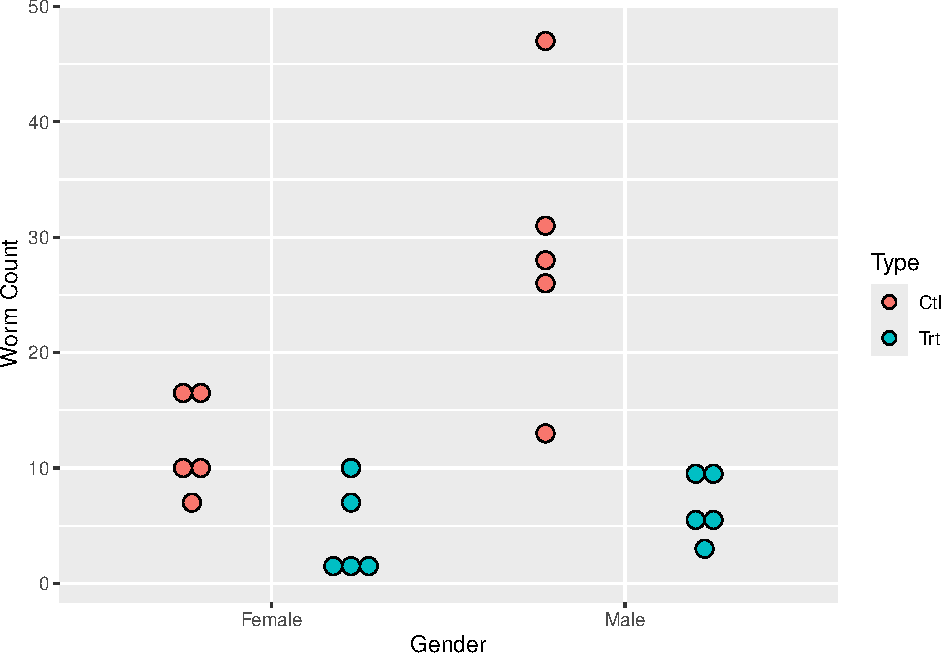
\includegraphics{index_files/figure-latex/graph1-1.pdf}
\caption{\label{fig:graph1}Individual value plot of the worm count data}
\end{figure}

\newpage

\begin{quote}
\textbf{NOTE}
There is a difference between individual value plots and dotplots. In dotplots (such as Figures 1.3 and
1.4 shown later in this chapter), each observation is represented by a dot along a number line (x-axis).
When values are close or the same, the dots are stacked. Dotplots can be used in place of histograms
when the sample size is small. Individual value plots, as shown in Figure 1.1, are used to simultaneously
display each observation for multiple groups. They can be used instead of boxplots to identify outliers and distribution shape, especially when there are relatively few observations.
\end{quote}

\hypertarget{activity-describing-the-data}{%
\section*{\texorpdfstring{Activity: \emph{Describing the Data}}{Activity: Describing the Data}}\label{activity-describing-the-data}}
\addcontentsline{toc}{section}{Activity: \emph{Describing the Data}}

\begin{quote}
\begin{enumerate}
\def\labelenumi{\arabic{enumi}.}
\tightlist
\item
  Use Figure 1.1 to visually compare the number of worms for the treatment and control groups for both
  the male and the female mice. Does each of the four groups appear to have a similar center and a similar
  spread? Are there any outliers (extreme observations that don't seem to fit with the rest of the data)?
\item
  Calculate appropriate summary statistics (e.g., the median, mean, standard deviation, and range) for
  each of the four groups. For the female mice, calculate the difference between the treatment and control
  group means. Do the same for the male mice.
\end{enumerate}
\end{quote}

The descriptive analysis in Questions 1 and 2 points to a positive treatment effect: K11777 appears to have

reduced the number of parasitic worms in this sample. But descriptive analysis is usually only the first step
in ascertaining whether an effect is real; we often conduct a significance test or create a confidence interval
to determine if chance alone could explain the effect.

Most introductory statistics courses focus on hypothesis tests that involve using a normal, t-, chi-square or F-distribution to calculate the p-value. These tests are often based on the central limit theorem. In the

schistosomiasis study, there are only five observations in each group. This is a much smaller sample size
than is recommended for the central limit theorem, especially given that Figure 1.1 indicates that the data
may not be normally distributed. Since we cannot be confident that the sample averages are normally distributed,
we will use a distribution-free test, also called a nonparametric test. Such tests do not require
the distribution of our sample statistic to have any specific form and are often useful in studies with very
small sample sizes.

\large

\textbf{MATHEMATICAL NOTE:}
For any population with mean m and finite standard deviation s, the central limit theorem states that
the sample mean x from an independent and identically distributed sample tends to follow the normal
distribution if the sample size is large enough. The mean of x is the same as the population mean, m, while
the standard deviation of x is s/1n, where n is the sample size.

\normalsize

We will use a form of nonparametric statistical inference known as a randomization hypothesis test to analyze the data from the schistosomiasis study. \textbf{Randomization hypothesis} tests are significance tests that simulate the random allocation of units to treatments many times in order to determine the likelihood of observing an outcome at least as extreme as the one found in the actual study.

\Large

\textbf{\textcolor{red}{Key Concept:}}
\textcolor{red}{\textbf{Parametric tests} (such as $z$-tests, $t$-tests, or $F$-tests) assume that data come from a population that follows a probability distribution or use the central limit theorem to make inferences about a population. \textbf{Nonparametric tests} (such as randomization tests) do not require assumptions about the distribution of the population or large sample sizes in order to make inferences about a population.}

\normalsize

We will introduce the basic concepts of randomization tests in a setting where units (mice in this example) are randomly allocated to a treatment or control group. Using a significance test, we will decide if an observed treatment effect (the observed difference between the mean responses in the treatment and control) is ``real'' or if ``random chance alone'' could plausibly explain the observed effect. The null hypothesis states that ``random chance alone'' is the reason for the observed effect. In this initial discussion, the alternative hypothesis will be onesided because we want to show that the true treatment mean (\(\mu\)treatment) is less than the true control mean (\(\mu\)control). Later, we will expand the discussion to consider modifications needed to deal with two-sided alternatives.

\hypertarget{statistical-inference-through-a-randomization-test}{%
\section{\texorpdfstring{\textbf{Statistical Inference Through a Randomization Test}}{Statistical Inference Through a Randomization Test}}\label{statistical-inference-through-a-randomization-test}}

Whether they take the form of significance tests or confidence intervals, inferential procedures rest on the fundamental question for inference: ``What would happen if we did this many times?'' Let's unpack this
question in the context of the female mice in the schistosomiasis study. We observed a difference in means
of 7.6 = 12.00 - 4.40 worms between control and treatment groups. While we expect that this large difference
reflects the effectiveness of the drug, it is possible that chance alone could explain this difference. This
``chance alone'' position is usually called the null hypothesis and includes the following assumptions:

\begin{itemize}
\tightlist
\item
  The number of parasitic worms found in the liver naturally varies from mouse to mouse.
\item
  Whether or not the drug is effective, there clearly is variability in the responses of mice to the infestation
  of schistosomes.
\item
  Each group exhibits this variability, and even if the drug is not effective, some mice do better than
  others.
\item
  The only explanation for the observed difference of 7.6 worms in the means is that the random
  allocation randomly placed mice with larger numbers of worms in the control group and mice with
  smaller numbers of worms in the treatment group.
\end{itemize}

In this study, the null hypothesis is that the treatment has no effect on the average worm count, and it

is denoted as
\textbar{} \(H_0\): \(\mu\)control = \(\mu\)treatment
Another way to write this null hypothesis is
\(H_0\): the treatment has no effect on average worm count

The research hypothesis (the treatment causes a reduction in the average worm count) is called the alternative
hypothesis and is denoted \(H_a\) (or \(H_1\)). For example,
\(H_a\): mcontrol 7 mtreatment
Another way to write this alternative hypothesis is
Ha: the treatment reduces the average worm count
Alternative hypotheses can be ``one-sided, greater than'' (as in this investigation), ``one-sided, less-than''
(the treatment causes an increase in worm count), or ``two-sided'' (the treatment mean is different, in one
direction or the other, from the control mean). We chose to test a one-sided hypothesis because there is a
clear research interest in one direction. In other words, we will take action (start using the drug) only if we
can show that K11777 reduces the worm count.

\Large

\textbf{\textcolor{red}{Key Concept:}}
\textcolor{red}{\textbf{The fundamental question for inference}: Every statistical inference procedure (parametric or nonparametric) is based on the question “How does what we observed in our data compare to what
would happen if the null hypothesis were actually true and we repeated the process many times?”
For a randomization test comparing responses for two groups, this question becomes “How does
the observed difference between groups compare to what would happen if the treatments actually
had no effect on the individual responses and we repeated the random allocation of individuals to
groups many times?”}

\normalsize

\hypertarget{activity-conducting-a-randomization-test-by-hand}{%
\section*{\texorpdfstring{Activity: \emph{Conducting a Randomization Test by Hand}}{Activity: Conducting a Randomization Test by Hand}}\label{activity-conducting-a-randomization-test-by-hand}}
\addcontentsline{toc}{section}{Activity: \emph{Conducting a Randomization Test by Hand}}

\begin{enumerate}
\def\labelenumi{\arabic{enumi}.}
\setcounter{enumi}{2}
\tightlist
\item
  To get a feel for the concept of a p-value, write each of the female worm counts on an index card.
  Shuffle the 10 index cards, and then draw five cards at random (without replacement). Call these five
  cards the treatment group and the five remaining cards the control group. Under the null hypothesis
  (i.e.~the treatment has no effect on worm counts), this allocation mimics precisely what actually happened
  in our experiment, since the only cause of group differences is the random allocation.
  \textbar{} Calculate the mean of the five cards representing the treatment group and the mean of the five
  cards representing the control group. Then find the difference between the control and treatment group means that you obtained in your allocation. To be consistent, take the control group mean minus the
  treatment group mean. Your work should look similar to the following simulation:
\end{enumerate}

{[}{[}{[}Fig\_CT{]}{]}{]}

\begin{enumerate}
\def\labelenumi{\arabic{enumi}.}
\setcounter{enumi}{3}
\item
  If you were to do another random allocation, would you get the same difference in means? Explain.
\item
  Now, perform nine more random allocations, each time computing and writing down the difference in
  mean worm count between the control group and the treatment group. Make a dotplot of the 10 differences.
  What proportion of these differences are 7.6 or larger?
\item
  If you performed the simulation many times, would you expect a large percentage of the simulations to
  result in a mean difference greater than 7.6? Explain.
\end{enumerate}

The reasoning in the previous activity leads us to the randomization test and an interpretation of the

fundamental question for inference. The fundamental question for this context is as follows: ``If the null
hypothesis were actually true and we randomly allocated our 10 mice to treatment and control groups many
times, what proportion of the time would the observed difference in means be as big as or bigger than 7.6?''
This long-run proportion is a probability that statisticians call the \textbf{p-value} of the randomization test. The
p-values for most randomization tests are found through simulations. Despite the fact that simulations do
not give exact p-values, they are usually preferred over the tedious and time-consuming process of listing
all possible outcomes. Researchers usually pick a round number such as 10,000 repetitions of the simulation
and approximate the p-value accordingly. Since this p-value is an approximation, it is often referred to as
the \textbf{empirical p-value}.

\Large

\textbf{\textcolor{red}{Key Concept:}}
\textcolor{red}{Assuming that nothing except the random allocation process is creating group differences, the p-value
of a randomization test is the probability of obtaining a group difference as large as or larger than
the group difference actually observed in the experiment.}

\Large

\textbf{\textcolor{red}{Key Concept:}}

\textcolor{red}{The calculation of an empirical p-value requires these steps:
\begin{itemize}
\item Repeat the random allocation process a number of times (N times).
\item Record, each time, whether or not the group difference exceeds or is the same as the one
observed in the actual experiment (let X be the number of times the group difference exceeds
or is the same as the one observed).
\item Compute X/N to get the p-value, the proportion of times the difference exceeds or is the same
as the observed difference.
\end{itemize}}

\large

\textbf{NOTE:}
Many researchers include the observed value as one of the possible outcomes. In this case, N = 9999
iterations are typically used and the p-value is calculated as (X + 1)/(9999 + 1). The results are very
similar whether X/10,000 or (X + 1)/(9999 + 1) is used. Including the observed value as one of the
possible allocations is a more conservative approach and protects against getting a p-value of 0. Our
observation from the actual experiment provides evidence that the true p-value is greater than zero.

\hypertarget{performing-a-randomization-test-using-a-computer-simulation}{%
\section{\texorpdfstring{\textbf{Performing a Randomization Test Using a Computer Simulation}}{Performing a Randomization Test Using a Computer Simulation}}\label{performing-a-randomization-test-using-a-computer-simulation}}

\normalsize

While physical simulations (such as the index cards activity) help us understand the process of computing an
empirical p-value, using computer software is a much more efficient way of producing an empirical p-value
based on a large number of iterations. If you are simulating 10 random allocations, it is just as easy to use index cards as a computer. However, the advantage of a computer simulation is that 10,000 random allocations
can be conducted in almost the same amount of time it takes to simulate 10 allocations. In the following
steps, you will develop a program to calculate an empirical p-value.

\hypertarget{activity-using-computer-simulations-to-conduct-a-hypothesis-test}{%
\section*{\texorpdfstring{Activity: \emph{Using Computer Simulations to Conduct a Hypothesis Test}}{Activity: Using Computer Simulations to Conduct a Hypothesis Test}}\label{activity-using-computer-simulations-to-conduct-a-hypothesis-test}}
\addcontentsline{toc}{section}{Activity: \emph{Using Computer Simulations to Conduct a Hypothesis Test}}

\begin{enumerate}
\def\labelenumi{\arabic{enumi}.}
\setcounter{enumi}{6}
\item
  Use the technology instructions provided on the CD to insert the schistosomiasis data into a statistical
  software package and randomly allocate each of the 10 female worm counts to either the treatment or the
  control group.
\item
  Take the control group average minus the K11777 treatment group average.
\item
  Use the instructions to write a program, function, or macro to repeat the process 10,000 times. Count
  the number of simulations where the difference between the group averages (control minus K11777) is
  greater than or equal to 7.6, divide that count by 10,000, and report the resulting empirical p-value.
\item
  Create a histogram of the 10,000 simulated differences between group means and comment on the
  shape of the histogram. This histogram, created from simulations of a randomization test, is called an
  empirical randomization distribution. This distribution describes the frequency of each observed
  difference (between the control and treatment means) when the null hypothesis is true.
\item
  Based on your results in Questions 9 and 10 and assuming the null hypothesis is true, about how frequently
  do you think you would obtain a mean difference as large as or larger than 7.6 by random allocation alone?
\item
  Does your answer to Question 11 lead you to believe the ``chance alone'' position (i.e., the null hypothesis
  that the mean worm count is the same for both the treatment and the control), or does it lead you to
  believe that K11777 has a positive inhibitory effect on the schistosome worm in female mice? Explain.
\end{enumerate}

Figure 1.2 shows a histogram resulting from the previous activity. A computer simulation of Question 9

resulted in a p-value of 281/10,000 = 0.0281. This result shows that random allocation alone would produce
a mean group difference as large as or larger than 7.6 only about 3\% of the time, suggesting that something
other than chance is needed to explain the difference in group means. Since the only other distinction between
the groups is the presence or absence of treatment, we can conclude that the treatment causes a reduction in
worm counts.

We conducted four more simulations, each with 10,000 iterations, which resulted in p-values of 0.0272,

0.0282, 0.0268, and 0.0285. When the number of iterations is large, the empirical randomization distribution
(such as the histogram created in Question 10) provides a precise estimate of the likelihood of all possible values of the difference between the control and treatment means. Thus, when the number of iterations is large,
well-designed simulation studies result in empirical p-values that are fairly accurate. The larger the number
of iterations (i.e., randomizations) within a simulation study, the more precise the p-value is.

\begin{figure}
\centering
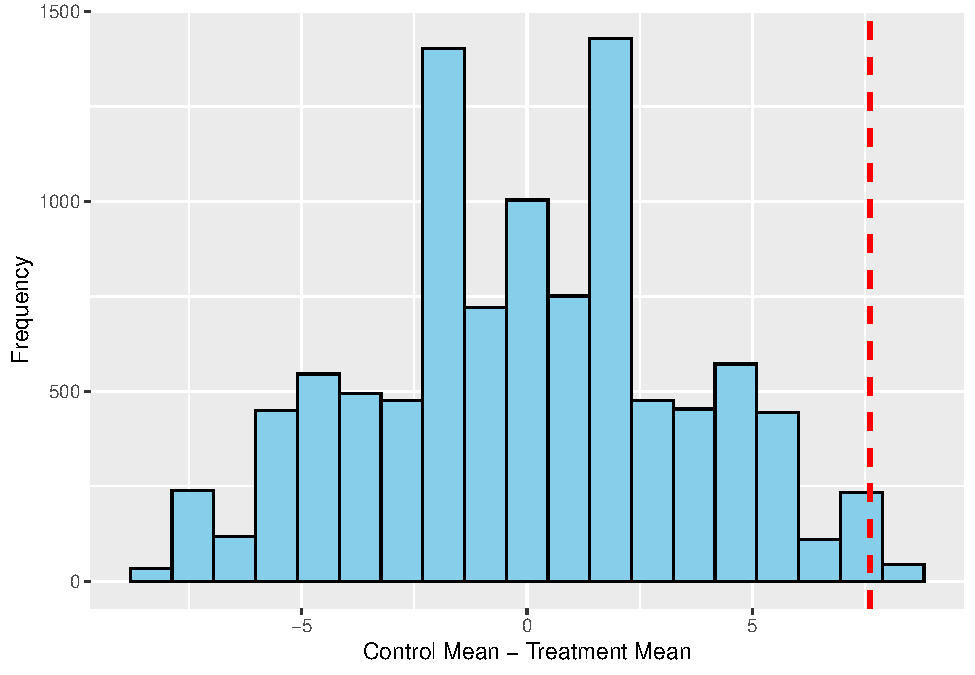
\includegraphics{index_files/figure-latex/graph2-1.pdf}
\caption{\label{fig:graph2}Histogram showing the results of a schistosomiasis simulation study. In this simulation, 281 out of 10,000 resulted in a difference greater than or equal to 7.6.}
\end{figure}

~Because the sample sizes in the schistosomiasis study are small, it is possible to apply mathematical

methods to obtain an \textbf{exact p-value} for this randomization test. An exact p-value can be calculated by writing
down the set of all possibilities (assuming each possible outcome is equally likely under the null hypothesis)
and then calculating the proportion of the set for which the difference is at least as large as the observed difference.
In the schistosomiasis study, this requires listing every possible combination in which five of the 10
female mice can be allocated to the treatment (and the other five assigned to the control). There are 252 possible
combinations. For each of these combinations, the difference between the treatment and control means
is then calculated. The exact p-value is the proportion of times in which the difference in the means is at least
as large as the observed difference of 7.6 worms. Of these 252 combinations, six have a mean difference of
7.6 and one has a mean difference greater than 7.6 (namely 8.8). Since all 252 of these random allocations are
equally likely, the exact p-value in this example is 7/252 = 0.0278. However, most real studies are too large
to list all possible samples. Randomization tests are almost always adequate, providing approximate p-values
that are close enough to the true p-value.

\large

\textbf{CAUTION:}
Conducting a two-sample t-test on the female mice provides a p-value of 0.011. This p-value of 0.011 is
accurate only if the observed test statistic (i.e., the difference between means) follows appropriate assumptions
about the distribution. Figure 1.2 demonstrates that the distributional assumptions are violated. While
the randomization test provides an approximate p-value ``close to 0.0278,'' it provides a much better estimate
of the exact p-value than does the two-sample t-test. Note that each of the five simulations listed gave a
p-value closer to the exact p-value than the one given by the two-sample t-test. \textit{Be careful not to trust a
p-value provided by statistical software unless you are certain the appropriate assumptions are met.}

\Large

\textbf{\textcolor{red}{Key Concept:}}
\textcolor{red}{The larger the number of randomizations within a simulation study, the more precise the p-value is.
When sample sizes are small or sample data clearly are not normal, a p-value derived from a randomization
test with 10,000 randomizations is typically more accurate than a p-value calculated from
a parametric test (such as the t -test).}

\normalsize

Sometimes we have some threshold p-value at or below which we will reject the null hypothesis and

conclude in favor of the alternative. This threshold value is called a significance level and is usually denoted
by the Greek letter alpha (\(\alpha\)). Common values are \(\alpha\) = 0.05 and \(\alpha\) = 0.01, but the value will depend heavily
on context and on the researcher's assessment of the acceptable risk of stating an incorrect conclusion. When
the study's p-value is less than or equal to this significance level, we state that the results are statistically
significant at level A. If you see the phrase ``statistically significant'' without a specification of \(\alpha\) the writer
is most likely assuming \(\alpha\) = 0.05, for reasons of history and convention alone. However, it is best to show
the p-value instead of simply stating a result is significant at a particular \(\alpha\)-level.

\hypertarget{two-sided-tests}{%
\section{\texorpdfstring{\textbf{Two-Sided Tests}}{Two-Sided Tests}}\label{two-sided-tests}}

The direction of the alternative hypothesis is derived from the research hypothesis. In this K11777 study, we
enter the study expecting a reduction in worm counts and hoping the data will bear out this expectation. It is
our expectation, hope, or interest that drives the alternative hypothesis and the randomization calculation. Occasionally,
we enter a study without a firm direction in mind for the alternative, in which case we use a two-sided
alternative. Furthermore, even if we hope that the new treatment will be better than the old treatment or better
than a control, we might be wrong---it may be that the new treatment is actually worse than the old treatment
or even harmful (worse than the control). Some statisticians argue that a conservative objective approach is to
always consider the two-sided alternative. For a \textbf{two-sided test}, the p-value must take into account extreme
values of the test statistic in either direction (no matter which direction we actually observe in our sample data)

\Large

\textbf{\textcolor{red}{Key Concept:}}
\textcolor{red}{The direction of the alternative hypothesis does not depend on the sample data, but instead is determined
by the research hypothesis before the data are collected.}

\normalsize

We will now make our definition of the p-value more general to allow for a wider variety of significance

testing situations. The \textbf{p-value} is the probability of observing a group difference as extreme as or more extreme
than the group difference actually observed in the sample data, assuming that there is nothing creating group
differences except the random allocation process.

\hypertarget{activity-a-two-sided-hypothesis-test}{%
\section*{\texorpdfstring{Activity: \emph{A Two-Sided Hypothesis Test}}{Activity: A Two-Sided Hypothesis Test}}\label{activity-a-two-sided-hypothesis-test}}
\addcontentsline{toc}{section}{Activity: \emph{A Two-Sided Hypothesis Test}}

\begin{enumerate}
\def\labelenumi{\arabic{enumi}.}
\setcounter{enumi}{12}
\tightlist
\item
  Run the simulation study again to find the empirical p-value for a two-sided hypothesis test to determine
  if there is a difference between the treatment and control group means for female mice.
\item
  Is the number of simulations resulting in a difference greater than or equal to 7.6 identical to the number
  of simulations resulting in a difference less than or equal to -7.6? Explain why these two values
  are likely to be close but not identical.
\item
  Explain why you expect the p-value for the two-sided alternative to be about double that for the onesided
  alternative. Hint: You may want to look at Figure 1.2
\item
  Using the two-sided alternative hypothesis, the two-sample t-test provides a p-value of 0.022.\footnote{When we do not assume equal variances Minitab uses 7 degrees of freedom providing a p-value of 0.022 while R uses
    7.929 degrees of freedom resulting in a p-value of 0.0194.} This
  p-value would provide strong evidence for rejecting the assumption that there is no difference between
  the treatment and the control (null hypothesis). However, this p-value should not be used to draw
  conclusions about this study. Explain why.
\end{enumerate}

For the above study, a simulation involving 100,000 iterations provided an empirical p-value of 0.0554.

Again, because this particular data set is small, all 252 possible random allocations can be listed to find that
the exact two-sided p-value is 14/252 = 0.0556.

\hypertarget{what-can-we-conclude-from-the-schistosomiasis-study}{%
\section{\texorpdfstring{\textbf{What Can We Conclude from the Schistosomiasis Study?}}{What Can We Conclude from the Schistosomiasis Study?}}\label{what-can-we-conclude-from-the-schistosomiasis-study}}

The key question in this study is whether K11777 will reduce the spread of a common and potentially deadly
disease. The result that you calculated from the one-sided randomization hypothesis test should have been
close to the exact p-value of 0.0278. This small p-value allows you to reject the null hypothesis and conclude
that the worm counts are lower in the female treatment group than in the female control group. In every study,
it is important to consider how random allocation and random sampling impact the conclusions.

\emph{Random allocation}: The schistosomiasis study was an \textbf{experiment} because the units (female mice)

were randomly allocated to treatment or control groups. To the best of our knowledge this experiment
controlled for any outside influences and allows us to state that there is a cause and effect relationship
between the treatment and response. Therefore, we can conclude that K11777 did cause a reduction in
the average number of schistosome parasites in these female mice.

\emph{Random sampling}: Mice for this type of study are typically ordered from a facility that breeds and raises lab

mice. It is possible that the mice in this study were biologically related or were exposed to something that
caused their response to be different from that of other mice. Similarly, there are risks in simply assuming
that male mice have the same response as females, so the end-of-chapter exercises provide an opportunity to conduct a separate test on the male mice. Since our sample of 10 female mice was not selected at random
from the population of all mice, we should question whether the results from this study hold for all mice.

More importantly, the results have not shown that this new drug will have the same impact on humans
as it does on mice. In addition, even though we found that K11777 does cause a reduction in worm counts,
we did not specifically show that it will reduce the spread of the disease. Is the disease less deadly if only two
worms are in the body instead of 10? Statistical consultants aren't typically expected to know the answers to
these theoretical, biological, or medical types of questions, but they should ask questions to ensure that the
study conclusions match the hypothesis that was tested. In most cases, drug tests require multiple levels of
studies to ensure that the drug is safe and to show that the results are consistent across the entire population of
interest. While this study is very promising, much more work is needed before we can conclude that K11777
can reduce the spread of schistosomiasis in humans.

\hypertarget{a-closer-look-nonparametric-methods}{%
\section*{\texorpdfstring{\emph{A Closer Look: Nonparametric Methods}}{A Closer Look: Nonparametric Methods}}\label{a-closer-look-nonparametric-methods}}
\addcontentsline{toc}{section}{\emph{A Closer Look: Nonparametric Methods}}

\hypertarget{permutation-tests-versus-randomization-tests}{%
\section{\texorpdfstring{\textbf{Permutation Tests versus Randomization Tests}}{Permutation Tests versus Randomization Tests}}\label{permutation-tests-versus-randomization-tests}}

The random allocation of experimental units (e.g., mice) to groups provides the basis for statistical inference in
a randomized comparative experiment. In the schistosomiasis K11777 treatment study, we used a significance
test to ascertain whether cause and effect was at work. In the context of the random allocation study design,
we called our significance test a randomization test.
\textbar{} In \textbf{observational studies}, subjects are not randomly allocated to groups. In this context, we apply the
same inferential procedures as in the previous experiment, but we commonly call the significance test a
\textbf{permutation test} rather than a randomization test.\footnote{This text defines a randomization test as a permutation test that is based on random allocation. Some statisticians do not
  distinguish between permutation tests and randomization tests. They call simulation studies permutation tests, whether
  they are based on observational studies or experiments.} More importantly, in observational studies, the results
of the test cannot typically be used to claim cause and effect; a researcher should exhibit more caution in the
interpretation of results.

\large

\textbf{NOTE:}
\textcolor{black}{The permutation test does not require that the data (or the sampling distribution) follow a normal distribution.
However, the null hypothesis in a permutation test assumes that samples are taken from two populations
that are similar. So, for example, if the two population variances are very different, the p-value of a
permutation test may not be reliable. However, the two-sample t-test (taught in most introductory courses)
allows us to assume unequal variances.}

\Large

\textbf{\textcolor{red}{Key Concept:}}
\textcolor{red}{Whereas in experiments units are randomly allocated to treatment groups, observational studies do not
impose a treatment on a unit. Because the random allocation process protects against potential biases
caused by extraneous variables, experiments are often used to show causation.}

\hypertarget{age-discrimination-study}{%
\section*{Age Discrimination Study}\label{age-discrimination-study}}
\addcontentsline{toc}{section}{Age Discrimination Study}

\normalsize

Westvaco is a company that produces paper products. In 1991, Robert Martin was working in the engineering
department of the company's envelope division when he was laid off in Round 2 of several rounds of layoffs
by the company.3 He sued the company, claiming to be the victim of age discrimination. The ages of the 10
workers involved in Round 2 were: 25, 33, 35, 38, 48, 55, 55, 55, 56, and 64. The ages of the three people
laid off were 55, 55, and 64.

Figure 1.3 shows a comparative dotplot for age by layoff category. This dotplot gives the impression that

Robert Martin may have a case: It appears as if older workers were more likely to be laid off. But we know
enough about variability to be cautious.

\begin{figure}
\centering
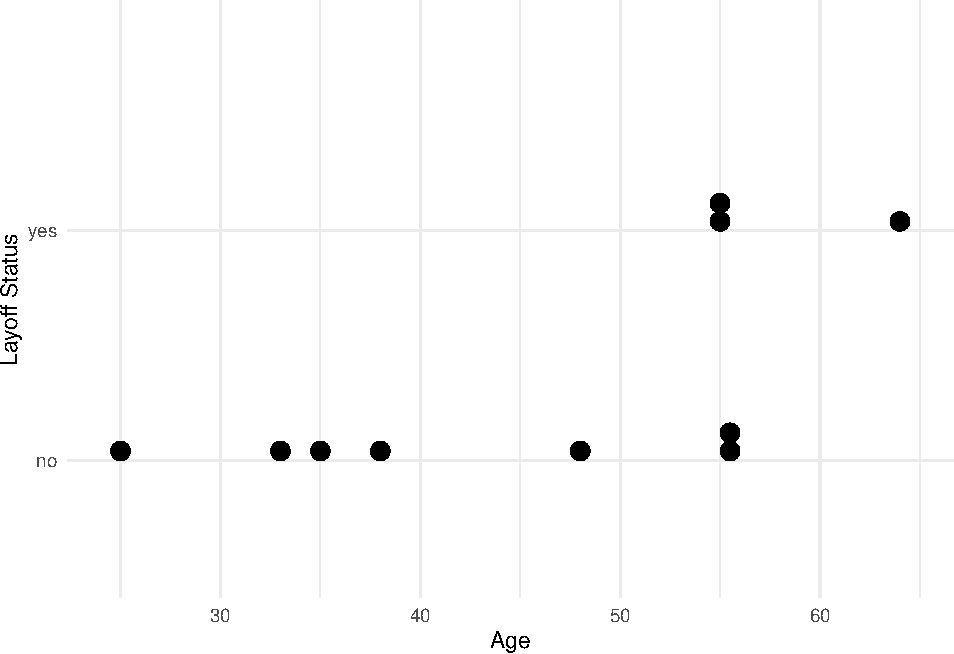
\includegraphics{index_files/figure-latex/graph3-1.pdf}
\caption{\label{fig:graph3}Dotplot of age in years of worker versus layoff (whether he or she was laid off)}
\end{figure}

\hypertarget{extended-activity-is-there-evidence-of-age-discrimination}{%
\section*{\texorpdfstring{Extended Activity: \emph{Is There Evidence of Age Discrimination?}}{Extended Activity: Is There Evidence of Age Discrimination?}}\label{extended-activity-is-there-evidence-of-age-discrimination}}
\addcontentsline{toc}{section}{Extended Activity: \emph{Is There Evidence of Age Discrimination?}}

Data set: \texttt{Age}
17. Conduct a permutation test to determine whether the observed difference between means is likely to
occur just by chance. Use \texttt{Age} as the response variable and \texttt{Layoff} as the explanatory variable. Here
we are interested in only a one-sided hypothesis test to determine if the mean age of people who were
laid off is higher than the mean age of people who were not laid off.

\begin{enumerate}
\def\labelenumi{\arabic{enumi}.}
\setcounter{enumi}{17}
\tightlist
\item
  Modify the program/macro you created in Question 17 to conduct a one-sided hypothesis test to determine
  if the median age of people who were laid off is higher than the median age of people who were
  not laid off. Report the p-value and compare your results to those in Question 17.
\end{enumerate}

~Since there was no random allocation (i.e., people were not randomly assigned to a layoff group),

statistical significance does not give us the right to assert that greater age is \emph{causing} a difference in being
laid off. The null hypothesis in this context becomes ``The observed difference could be explained as if
by random allocation alone.'' That is, we proceed as any practicing social scientist must when working
with observational data. We ``imagine'' an experiment in which workers are randomly allocated to a
layoff group and then determine if the observed average difference between the ages of laid-off workers
and those not laid off is significantly larger than would be expected to occur by chance in a randomized
comparative experiment.
\textbar{} While age could be the cause for the difference---hence proving an allegation of age discrimination---
there are many other possibilities (i.e., extraneous variables), such as the educational levels of the
workers, their competence to do the job, and ratings on past performance evaluations. Rejecting the
``as if by random allocation'' hypothesis in the nonrandomized context can be a useful step toward
establishing causality; however, it cannot establish causality unless the extraneous variables have been
properly accounted for.
\textbar{} In the actual court case, data from all three rounds of layoffs were statistically analyzed. The analysis
showed some evidence that older people were more likely to be laid off; however, Robert Martin ended up
settling out of court.

\hypertarget{permutation-and-randomization-tests-for-matched-pairs-designs}{%
\section{\texorpdfstring{\textbf{Permutation and Randomization Tests for Matched Pairs Designs}}{Permutation and Randomization Tests for Matched Pairs Designs}}\label{permutation-and-randomization-tests-for-matched-pairs-designs}}

The ideas developed in this chapter can be extended to other study designs, such as a basic two-variable design
called a matched pairs design. In a matched pairs design, each experimental unit provides both measurements
in a study with two treatments (one of which could be a control). Conversely, in the completely randomized
situation of the schistosomiasis K11777 treatment study, half the units were assigned to control and half to
treatment; no mouse received both treatments.

\hypertarget{music-and-relaxation}{%
\section*{Music and Relaxation}\label{music-and-relaxation}}
\addcontentsline{toc}{section}{Music and Relaxation}

Grinnell College students Anne Tillema and Anna Tekippe conducted an experiment to study the effect of
music on a person's level of relaxation. They hypothesized that fast songs would increase pulse rate more
than slow songs. The file called Music contains the data from their experiment. They decided to use a person's
pulse rate as an operational definition of the person's level of relaxation and to compare pulse rates for two selections of music: a fast song and a slow song. For the fast song they chose ``Beyond'' by Nine Inch
Nails, and for the slow song they chose Rachmaninoff's ``Vocalise.'' They recruited 28 student subjects for
the experiment.

Anne and Anna came up with the following experimental design. Their fundamental question

involved two treatments: (1) listening to the fast song and (2) listening to the slow song. They could
have randomly allocated 14 subjects to hear the fast song and 14 subjects to hear the slow song, but
their more efficient approach was to have each subject provide both measurements. That is, each subject
listened to both songs, giving rise to two data values for each subject, called a matched pairs. Randomization
came into play when it was decided by a coin flip whether each subject would listen first to the
fast song or the slow song.

\large

\textbf{NOTE:}
\textcolor{black}{There are several uses of randomness mentioned in this chapter. The emphasis of this chapter is on the
use of \textbf{randomization tests} for statistical inference. Most introductory statistics courses discuss random
\textbf{sampling} from a population, which allows the results of a specific study to be generalized to a larger
population. In experiments, units are \textbf{randomly allocated to groups} which allows researchers to make
statements about causation. In this example, Anne and Anna \textbf{randomize the order} to prescribe two
conditions on a single subject.}

\normalsize

~Specifically, as determined by coin flips, half the subjects experienced the following procedure:

{[}one minute of rest; measure pulse (prepulse){]} \(>\) {[}listen to fast song for 2 minutes; measure pulse
for second minute (fast song pulse){]} \(>\) {[}rest for one minute{]} \(>\) {[}listen to slow song for 2 minutes;
measure pulse for second minute (slow song pulse){]}.

The other half experienced the procedure the same way except that they heard the slow song first and

the fast song second.
\textbar{} Each subject gives us two measurements of interest for analysis: (1) fast song pulse minus prepulse
and (2) slow song pulse minus prepulse. In the data file, these two measurements are called \texttt{Fastdiff} and
\texttt{Slowdiff}, respectively.

Figure 1.4 shows a dotplot of the 28 \texttt{Fastdiff}-minus-\texttt{Slowdiff} values. Notice that positive numbers

predominate and the mean difference is 1.857 beats per minute, both suggesting that the fast song does indeed
heighten response (pulse rate) more than the slow song. We need to confirm this suspicion with a randomization
test.

To perform a randomization test, we mimic the randomization procedure of the study design. Here,

the randomization determined the order in which the subject heard the songs, so randomization is applied
to the two measurements of interest for each subject. To compute a p-value, we determine how frequently
we would obtain an observed difference as large as or larger than 1.857.

\begin{verbatim}
#> Bin width defaults to 1/30 of the range of the data. Pick
#> better value with `binwidth`.
\end{verbatim}

\begin{figure}
\centering
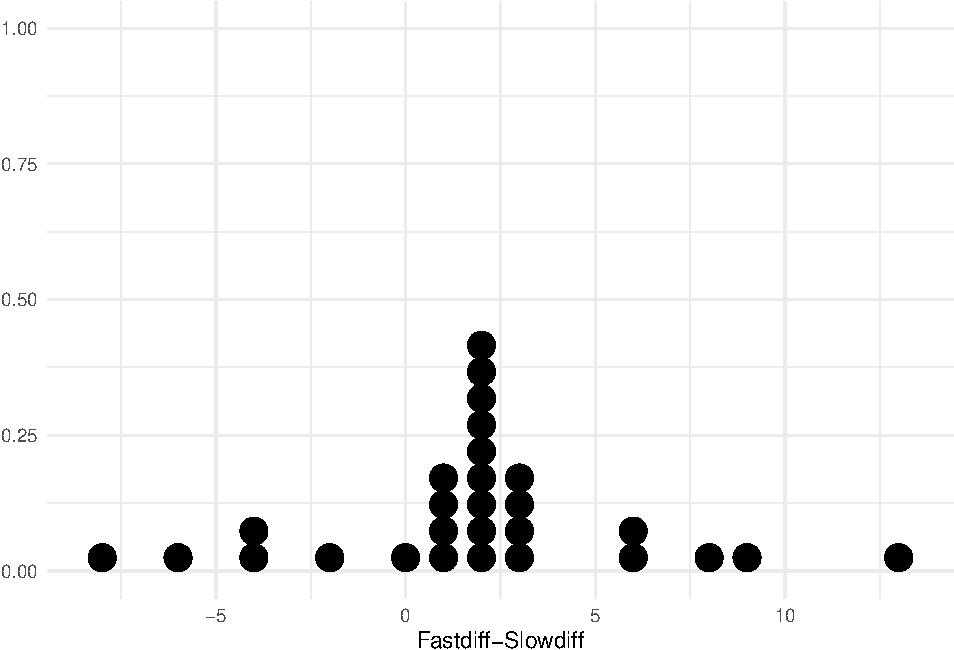
\includegraphics{index_files/figure-latex/graph4-1.pdf}
\caption{\label{fig:graph4}Dotplot of the difference in pulse rates for each of the 28 subjects.}
\end{figure}

\hypertarget{extended-activity-testing-the-effect-of-music-on-relaxation}{%
\section*{\texorpdfstring{Extended Activity: \emph{Testing the Effect of Music on Relaxation}}{Extended Activity: Testing the Effect of Music on Relaxation}}\label{extended-activity-testing-the-effect-of-music-on-relaxation}}
\addcontentsline{toc}{section}{Extended Activity: \emph{Testing the Effect of Music on Relaxation}}

Data set: \texttt{Music}

\begin{enumerate}
  \setcounter{enumi}{18}  

  \item Before they looked at the data, Anne and Anna decided to use a one-sided test to see whether fast
  music increased pulse rate more than slow music. Why is it important to determine the direction of the
  test before looking at the data?

  \item Create a simulation to test the Music data. Use the technology instructions provided to randomly
  multiply a 1 or a -1 by each observed difference. This randomly assigns an order (`Fastdiff -
  Slowdiff` or `Slowdiff - Fastdiff`). Then, for each iteration, calculate the mean difference. The
  p-value is the proportion of times your simulation found a mean difference greater than or equal to
  1.857.
  \begin{enumerate}
    \item Create a histogram of the mean differences. Mark the area on the histogram that represents your p-value.

    \item Use the p-value to state your conclusions in the context of the problem. Address random allocation
    and random sampling (or lack of either) when stating your conclusions.
  \end{enumerate}
\end{enumerate}

\large

\textbf{CAUTION:}
\textcolor{black}{The type of randomization in Question 20 does not account for extraneous variables such as a great love
for Nine Inch Nails on the part of some students or complete boredom with this band on the part of others
(i.e., “musical taste” is a possible confounder that randomizing the order of listening cannot randomize
away). There will always be a caveat in this type of study, since we are rather crudely letting one Nine
Inch Nails song “represent” fast songs.}

\hypertarget{the-bootstrap-distribution}{%
\section{\texorpdfstring{\textbf{The Bootstrap Distribution}}{The Bootstrap Distribution}}\label{the-bootstrap-distribution}}

\normalsize

Bootstrapping is another simulation technique that is commonly used to develop confidence intervals and
hypothesis tests. Bootstrap techniques are useful because they generalize to situations where traditional methods
based on the normal distribution cannot be applied. For example, they can be used to create confidence intervals
and hypothesis tests for any parameter of interest, such as a median, ratio, or standard deviation. Bootstrap
methods differ from previously discussed techniques in that they sample \textbf{with replacement} (randomly draw
an observation from the original sample and put the observation back before drawing the next observation).
\textbar{} Permutation tests, randomization tests, and bootstrapping are often called \textbf{resampling techniques}
because, instead of collecting many different samples from a population, we take repeated samples (called
resamples) from just one random sample.

\hypertarget{extended-activity-creating-a-sampling-distribution-and-a-bootstrap-distribution}{%
\section*{\texorpdfstring{Extended Activity: \emph{Creating a Sampling Distribution and a Bootstrap Distribution}}{Extended Activity: Creating a Sampling Distribution and a Bootstrap Distribution}}\label{extended-activity-creating-a-sampling-distribution-and-a-bootstrap-distribution}}
\addcontentsline{toc}{section}{Extended Activity: \emph{Creating a Sampling Distribution and a Bootstrap Distribution}}

Data set: \texttt{ChiSq}

\begin{enumerate}
  \setcounter{enumi}{20} 
\item The file ChiSq contains data from a highly skewed population (with mean 0.9744 and standard
deviation 1.3153).
a. Take 1000 simple random samples of size 40 and calculate each mean (x). Plot the histogram of the
1000 sample means. The distribution of sample means is called the sampling distribution.
b. What does the central limit theorem tell us about the shape, center, and spread of the sampling distribution
in this example?
c. Calculate the mean and standard deviation of the sampling distribution in Part A. Does the sampling
distribution match what you would expect from the central limit theorem? Explain.
\item Take one simple random sample of size 40 from the ChiSq data.
a. Take 1000 resamples (1000 samples of 40 observations with replacement from the one simple
random sample).
b. Calculate the mean of each resample (x*) and plot the histogram of the 1000 resample means. This
distribution of resample means is called the bootstrap distribution.
c. Compare the shape, center, and spread of the simulated histograms from Part B and Question
21 Part A. Are they similar?
\item Instead of using the sample mean, create a sampling distribution and bootstrap distribution of the standard
deviation of the ChiSq data using a sample size of 40. Compare the shape, center, and spread of
the simulated histograms and compare the mean and standard deviation of the distributions.
\end{enumerate}

\Large

\textbf{\textcolor{red}{Key Concept:}}
\textcolor{red}{The bootstrap method takes one simple random sample of size n from a population. Then many resamples
(with replacement) are taken from the original simple random sample. Each resample is the same
size as the original random sample. The statistic of interest is calculated from each resample and used
to create a bootstrap distribution.}

\normalsize

In many real-world situations, the process used in Question 21 is not practical because collecting more

than one simple random sample is too expensive or time consuming. While the approach in Question 22 is
computer intensive, it is simple and convenient since it uses only one simple random sample. The key idea
behind bootstrap methods is the assumption that the original sample represents the population, so resamples
from the one simple random sample can be used to represent samples from the population, as is done in Question
22. Thus, the bootstrap distribution provides an approximation of the sampling distribution.

Most traditional methods of statistical inference involve collecting one sample and calculating the sample

mean. Then, based on the central limit theorem, assumptions are made about the shape and spread of the
sampling distribution. In Question 22 we used one sample to calculate the sample mean and then used the
bootstrap distribution to estimate the shape and spread of the sampling distribution.

The central limit theorem tells us about the shape and spread of the sample mean. A key advantage of

the bootstrap distribution is that it works for any parameter of interest. Thus, the bootstrap distribution can be
used to estimate the shape and spread for any sampling distribution of interest.

\large

\textbf{CAUTION:}
\textcolor{black}{When sample sizes are small, one simple random sample may not represent the population very well.
However, with larger sample sizes, the bootstrap distribution does represent the sampling distribution.}

\normalsize

Figure 1.5 shows the sampling distribution and the bootstrap distribution when a sample size of 10 is used to estimate the mean of the \texttt{ChiSq} data. Notice that the spreads for both histograms are

roughly equivalent. The central limit theorem tells us that the standard deviation of the sampling distribution (the distribution of \(\bar{x}\) ) should be \(\sigma\)/\(\sqrt{n}\) = 1.3153/\(\sqrt{10}\) = 0.4159. The standard deviation of the bootstrap distribution is 0.4541, which is a reasonable estimate of the standard deviation of the sampling distribution. In addition, both graphs have similar, right-skewed shapes. The strength of the bootstrap method is that it provides accurate estimates of the shape and spread of the sampling distribution. In general, histograms from the bootstrap distribution will have a similar shape and spread as histograms
from the sampling distribution.

\begin{verbatim}
#> [1] "1.465279886"
\end{verbatim}

{[}{[}{[}Fig1,5{]}{]}{]}

The bootstrap method does not improve our estimate of the population mean. The mean of the sampling distribution in Question 21 will typically be very close to the population mean. But the mean of the bootstrap distribution in Question 22 typically will not be as accurate, because it is based on only one simple random sample. Ideally, we would like to know how close the statistic from our original sample is to the population parameter. A statistic is biased if it is not centered at the value of the population parameter. We can use the bootstrap distribution to estimate the bias of a statistic. The difference between the original sample mean and the bootstrap mean is called the \textbf{bootstrap estimate of bias}.

\Large

\textbf{\textcolor{red}{Key Concept:}}
\textcolor{red}{The estimate of the mean (or any parameter of interest) provided by the bootstrap distribution is not any better than the estimate provided by the observed statistic from the original simple random sample. However, the shape and spread of the bootstrap distribution will be similar to the shape and spread of the sampling distribution. The bootstrap technique can be used to estimate sampling distribution shapes and standard deviations that cannot be calculated theoretically.}

\normalsize

\hypertarget{using-bootstrap-methods-to-create-confidence-intervals}{%
\section{\texorpdfstring{\textbf{Using Bootstrap Methods to Create Confidence Intervals}}{Using Bootstrap Methods to Create Confidence Intervals}}\label{using-bootstrap-methods-to-create-confidence-intervals}}

A \textbf{confidence interval} gives a range of plausible values for some parameter. This is a range of values surrounding an observed estimate of the parameter---an estimate based on the data. To this range of values we attach a level of confidence that the true parameter lies in the range. An alpha-level, \(\alpha\), is often used to specify the level of confidence. For example, when \(\alpha\) = 0.05, we have a 100(1 - \(\alpha\)), = 95\(\%\) confidence level. Thus, a 100(1 - \(\alpha\)), confidence interval gives an estimate of where we think the parameter is and how precisely we have it pinned down.

\hypertarget{bootstrap-t-confidence-intervals-}{%
\section{\texorpdfstring{*\textbf{Bootstrap t Confidence Intervals}\{-\}}{*Bootstrap t Confidence Intervals\{-\}}}\label{bootstrap-t-confidence-intervals-}}

If the bootstrap distribution appears to be approximately normal, it is typically safe to assume that a
t-distribution can be used to calculate a 100(1 - \(\alpha\)), confidence interval for \(\mu\), often called a bootstrap
t confidence interval:

\begin{equation} 
  \bar{x} \pm t^*\left(S^*\right)
  \tag{1.1} \label{eq:1_1}
\end{equation}

where \(S^*\) is the standard deviation of the bootstrap distribution and \(t^*\) is the critical value of the t-distribution with n - 1 degrees of freedom.

The one simple random sample of size n = 10 used to create the bootstrap distribution in Figure 1.5b has a mean of \(\bar{x}\) = 1.238 and a standard deviation of s = 1.490. The bootstrap distribution in Figure 1.5b has a mean of \(\bar{x}^*\) = 1.249 and a standard deviation of \(S^*\) = 0.4541. Notice that Formula (1.1) uses the mean from the original sample but uses the bootstrap distribution to estimate the spread. If we \emph{incorrectly assume} that the sampling distribution in Figure 1.5 is normal, a 95\% bootstrap t confidence interval for \(\mu\) is given by

\begin{equation} 
  \bar{x} \pm t^*\left(S^*\right) = 1.238 \pm 2.262(0.4541)
\end{equation}

where \(t^*\) = 2.262 is the critical value corresponding to the 97.5th percentile of the t-distribution with n - 1 = 9
degrees of freedom. Thus, the 95\% confidence interval for \(\mu\) is (0.211, 2.265).

\large

\textbf{MATHEMATICAL NOTE:}
\textcolor{black}{The bootstrap t confidence interval is similar to the traditional one-sample t confidence interval. The key difference
is that the bootstrap distribution estimates the standard error of the statistic with S* instead of s/$\sqrt{n}$.
When the data are not skewed and have no clear outliers, parametric tests are very effective with relatively
small sample sizes (10–30 observations may be enough to use the t-distribution). The following formula
uses the t-distribution to calculate a 100(1 - $\alpha$), confidence interval for the mean of a normal population:
\begin{equation} 
  \bar{x} + t^*\left(\frac{s}{\sqrt{n}}\right)
  \tag{1.2} \label{eq:1_2}
\end{equation} 
where s/$\sqrt{n}$ is the standard error of x and t* is the critical value of the t-distribution with n - 1 degrees
of freedom. Using the original sample of size 10 with mean 1.238 and standard deviation 1.490, we find
that a 95% confidence interval for $\mu$ is  (0.172, 2.304). However, this confidence interval is appropriate for
sample means only when the sampling distribution is approximately normal. If the data are skewed, even
sample sizes greater than 30 may not be large enough to make the sampling distribution appear normal.
}

\normalsize

With skewed data or small sample sizes (if the original data are not normally distributed), parametric
methods (which are based on the central limit theorem) are not appropriate. In Figure 1.5 we see that the
sampling distribution is skewed to the right. \emph{Thus, with a sample size of 10, neither the traditional onesample
t confidence interval nor the bootstrap t confidence interval is reliable in this example}. However,
with a sample size of 40, the histograms in Questions 21 and 22 should tend to look somewhat normally
distributed.

\hypertarget{bootstrap-percentile-confidence-intervals}{%
\section*{Bootstrap Percentile Confidence Intervals}\label{bootstrap-percentile-confidence-intervals}}
\addcontentsline{toc}{section}{Bootstrap Percentile Confidence Intervals}

Bootstrap percentile confidence intervals are found by calculating the appropriate percentiles of the bootstrap distribution. To find a 100(1 - \(\alpha\)) confidence interval, take the \(\alpha\)/2 * 100 percentile of each tail of the bootstrap distribution. For example, to find a 95\% confidence interval for \(\mu\), sort all the observations from the bootstrap distribution and find the values that represents the 2.5th and 97.5th percentiles of the bootstrap distribution. The
2.5th percentile of the bootstrap distribution in Figure 1.5b is 0.546, and the 97.5th percentile is 2.282. Thus,
a 95\% confidence interval for \(\mu\) is (0.546, 2.282).
Notice that the percentile confidence interval is not centered at the sample mean. Since the bootstrap
distribution is right skewed, the right side of the confidence interval (2.282 - 1.238 = 1.044) is wider than
the left side of the confidence interval (1.238 - 0.546 = 0.692). This lack of symmetry can influence the
accuracy of the confidence interval.

\Large

\textbf{\textcolor{red}{Key Concept:}}
\textcolor{red}{A bootstrap percentile confidence interval contains the middle 100(1 - a)% of the bootstrap distribution.
If the bootstrap distribution is symmetric and is centered on the observed statistic (i.e., not biased),
percentile confidence intervals work well.}

\normalsize

\hypertarget{when-to-use-bootstrap-confidence-intervals}{%
\section*{When to Use Bootstrap Confidence Intervals}\label{when-to-use-bootstrap-confidence-intervals}}
\addcontentsline{toc}{section}{When to Use Bootstrap Confidence Intervals}

Bootstrap methods are extremely useful when we cannot use theory, such as the central limit theorem, to
approximate the sampling distribution. Thus, bootstrap methods can be used to create confidence intervals
for essentially any parameter of interest, while the central limit theorem is limited to only a few parameters
(such as the population mean).\footnote{Theoretical methods allow distributional tests for more than just the population mean. However, for purposes of this text it is sufficient to understand that distributional methods tend to be more complicated and are limited to testing only a few
  parameters that could be of interest.} However, bootstrap methods are not always reliable.

Small sample sizes still produce problems for bootstrap methods. When the sample size is small, (1) the sample statistic may not accurately estimate the population parameter, (2) the distribution of sample means is less likely to be symmetric, and (3) the shape and spread of the bootstrap distribution may not accurately represent those of the true sampling distribution.

In addition, bootstrap methods do not work equally well for all parameters. For example, the end-ofchapter

exercises show that bootstrapping often provides unreliable bootstrap distributions for median values because the median of a resample is likely to have only a few possible values. Thus, confidence intervals for medians should be used only with large (n \(\geq\) 100) sample sizes.

It is not easy to determine whether bootstrap methods provide appropriate confidence intervals. The bootstrap t and bootstrap percentile confidence intervals are often compared to each other. While the percentile confidence interval tends to be more accurate, neither of the two should be used if the intervals are not relatively

close. If the bootstrap distribution is skewed or biased, other methods should be used to find confidence intervals. More advanced bootstrap methods (such as BCa and tilting confidence intervals) are available that are generally accurate when bias or skewness exists in the bootstrap distribution.\(^5\)

\hypertarget{extended-activityestimating-salaries-of-medical-faculty}{%
\section*{\texorpdfstring{Extended Activity:\emph{Estimating Salaries of Medical Faculty}}{Extended Activity:Estimating Salaries of Medical Faculty}}\label{extended-activityestimating-salaries-of-medical-faculty}}
\addcontentsline{toc}{section}{Extended Activity:\emph{Estimating Salaries of Medical Faculty}}

Data set: \texttt{MedSalaries}.
The file \texttt{MedSalaries} is a random sample of n = 100 salaries of medical doctors who were teaching at United States universities in 2009.

\begin{enumerate}
  \setcounter{enumi}{23} 
  \item Create a bootstrap distribution of the mean by taking 1000 resamples (with replacement). Create a bootstrap t confidence interval and a bootstrap percentile distribution to estimate the mean salaries.
  \item Create a bootstrap distribution of the standard deviation by taking 1000 resamples (with replacement). Create a bootstrap t confidence interval and a bootstrap percentile distribution to estimate the population standard deviation.
  \item Use Formula (1.2) to create a 95% confidence interval for the mean. Compare this confidence intervals to those in Part A. Would you expect these intervals to be similar? Why or why not?
  \item Explain why Formula (1.2) cannot be used to create a 95% confidence interval for the standard deviation.
\end{enumerate}

\hypertarget{relationship-between-the-randomization-test-and-the-two-sample-t-test}{%
\section{\texorpdfstring{\textbf{Relationship Between the Randomization Test and the Two-Sample t-Test}}{Relationship Between the Randomization Test and the Two-Sample t-Test}}\label{relationship-between-the-randomization-test-and-the-two-sample-t-test}}

R.A. Fisher, perhaps the preeminent statistician of the 20th century, introduced the randomization test in the context of a two-group randomly allocated experiment in his famous 1935 book, \emph{Design of Experiments}.\(^6\) At that time he acknowledged that the randomization test was not practical because of the computational
intensity of the calculation. Clearly, 1935 predates modern computing. Indeed, Efron and Tibshirani describe the permutation test as ``a computer-intensive statistical technique that predates computers.''\(^7\) Fisher went on to assert that the classical two-sample t-test (for independent samples) approximates the randomization test very well. Ernst cites references to several approximations to the randomization tests using classical and computationally tractable methods that have been published over time.\(^8\)

If you have seen two-sample tests previously, it is likely to have been in the context of what Ernst calls the population model, which he distinguishes from the randomization model. In a \textbf{population model}, units are selected at random from one or more populations. Most observational studies are population models. One simple case of a population model involves comparing two separate population means. In this case, we can take two independent simple random samples and use the classic two-sample t-test to make the comparison.

In a *\textbf{randomization model}, a fixed number of experimental units are randomly allocated to treatments. Most experiments are randomization models. In randomization models such as the schistosomiasis example,

the two samples are formed from a collection of available experimental units that are randomly divided into two groups. Since there are a fixed number of units, the groups are not completely independent. For example,
if one of the 10 male mice had a natural resistance to schistosomiasis and was randomly placed in the treatment group, we would expect the control group to have a slightly higher worm count. Since the two groups are not completely independent, the assumptions of the classic two-sample t-test are violated. Even if the sample sizes in the schistosomiasis study were much larger, the randomization test would be a more appropriate test than the two-sample t-test. However, empirical evidence has shown that the two-sample t-test is a very good approximation to the randomization test when sample sizes are large enough. We are fortunate that, in this age of modern computing, we no longer have to routinely compromise by using the t-test to approximate the randomization test.

\Large

\textbf{\textcolor{red}{Key Concept:}}
\textcolor{red}{Historically, the two-sample t -test was used to approximate the p-value in randomization models because randomization tests were too difficult to compute. However, now that computers can easily simulate random assignment to groups, randomization tests should be used to calculate p-values for randomization models, especially if sample sizes are fairly small.}

\normalsize

\hypertarget{wilcoxon-rank-sum-tests-for-two-independent-samples}{%
\section{\texorpdfstring{\textbf{Wilcoxon Rank Sum Tests for Two Independent Samples}}{Wilcoxon Rank Sum Tests for Two Independent Samples}}\label{wilcoxon-rank-sum-tests-for-two-independent-samples}}

The \textbf{Wilcoxon rank sum test}, also called the two-sample \textbf{Mann-Whitney test}, makes inferences about the difference between two populations based on data from two independent random samples. This test ranks observations from two samples by arranging them in order from smallest to largest.

Focusing on ranks instead of the actual observed values allows us to remove assumptions about the normal distribution. Rank-based tests have been used for many years. However, rank-based methods (discussed

in this section and the next section) are much less accurate than methods based on simulations. In general, randomization tests, permutation tests, or bootstrap methods should be used whenever possible.

The following example examines whether pitchers and first basemen who play for National League baseball teams have the same salary distribution. The null and alternative hypotheses are written as,

\(H_0\): the distribution of the salaries is the same for pitchers and first basemen
\(H_a\): the distribution of the salaries is different for pitchers and first basemen

Table 1.2 shows the salaries of five pitchers and five first basemen who were randomly selected from all National League baseball players. Table 1.3 ranks each of the players based on 2005 salaries.

Note that if two players had exactly the same salary, standard practice would be to average the ranks of the tied values.

\begin{table}

\caption{\label{tab:table2}Randomly selected pitchers and first baseman from 2005 National League baseball teams.}
\centering
\begin{tabular}[t]{lllr}
\toprule
Team & Position & Name & Salary(\textbackslash{}\$)\\
\midrule
Milwaukee Brewers & Pitcher & Obermueller, Wes & 342000\\
Houston Astros & Pitcher & Backe, Brandon & 350000\\
Atlanta Braves & Pitcher & Sosa, Jorge & 650000\\
Atlanta Braves & Pitcher & Thomson, John & 4250000\\
Cincinnati Reds & First Baseman & Casey, Sean & 7800000\\
\addlinespace
Arizona Diamondbacks & First Baseman & Green, Shawn & 7833333\\
San Diego Padres & First Baseman & Nevin, Phil & 9625000\\
New York Mets & Pitcher & Glavine, Tom & 10765608\\
Colorado Rockies & First Baseman & Helton, Todd & 12600000\\
Philadelphia Phillies & First Baseman & Thome, Jim & 13166667\\
\bottomrule
\end{tabular}
\end{table}

\begin{table}

\caption{\label{tab:table3}Ranking the 10 randomly selected 2005 National League baseball players.}
\centering
\begin{tabular}[t]{lllllllllll}
\toprule
Position & Pr & Pr & Pr & Pr & FB & FB & FB & Pr & FB & FB\\
Salary & 342 & 350 & 650 & 4250 & 7800 & 7833 & 9625 & 10766 & 12600 & 13167\\
Rank & 1 & 2 & 3 & 4 & 5 & 6 & 7 & 8 & 9 & 10\\
\bottomrule
\end{tabular}
\end{table}

For the Wilcoxon rank sum test, we define the following terms:

\begin{itemize}
\tightlist
\item
  \(n_1\) is the sample size for the first group (5 for the pitcher group in this example)
\item
  \(n_2\) is the sample size for the second group (5 for the first baseman group in this example)
\item
  N= \(n_1\) + \(n_2\)
\item
  W, the Wilcoxon rank sum statistic, is the sum of the ranks in the first group
  (1 + 2 + 3 + 4 + 8 = 18)
\end{itemize}

If the two groups are from the same continuous distribution, then W has a mean,

\begin{equation} 
  \mu_W = \frac{n_1(N+1)}{2} = \frac{5(11)}{2}=27.5
  \tag{1.3} \label{eq:1_3}
\end{equation}

and standard deviation\(^9\)

\begin{equation} 
  \sigma_W = \sqrt{\frac{n_1n_2(N+1)}{12}} = \sqrt{\frac{(5)(5)(11)}{12}}= 4.787
  \tag{1.4} \label{eq:1_4}
\end{equation}

If W is far from \(\mu_W\), then the Wilcoxon rank sum test rejects the hypothesis that the two populations have identical distributions---that is, rejects \(H_0\) (no difference in distribution of salaries) in favor of \(H_a\) (salary distributions are different based on position). The p-value is the probability of observing a sample statistic, W, at least as extreme as the one in our sample. Since 18 is less than the hypothesized mean, 27.5, the p-value for the two-sided test in this example is found by calculating 2 * P(W \(\leq\) 18).

\large

\textbf{MATHEMATICAL NOTE:}
\textcolor{black}{Computer software such as R, S-plus, or SAS tends to use the exact distribution of W, though Minitab uses a normal approximation for this test. If the data contain ties, the exact distribution for the Wilcoxon rank sum statistic changes and the standard deviation of W should be adjusted. Statistical software will
typically detect the ties and use the normal distribution (using the adjusted standard deviation) instead of an exact distribution.$^{10}$
}

\hypertarget{extended-activity-wilcoxon-rank-sum-tests}{%
\section*{\texorpdfstring{Extended Activity: \emph{Wilcoxon Rank Sum Tests}}{Extended Activity: Wilcoxon Rank Sum Tests}}\label{extended-activity-wilcoxon-rank-sum-tests}}
\addcontentsline{toc}{section}{Extended Activity: \emph{Wilcoxon Rank Sum Tests}}

Data set: \texttt{NLBB\ Salaries}

\begin{enumerate}
 \setcounter{enumi}{24}
 \item Using a software package, conduct the Wilcoxon rank sum test to determine if the distribution of salaries is different for pitchers than for first basemen.
 \item Find 2 X P(W $\leq$ 18) assuming W ~ N(27.5, 4.787). How does your answer compare to that fromQuestion 25?
 \item Use a two-sided two-sample t-test (assume unequal variances) to analyze the data. Are your conclusions the same as in Question 25? Create an individual value plot of the data. Are any distributional assumptions violated? Which test is more appropriate to use for this data set?
\end{enumerate}

\normalsize

At first it may seem somewhat surprising that first basemen tend to make more than pitchers. However, in 2005 there were 19 first basemen and 215 pitchers in the National League. Many pitchers did not play much and got paid a low salary, whereas all 19 first basemen were considered quite valuable to their teams.

\hypertarget{kruskal-wallis-test-for-two-or-more-independent-samples}{%
\section{\texorpdfstring{\textbf{Kruskal-Wallis Test for Two or More Independent Samples}}{Kruskal-Wallis Test for Two or More Independent Samples}}\label{kruskal-wallis-test-for-two-or-more-independent-samples}}

The \textbf{\emph{Kruskal-Wallis} test} is another popular nonparametric test that is often used to compare two or more independent samples. Like ANOVA, a more common parametric test that will be discussed in later chapters, the Kruskal-Wallis test requires independent random samples from each population. When the data clearly deviate from the normal distribution, the Kruskal-Wallis test will be more likely than a one-way ANOVA to identify true differences in the population. The null and alternative hypotheses for the Kruskal-Wallis test are:

\(H_0\): the distribution of the response variable is the same for all groups
\(H_a\): some responses are systematically higher in some groups than in others

\begin{table}

\caption{\label{tab:table4}Randomly selected catchers from 2005 National League baseball teams.}
\centering
\begin{tabular}[t]{lllr}
\toprule
Team & Position & Name & Salary(\textbackslash{}\$)\\
\midrule
Pittsburgh Pirates & Catcher & Ross, David & 338500\\
Los Angeles Dodgers & Catcher & Phillips, Jason & 339000\\
Atlanta Braves & Catcher & Perez, Eddie & 625000\\
Washington Nationals & Catcher & Bennett, Gary & 750000\\
Pittsburgh Pirates & Catcher & Santiago, Benito & 2150000\\
\bottomrule
\end{tabular}
\end{table}

The Kruskal-Wallis test is also based on ranks. The ranks are summed for each group, and when these group sums are far apart, we have evidence that the groups are different. While the calculations for the Kruskal-Wallis test statistic are provided here, we suggest using statistical software to conduct this significance test. Continuing the baseball salaries example, Table 1.4 displays salaries of five randomly selected catchers from 2005 National League baseball teams.

For the Kruskal-Wallis test, we define the following terms:

\begin{itemize}
\tightlist
\item
  \(n_1\) is the sample size for the first group (5 for the pitcher group)
\item
  \(n_2\) is the sample size for the second group (5 for the first baseman group)
\item
  \(n_3\) is the sample size for the third group (5 for the catcher group)
\item
  N = \(n_1\) + \(n_2\) + \(n_3\)
\item
  \(R_i\) is the sum of the ranks for the ith group (\(R_1\) = 35, \(R_2\) = 62, and \(R_3\) = 23)
\end{itemize}

The Kruskal-Wallis test statistic is calculated as,

\begin{equation} 
  H = \frac{12}{N(N + 1)} \sum_{i=1}^k \frac{R_i^2}{n_i} - 3(N + 1) = \frac{12}{(15)(16)}(\frac{35^2}{5}+\frac{62^2}{5}+\frac{23^2}{5}) -3(16) =7.98
  \tag{1.5} \label{eq:1_5}
\end{equation}

The exact distribution of H under the null hypothesis depends on each ni, so it is complex and time consuming to calculate. Even most statistical software packages use the chi-square approximation with I - 1 degrees of freedom to obtain p-values (where I is the number of groups).

\large

\textbf{NOTE:}
\textcolor{black}{When the chi-square approximation is used, each group should have at least five observations.
}

\normalsize

\hypertarget{extended-activity-kruskal-wallis-test}{%
\section*{\texorpdfstring{Extended Activity: \emph{Kruskal-Wallis Test}}{Extended Activity: Kruskal-Wallis Test}}\label{extended-activity-kruskal-wallis-test}}
\addcontentsline{toc}{section}{Extended Activity: \emph{Kruskal-Wallis Test}}

Data set: \texttt{NLBB\ Salaries}

\begin{enumerate}
\def\labelenumi{\arabic{enumi}.}
\setcounter{enumi}{27}
\tightlist
\item
  Using a software package, run the Kruskal-Wallis test (use all three groups with samples of size 5 per group) to determine if the distribution of salaries differs by position. Create an individual value plot of the data. Do the data look normally distributed in each group?
\end{enumerate}

\large

\textbf{Mathematical Note:}
\textcolor{black}{If the spread of each group appears to increase as the center (mean or median) increases, transforming the data—such as by taking the log of each response variable—will make the data appear much more normally distributed. Then parametric techniques can often be used on the transformed data. In the baseball salary
example, the data are highly right skewed in at least two groups. While a log transformation on salaries is helpful, there is still not enough evidence that the transformed salaries are normally distributed. Thus, nonparametric methods are likely the most appropriate approach to testing whether there is a difference in the distribution of salaries based on position.
}

\normalsize

Nonparametric tests based on rank are usually less powerful (less likely to reject the null hypothesis) than the corresponding parametric tests. Thus, you are less likely to identify differences between groups when they really exist. If you are reasonably certain that the assumptions for the parametric procedure are satisfied, a parametric procedure should be used instead of a rank-based nonparametric procedure. Many introductory texts suggest that, in order to conduct a parametric test, you should have a sample size of 15 in each group and no skewed data or outliers.

\hypertarget{multiple-comparisons}{%
\section{\texorpdfstring{\textbf{Multiple Comparisons}}{Multiple Comparisons}}\label{multiple-comparisons}}

In introductory texts, statistical inference is often described in terms of drawing one random sample, performing one significance test, and then stating appropriate conclusions---analysis done, case closed. However, there are many situations where inference is not that simple. Performing multiple statistical tests on the same data set can create several problems.

Using a significance level of \(\alpha\) = 0.05 (i.e., rejecting \(H_0\) in favor of the alternative when the p-value is less than or equal to 0.05) helps to ensure that we won't make a wrong decision. In other words, one time out of 20 we expect to incorrectly reject the null hypothesis. But what if we want to do 20 or more tests on the

same data set? Does this mean that we're sure to be wrong at least once? And if so, how can we tell which findings are incorrect? The following activities explore how researchers can protect themselves from drawing conclusions from statistical findings that could be the result of random chance.

\hypertarget{extended-activitycomparing-car-prices}{%
\section*{\texorpdfstring{Extended Activity:\emph{Comparing Car Prices}}{Extended Activity:Comparing Car Prices}}\label{extended-activitycomparing-car-prices}}
\addcontentsline{toc}{section}{Extended Activity:\emph{Comparing Car Prices}}

\begin{enumerate}
  \setcounter{enumi}{28}

  \item Open the `Car1` data set and conduct three two-sided hypothesis tests to determine if there is a difference in price. Compare the means: Pontiac versus Buick (test 1), Cadillac versus Pontiac (test 2), and Cadillac versus Buick (test 3). Provide the p-value for each of these three tests. Which tests have a p-value less than 0.05?

  \item Assuming the null hypotheses are true, each of the three tests in Question 29 has a 5\% chance of inappropriately rejecting the null hypothesis. However, the probability that at least one of the three tests will inappropriately reject the null hypothesis is 14.26\%. Assuming that the null hypothesis is true and that each test is independent, complete the following steps to convince yourself that this probability is correct.
    \begin{enumerate}
      \item Each test will either reject (R) or fail to reject (F). List all eight possible outcomes in the table below.

\begin{tabular}{rllll}
\toprule
Case & Test\_1 & Test\_2 & Test\_3 & Probability\\
\midrule
1 & F & F & F & \\
2 & F & F & R & \\
3 & F & R & F & \\
4 &  &  &  & \\
5 &  &  &  & \\
\addlinespace
6 &  &  &  & \\
7 &  &  &  & \\
8 &  &  &  & \\
\bottomrule
\end{tabular}


      
      \item The probability that each test rejects is \( P(R) = 0.05 \), and the probability that each test fails to reject is \( P(F) = 0.95 \). For example, the probability that all three tests fail to reject is \( 0.95^3 = 0.8574 \). The probability that the first two fail to reject and the third does reject is \( 0.95 \times 0.95 \times 0.05 = 0.0451 \). Complete the table. Verify the probabilities sum to 1. The probability that at least one test rejects is \( 1 - 0.8574 = 0.1426 \).
    \end{enumerate}

  \item Repeat Question 30 using ( $\alpha$ = 0.10 ). What is the probability that at least one of the three tests will inappropriately reject the null hypothesis?

  \item To compare all four car makes, six hypothesis tests will be needed. List all six null hypotheses. Assuming independence and that the null hypothesis is true, what is the probability that at least one of the six tests will inappropriately reject the null hypothesis at \( \alpha = 0.05 \)?
\end{enumerate}

\hypertarget{extended-activity-the-least-significant-differences-method-and-the-bonferroni-method}{%
\section*{\texorpdfstring{Extended Activity: \emph{The Least-Significant Differences Method and the Bonferroni Method}}{Extended Activity: The Least-Significant Differences Method and the Bonferroni Method}}\label{extended-activity-the-least-significant-differences-method-and-the-bonferroni-method}}
\addcontentsline{toc}{section}{Extended Activity: \emph{The Least-Significant Differences Method and the Bonferroni Method}}

Data set: \texttt{Car1}

When the significance level is controlled for each individual test, as was done in Question 29, the process is often called the \textbf{least-significant differences method (LSD)}. Notice that using a = 0.05 for all tests has some undesirable properties, especially when a large number of tests being conducted. If 100 independent tests were conducted to compare multiple groups (and there really were no differences), the probability of incorrectly rejecting at least one test would be 1 - 0.95\(^{100}\) = 0.994. Thus, using \(\alpha\)= 0.05 as a critical value for 100 comparisons will almost always lead us to incorrectly conclude that some results are significantly different.

One technique that is commonly used to address the problem with multiple comparisons is called the *\textbf{Bonferroni method}. This technique protects against the probability of false rejection by using a cutoff value of \(\alpha\)/K, where K is the number of comparisons. In Question 29, there are three comparisons (i.e.,three hypothesis tests). Thus, a cutoff value of 0.05/3 = 0.01667 should be used. In other words, when there are three comparisons as in Question 29, the Bonferroni method rejects the null hypothesis when the p-value is less than or equal to 0.01667. Using the least-significant differences method (\(\alpha\) = 0.05), as was done in Question 29, we would conclude that the prices of Buicks and Chevrolets are significantly different, but using the Bonferroni method we would fail to reject in all three tests.

\begin{enumerate}
  \setcounter{enumi}{32}
  \item Repeat Question 30 using the Bonferroni cutoff value of 0.05/3 = 0.016667 instead of $\alpha$ = 0.05. Find the probability that at least one of the tests rejects.
  \item Using all four groups of cars and $\alpha$ = 0.05 (cutoff of 0.05/6), do any of the six tests reject the null hypothesis with the Bonferroni method?
  \item If there were seven groups, 21 hypothesis tests would be needed to compare all possible pairs. Using $\alpha$ = 0.05 and the Bonferroni’s method (reject $H_0$ if the p-value is less than 0.05/21 = 0.00238) what is the probability that at least one of the tests would reject?
\end{enumerate}

\large

\textbf{MATHEMATICAL NOTE:}
\textcolor{black}{Other terms that are commonly discussed with multiple comparisons are **familywise type I error** and
***comparisonwise type I error**. Bonferroni’s method is an example of a technique that maintains the familywise type I error. With the familywise type I error 0.05, assuming that there really is no difference between any of the K pairs, there is only a 5% chance that any test will reject $H_0$. The least-significant
differences method is used to maintain a comparisonwise type I error rate: Assuming that a particular null hypothesis test is true, there is a 5% chance we will (incorrectly) reject that particular hypothesis. Montgomery’s Design and Analysis of Experiments text provides more information on multiple comparisons.$^{11}$
}

\normalsize

\hypertarget{choosing-a-critical-value}{%
\section*{\texorpdfstring{\textbf{Choosing a Critical Value}}{Choosing a Critical Value}}\label{choosing-a-critical-value}}
\addcontentsline{toc}{section}{\textbf{Choosing a Critical Value}}

The \(\alpha\)-level represents the probability of a \textbf{type I error}. A type I error can be considered a false alarm: Our hypothesis test has led us to conclude that we have found a significant difference when one does not exist. However, it is important to recognize that it is also possible to make a \textbf{type II error}, which means our hypothesis
test failed to detect a significant difference when one exists. In essence, a type II error can be thought of as an alarm that failed to go off.

Notice that if the Bonferroni method is used with all six tests, the critical value for each individual test is 0.05/6 = 0.00833. Thus, this method often fails to detect real differences between groups, leaving us open to a high rate of type II error while protecting us against type I errors.

Neither the least-significant differences nor the Bonferroni method is ideal. Caution should be used with both techniques, and neither technique should be used with numerous comparisons. The key is to recognize the benefits and limitations of each technique and to properly interpret what the results of each technique tell us. Some researchers suggest limiting the number of tests, using both techniques, and letting the reader decide

which conclusions to draw. Both techniques are commonly used when there are fewer than 10 comparisons. However, a researcher should always decide which comparisons to test before looking at the data.

\begin{center}\rule{0.5\linewidth}{0.5pt}\end{center}

\hypertarget{chapter-summary}{%
\section*{\texorpdfstring{\textbf{Chapter Summary}}{Chapter Summary}}\label{chapter-summary}}
\addcontentsline{toc}{section}{\textbf{Chapter Summary}}

This chapter described the basic concepts behind randomization tests, permutation tests, bootstrap methods, and rank-based nonparametric tests. \textbf{Parametric tests} (such as z-tests, t-tests or F-tests) assume that data follow a known a probability distribution or use the central limit theorem to make inferences about a population. *\textbf{Nonparametric tests} do not require assumptions about the distribution of the population or the central limit theorem in order to make inferences about a population.

The *\textbf{null hypothesis}, denoted \(H_0\), states that in a study nothing is creating group differences except the random allocation process. The research hypothesis is called the \textbf{alternative hypothesis} and is denoted \(H_a\) (or \(H_1\)). The p-value is the likelihood of observing a statistic at least as extreme as the one observed

from the sample data when the null hypothesis is true. A threshold value, called a \textbf{significance level}, is denoted by the Greek letter alpha (\(\alpha\)). When a study's p-value is less than or equal to this significance level, we state that the results are \textbf{statistically significant at level \(\alpha\)}. Exact p-values are often difficult to calculate, but *\textbf{empirical p-values} can often be simulated through a randomization or permutation test. The empirical p-value will become more precise as the number of randomizations within a simulation study
increases.

The steps in a \textbf{randomization test} are as follows:

\begin{itemize}
\tightlist
\item
  An experiment is conducted in which units are assigned to a treatment and an observed sample statistic is calculated (such as the difference between group means).
\item
  Software is used to simulate the random allocation process a number of times (N iterations).
\item
  For each iteration, the statistic of interest (difference between group means) is recorded, with X being
  the number of times the statistic in the iteration exceeds or is the same as the observed statistic in the
  actual experiment.
\item
  X/N is computed to find the p-value, the proportion of times the statistic exceeds or is the same as the
  observed difference.
\end{itemize}

A *\textbf{permutation test} is a more general form of the randomization test. The steps in both tests are identical, except that permutation tests do not require random allocation. Randomization tests and permutation tests can provide very accurate results. These tests are preferred over parametric methods when the sample size is small or when there are outliers in a data set. Since real data sets tend not to come from exactly normal populations, it is important to recognize that even p-values from parametric tests are approximate (but typically accurate as long as the sample sizes are large enough, the data are not skewed, there are no outliers, and the data are reasonably normal). A graph such as a boxplot or individual value plot should always be created to determine if parametric methods are appropriate. Randomization tests are gaining popularity because they require fewer assumptions and are just as powerful as parametric tests.

Bootstrap methods take many (at least 1000) resamples with replacement of the original sample to create

a bootstrap distribution. If the bootstrap distribution is symmetric and unbiased, bootstrap t or bootstrap
percentile confidence intervals can be used to approximate 100(1 - \(\alpha\))\%, confidence intervals.

The steps in creating \textbf{bootstrap confidence intervals} are as follows:

\begin{itemize}
\tightlist
\item
  One sample of size n is taken from a population and the statistic of interest is calculated.
\item
  Software is used to take resamples (with replacement) of size n from the original sample a number of
  times (N iterations). For each iteration, the statistic of interest is calculated from the resample.
\item
  The \textbf{bootstrap distribution}, which is the distribution of all N resample statistics, is used to estimate
  the shape and spread of the sampling distribution.
\item
  A \textbf{bootstrap t confidence interval} is found by calculating \(\bar{x}\) \(\pm t^*(S^*)\) where \(S^*\) is the standard
  deviation of the bootstrap distribution and \(t^*\) is the critical value of the t(n - 1) distribution with
  100(1 - \(\alpha\))\%, of the area between - t* and t*.
\item
  A 100(1 - \(\alpha\)), bootstrap percentile confidence interval is found by taking the \(\alpha\) / 2 * 100
  percentile of each tail of the bootstrap distribution.
\end{itemize}

Bootstrap confidence intervals based on small samples can be unreliable. The bootstrap t or percentile confidence interval may be used if,

\begin{itemize}
\tightlist
\item
  the bootstrap distribution does not appear to be biased,
\item
  the bootstrap distribution appears to be normal, and
\item
  the bootstrap t and percentile confidence intervals are similar.
\end{itemize}

Simulation studies can easily be extended to testing other terms, such as the median or variance, whereas most parametric tests described in introductory statistics classes (such as the z-test and t-test) are restricted to testing for the mean. Simulation studies are an extremely useful tool that can fairly easily be used to calculate accurate p-values for research hypotheses when other tests are not appropriate.

Before computationally intensive techniques were easily available, rank-based nonparametric tests, such

as the \textbf{Wilcoxon rank sum} test and the \textbf{Kruskal-Wallis test}, were commonly used. These tests do not
require assumptions about distributions, but they tend to be less informative because ranks are used instead
of the actual data. Both the Mann-Whitney test and the Kruskal-Wallis test assume that sample data are
from independent random samples whose distributions have the same shape and scale. Each sample in the
Kruskal-Wallis test should consist of at least five measurements. Rank-based nonparametric tests tend to be
less powerful (less likely to identify differences between groups) than parametric tests (when assumptions do
hold) and resampling methods. When the sample sizes are small and there are reasons to doubt the normality
assumption, rank-based nonparametric tests are recommended over parametric tests. Randomization tests and
permutation tests are typically preferred over parametric and rank-based tests. Their p-values are often more
reliable, and they are more flexible in the choice of parameter tested.

One final note of caution: Even though it is possible to analyze the same data with a variety of parametric

and nonparametric techniques, statisticians should never search around for a technique that provides the
results they are looking for. Conducting multiple tests on the same data and choosing the test that provides
the smallest p-value will cause the results to be unreliable. If possible, determine the type of analysis that will
be conducted before the data are collected.

\hypertarget{exercises}{%
\section*{\texorpdfstring{\textbf{Exercises}}{Exercises}}\label{exercises}}
\addcontentsline{toc}{section}{\textbf{Exercises}}

\vspace{-2em}

\noindent

\rule{\linewidth}{0.4pt}

\newcounter{excount}
\renewcommand{\theexcount}{E\arabic{excount}}

\begin{list}{E\arabic{excount}.}{\usecounter{excount} \setlength{\itemsep}{0.5em}}
  \item Is it important in the schistosomiasis study for all 20 mice to come from the same population of mice? Why or why not?
  \item Assume the researchers in this study haphazardly pulled the female mice from a cage and assigned the first five to the treatment and the last five to the control. Would you trust the results of the study as much as if five mice were randomly assigned to each group?
  \item A recent study in the northwest United States found that children who watched more television were
more likely to be obese than children who watched less television. Can causation be inferred from
this study?
  \item What is the difference between a random sample and a randomized experiment?
  \item Explain the difference between a population model and a randomization model.
  \item Explain how the independence assumption of the two-sample t-test is violated in a randomization model.
  \item If the sample size is large, will the histogram of the sample data have a shape similar to that of the normal distribution? Explain.
  \item If the sample size is large, will the sample mean be normally distributed? Explain.
  \item Why should boxplots or other graphical techniques be used to visualize data before a parametric test
is conducted?
  \item Suppose that in our study of schistosomiasis in female mice the p-value was 0.85. Would you be able to conclude that there was no difference between the treatment and control means?
  \item \textbf{Using Other Test Statistics} \\
  Data set: `Mice`. One major advantage of randomization/permutation tests over classical methods is that they easily allow the use of test statistics other than the mean.
  \begin{enumerate}
    \setcounter{enumi}{0}  
    \item Modify the program/macro you created in Question 9 to measure a difference in group medians instead of a difference in means for the female mice. Report the p-value and compare your results to those for Question 9.
    \item You might also wonder if there is a difference in the variability in the groups. Modify the macro
you created in Question 9 to test whether the variances of the female groups are equal. Report the
p-value and state your conclusions
  \end{enumerate}
  
  \item \textbf{Testing Male Mice} \\
  Data set: `Mice`. 
  \begin{enumerate}
    \setcounter{enumi}{0}  
    \item Using the data for the male mice, run a simulation to decide whether K11777 inhibits schistosome
viability (i.e., reduces worm count) in male mice. Describe the results, including a histogram
of the simulation results, the p-value, and a summary statement indicating your conclusion
about the research question of schistosome viability.
    \item Modify the program/macro you created in Part A to measure a difference in group medians
instead of a difference in means for the male mice. Report the p-value and compare your results
to those for Part A.
    \item You might also wonder if there is a difference in the variability in the groups. Modify the macro
you created in Part A to test if the variances of each male group are equal. Report the p-value and
state your conclusions.
  \end{enumerate}
  
  
  
  \item \textbf{Bird Nest Study} \\
  Data set: `Birdnest`. This data set was collected in the spring of 1999 for a class project by Amy Moore, a Grinnell College
student. Each record in the data set represents data for a species of North American passerine
bird. Passerines are “perching birds” and include many families of familiar small birds (e.g., sparrows
and warblers) as well as some larger species like crows and ravens, but do not include hawks,
owls, water fowl, wading birds, and woodpeckers. Moore took all North American passerines for
which complete evolutionary data were available, which comprised 99 of the 470 species of passerines
in North America (part of her study used this evolutionary information). One hypothesis of
interest was about the relationship of body size to type of nest. Body size was measured as average
length of the species, nest type was categorized as either closed or open. Although nests come in
a variety of types (see the `Nesttype` variable), in this data set “closed” refers to nests with only a
small opening to the outside, such as the tree-cavity nest of many nuthatches or the pendant-style
nest of an oriole. “Open” nests include the cup-shaped nest of the American robin.
  \begin{enumerate}
    \setcounter{enumi}{0}  
    \item Moore suspected that closed nests tend to be built by larger birds, but here we will treat the alternative
as two-sided, since her suspicion was based on scanty evidence. Use comparative dotplots
or boxplots and summary statistics to describe the relationship between average body length
and nest type (the `Closed` variable). (Note: `Closed` = 1 for closed nests; `Closed` = 0 for open
nests.) Does it appear that Moore’s initial suspicion is borne out by the data?
of the simulation results, the p-value, and a summary statement indicating your conclusion
about the research question of schistosome viability.
    \item Run a permutation test using a two-sided alternative to determine if type of nest varies by body
length and interpret your results. Be sure to state your conclusions in the context of the problem and
address how random allocation and random sampling (or lack of either) impact your conclusions.
  \end{enumerate}
  
  
  \item \textbf{Twins Brain Study} \\
  Data set: `Twins`. In a 1990 study by Suddath et al., reported in Ramsey and Schafer,$^{12}$ researchers used magnetic
resonance imaging to measure the volume of various regions of the brain for a sample of 15 monozygotic
twins, where one twin was affected with schizophrenia and the other was unaffected. The
twins were from North America and comprised eight male pairs, and seven female pairs ranging
in age from 25 to 44 at the time of the study. The sizes in volume (cm$^3$) of the hippocampus are in
the file called `Twins`.
  \begin{enumerate}
    \setcounter{enumi}{0}  
    \item Should the data be analyzed as match pairs or be treated as if there were two independent
samples?
    \item Use appropriate graphics and summary statistics to describe the difference in brain volume for
affected and unaffected twins.
    \item Use the appropriate permutation test to ascertain if the difference in brain volume described in
Part B is the result of schizophrenia or if it could be explained as a chance difference. Report
your p-value and summarize your conclusion.
  \end{enumerate}
  
  
  \item \textbf{Comparing Parametric and Nonparametric Tests} \\
  Data set: `Birdnest`and `Music`.
  \begin{enumerate}
    \setcounter{enumi}{0}  
    \item Using a t-test, compute the two-sided p-value for the bird nest study in Exercise E.13. and compare
the results to what you found with the randomization test.
    \item Using a t-test, compute the one-sided p-value for the music study in Question 20 and compare the
results to what you found with the randomization test.
  \end{enumerate}
  
  
  
  
  \item \textbf{Means versus Medians in Rank-Based Tests} \\
  Data set: `SameMean`. Rank-based nonparametric tests do not answer the same question as the corresponding parametric
procedure. Many people assume that these nonparametric tests are testing for group medians. This is
not always true. Rank-based tests can be interpreted as testing for the median only if the shapes and
scales of the populations are the same. The following exercise illustrates this point by providing an
example where the medians and the means are identical but nonparametric tests will reject the null
hypothesis.
| Use the `SameMean` data to conduct the Kruskal-Wallis test. Calculate the mean and median for
each group. What conclusions can you draw from the data?
  
  
  
  
  \item \textbf{Rank Based Bird Nest Tests} \\
  Data set: `Birdnest`. 
  \begin{enumerate}
    \setcounter{enumi}{0}  
    \item Use the Wilcoxon rank sum test to conduct a significance test for the bird nest study discussed in
Exercise E.13.
    \item Use the Kruskal-Wallis test to conduct a significance test for the bird nest study. Determine
whether the distribution of bird size (response is Length) is the same for each nest type. Note
that when the chi-square approximation is used, each group should have at least five observations.
You may need to create an “other” group to combine all nest types with sample sizes less
than five.
  \end{enumerate}
  
  
  
  
  \item \textbf{Bootstrap Confidence Intervals} \\
  Data set: `ChiSq`. Take a simple random sample of size 40 from the `ChiSq` data file.
  \begin{enumerate}
    \setcounter{enumi}{0}  
    \item Create a bootstrap distribution of the mean (or use the distribution you created in Question 22).
Calculate a 95% bootstrap t confidence interval for the mean.
    \item Create a bootstrap distribution of the mean (or use the distribution you created in Question 22).
Calculate a 95% bootstrap percentile confidence interval for the mean. Are the bootstrap t and
percentile confidence intervals for the mean reliable?
    \item Create a bootstrap distribution of the standard deviation (or use the distribution you created in
Question 23). Calculate a 95% bootstrap t confidence interval for the standard deviation.
    \item Create a bootstrap distribution of the standard deviation (or use the distribution you created
in Question 23). Calculate a 95% bootstrap percentile confidence interval for the standard
deviation. Are the bootstrap t and percentile confidence intervals for the standard deviation
reliable?
  \end{enumerate}
  
  
  
  
  
  \item \textbf{Medians and Trimmed Means in Bootstrap Confidence Intervals} \\
  Data set: `ChiSq`. 
  \begin{enumerate}
    \setcounter{enumi}{0}  
    \item Take a simple random sample of size n = 40 from the ChiSq data. Create a bootstrap distribution
of the median by taking 1000 resamples (with replacement). Describe the shape of the bootstrap
distribution and explain why bootstrap confidence intervals are unlikely to be reliable.
    \item Take a second simple random sample of size n = 40 from the ChiSq data. Create a second bootstrap
distribution of the median by taking 1000 resamples (with replacement). Describe the shape
of the second bootstrap distribution. With a sample size of 40, why are bootstrap distributions of
medians unlikely to be normal?
    \item Bootstrap distributions for medians are unlikely to be normally distributed, and means tend to
be influenced by outliers. The trimmed mean is a common measure of center that tends to better
represent the average value with bootstrap methods. Trimmed means are calculated by first trimming
the upper and lower values of the sample. For example, the 25% trimmed mean is the mean
of the middle 50% of the sample data.

| Take a simple random sample of size n = 40 from the ChiSq data. Create a bootstrap distribution
of the 25% trimmed mean by taking 1000 resamples (with replacement). In other words,
for each resample calculate the mean of the middle 20 observations (remove the smallest 10 and
largest 10 values in each resample). Create a histogram of the 1000 trimmed means and describe
the shape of this bootstrap distribution. Create a bootstrap t confidence interval and a bootstrap
percentile confidence interval to estimate the 25% trimmed mean.
  \end{enumerate}
  
  
  
  
  
  \item \textbf{Medians and Trimmed Means in Bootstrap Confidence Intervals} \\
  Data set: `MedSalaries`. 
  \begin{enumerate}
    \setcounter{enumi}{0}  
    \item The file `MedSalaries` is a random sample of salaries of medical doctors who were teaching
at United States universities in 2009. Create a bootstrap distribution of the median by taking
1000 resamples (with replacement). Describe the shape of the bootstrap distribution. Is it appropriate
to create a bootstrap t confidence interval or a bootstrap percentile confidence interval for
the median?
    \item Create a bootstrap distribution of the 25% trimmed mean by taking 1000 resamples
(with replacement). In other words, calculate the mean of the middle 50 observations from
each resample. Describe the shape of the bootstrap distribution. Is it appropriate to create a
bootstrap t confidence interval or a bootstrap percentile confidence interval for the
25% trimmed mean?
    \item Create a bootstrap distribution of the 5% trimmed mean by taking 1000 resamples (with
replacement). In other words, calculate the mean of the middle 90 observations from each
resample. Describe the shape of the bootstrap distribution. Is it appropriate to create
a bootstrap t confidence interval or a bootstrap percentile confidence interval for the
5% trimmed mean?
    \item Calculate a bootstrap t confidence interval and bootstrap percentile confidence interval for
each of the preceding parts of this exercise if the bootstrap distribution indicates that it is
appropriate.
  \end{enumerate}
  
  
  
  
  \item \textbf{Multiple Comparisons} \\
  Data set: `NLBB Salaries`. 
  \begin{enumerate}
    \setcounter{enumi}{0}  
    \item Conduct a permutation test to determine if there is a difference in mean salaries between
pitchers and first basemen. Report the p-value and your conclusions based on an individual
$\alpha$-level of 0.05.
    \item Conduct a permutation test to determine if there is a difference in mean salaries between
pitchers and catchers. Report the p-value and your conclusions based on an individual
$\alpha$-level of 0.05.
    \item Conduct a permutation test to determine if there is a difference in mean salaries between first
basemen and catchers. Report the p-value and your conclusions based on an individual a-level
of 0.05.
    \item If each of the previous three tests uses an a-level of 0.05, what is the true probability that at least
one of the tests will inappropriately reject the null hypothesis?
    \item What is the individual critical value if you use the Bonferroni method with an overall (familywise)
$\alpha$-level of 0.05? Do any of your previous conclusions in the preceding parts of this exercise
change if you test for an overall (familywise) comparison? Explain.
  \end{enumerate}
  
  
  
  
\end{list}

\hypertarget{making-connections-the-two-sample-t-test-regression-and-anova}{%
\chapter{Making Connections: The Two-Sample t-Test, Regression, and ANOVA}\label{making-connections-the-two-sample-t-test-regression-and-anova}}

{ \emph{In theory, there's no difference between theory and practice. In practice, there is.}}\\
{ -Yogi Berra\footnote{Yogi Berra was an American League Baseball player and manager. This quote has also been attributed to computer scientist Jan L. A. van de Snepscheut.}
}

Statistics courses often teach the two-sample t-test, linear regression, and analysis of variance (ANOVA) as very distinct approaches to analyzing different types of data. However, this chapter makes connections among these three techniques by focusing on the statistical models. Statistical software has made it easy to calculate statistics and \(p\)-values. But without understanding the underlying model assumptions, it is easy to draw incorrect conclusions from the sample data. As studies become more complex, models become fundamental to drawing appropriate conclusions. In this chapter, a simple student experiment involving games and several additional studies are used to do the following:

\begin{itemize}
\tightlist
\item
  Compare the underlying statistical models for the two-sample t-test, linear regression, and
  ANOVA
\item
  Discuss the model assumptions for each of these three tests
\item
  Create and interpret normal probability plots
\item
  Transform data in order to better fit the model assumptions
\item
  Discuss the mathematical details of each hypothesis test and corresponding confidence interval
\end{itemize}

\newpage

\hypertarget{investigation-do-distracting-colors-influence-the-time-to-complete-a-game}{%
\section{Investigation: Do Distracting Colors Influence the Time to Complete a Game?}\label{investigation-do-distracting-colors-influence-the-time-to-complete-a-game}}

In 1935, John Stroop published a paper presenting his research on the reaction time of undergraduate students identifying ink colors.2 He found that students took a longer time identifying ink colors when the ink was used to spell a different color. For example, if the word {[}{[}{[}``yellow''{]}{]}{]} was printed in blue ink, students took longer to identify the blue ink because they automatically read the word ``yellow.'' Even though students were told only to identify the ink color, the automatized behavior of reading interfered with the task and slowed their reaction time.\footnote{Note that many psychologists would call this procedural knowledge instead of automatized behavior. Both are processes that can be done without conscious thought, but automatized behaviors are processes that cannot be slowed down, do not
  decline with age, and show no gender differences.} \emph{Automatized behaviors} are behaviors that can be done automatically without carefully thinking through each step in the process. Stroop's work, demonstrating that automatized behaviors can act as a distracter for other desired behaviors, is so well known that the effect is often called the \emph{Stroop effect}.

Several students in an introductory statistics class wanted to develop a final project that would test the impact of distracters. They decided to conduct a study to determine if students at their college would perform differently when a distracting color was incorporated into a computerized game. This game challenges people to place an assortment of shaped pegs into the appropriate spaces as quickly as possible. Before any data were collected, these students developed a clear set of procedures.

\begin{itemize}
\tightlist
\item
  40 students would be randomly selected from the college.\footnote{Since it was not possible to force college students to be involved in this study, these researchers randomly selected students from an online college directory until they had 40 students who were willing to play the game.}
\item
  20 students would be assigned to the standard game and 20 would be assigned to a game with a color
  distracter. The student researchers would flip a coin to randomly assign subjects to a treatment. Once
  20 subjects had been assigned to either group, the rest would automatically be assigned to play the
  other game.
\item
  Subjects would see a picture of the game and have the rules clearly explained to them before they
  played the game. An example of both games is shown in Figure 2.1.
\item
  Subjects would play the game in the same area with similar background noise to control for other
  possible distractions.
\item
  The response variable would be the time in seconds from when the participant pressed the ``start
  game'' button to when he or she won the game.
\end{itemize}

{[}{[}{[}Insert Figure 2.1{]}{]}{]}

\textbf{Figure 2.1} A black and white image of the electronic Shapesplosion game
with and without color distracters. The instructions for the game were to
click and drag each peg to the space with the matching shape.

\begin{quote}
\textbf{NOTE}
It is important to recognize that each subject in this study was assigned to exactly one treatment, either the standard game or the color distracter game. Some researchers may point out that a paired design (where each subject was assigned to both treatments) might have been more efficient. However, for the purposes of this chapter, this study will be treated as the students originally designed it: a study comparing two independent samples.
\end{quote}

\hypertarget{understanding-the-study-design}{%
\subsection{Understanding the Study Design}\label{understanding-the-study-design}}

\begin{enumerate}
\def\labelenumi{\arabic{enumi}.}
\item
  For this study, identify the units, the population for which conclusions can be drawn, the explanatory variable, and the response variable.
\item
  Is this study an experiment or an observational study? Explain.
\item
  The researchers hoped to determine if distracting colors influenced college students' response times when playing a computerized game. Write out in words and symbols appropriate null and alternative hypotheses. Let \(\mu_1\) represent the true mean response time of the color group and \(\mu_2\) the true mean response time of the standard group. Use a two-sided alternative hypothesis for this question.
\item
  Create an individual value plot or a boxplot of the Games1 data from this study. Describe the graph. For example, does it look as if the groups have equal means or equal standard deviations? Are there any unusual observations in the data set? Calculate the mean and standard deviation of the color distracter responses, \(\bar{y}_1\) and \(s_1\) , as well as the mean and standard deviation of the standard game responses, \(\bar{y}_2\) and \(s_2\).
\end{enumerate}

\newpage

\hypertarget{the-two-sample-t-test-to-compare-population-means}{%
\section{The Two-Sample t-Test to Compare Population Means}\label{the-two-sample-t-test-to-compare-population-means}}

\hypertarget{the-statistical-model}{%
\subsection{The Statistical Model}\label{the-statistical-model}}

Generally, \textbf{statistical models} have the following form:

observed value = mean response + random error

The statistical model describes each observed value in a data set as the sum of a mean response for some subgroup of interest (often called a group mean) and a random error term. The mean response is fixed for each group, while the random error term is used to model the uncertainty of each individual outcome. The random error term for each individual outcome cannot be predicted, but in the long run there is a regular pattern that can be modeled with a distribution (such as the normal distribution).

The key question in this study is whether or not the two types of games have different average completion times. The two-sample t-test starts with the assumption that the two group means are equal. This is often written as the null hypothesis \(H_0 : \mu_1 - \mu_2 = 0\) or, equivalently, \(H_0 : \mu_1 = \mu_2\).

The underlying model used in the two-sample t-test is designed to account for these two group means (\(\mu_1\) and \(\mu_2\)) and random error. The statistical model for the first population, the color distracter group, is:

{[}{[}{[}Eq 2.1{]}{]}{]}

where j is used to represent each observation in the sample from the first population. For example, \(y_{1, 9}\) represents the 9th observation in the first group (the color distracter group). In this data set, there were 20 observations taken from the first population; thus, \(n_1\) = 20.

This model states that the color distracter game is expected to be centered at the constant value \(\mu_1\) . In addition, each observation is expected to have some variability (random error) that is typically modeled by a normal distribution with a mean equal to zero and a fixed variance s2. Similarly, each observation from the second group, the standard game, can be modeled as the sum of \(\mu_2\) plus a random error term, \(\epsilon_{2, j}\):

\(y_{2, j} = \mu_2 + \epsilon_{2, j}\) for \(j = 1, 2, ... ,n_2\)

where \(n_2 = 20\), \(\mu_2\) is the mean of the standard group, and the \(\epsilon_{2, j}\) are random variables (typically from a
normal distribution) with a mean equal to zero and variance \(\sigma^2\) . Often, this statistical model is more succinctly written as:

\(y_{i, j} = \mu_i + \epsilon_{i, j}\) for \(j = 1, 2\) and \(j = 1, 2, ... ,n_2\) where \(\epsilon_{i, j} \sim N(0,\sigma^2)\)

\begin{quote}
\textbf{MATHMATICAL NOTE}
You may recall from your introductory statistics course that adding a constant to each random variable in a population does not change the shape or spread of the population. Since each mean response (\(\mu_i\)) is fixed (i.e., a constant value), Equation (2.1) can be used to show that \(y_{i, j} \sim N(\mu_i,\sigma^2)\).
\end{quote}

This model has one assumption that you may not have made when previously conducting a two-sample t-test. Equation (2.1) states that all \(\epsilon_{i, j}\) come from a normally distributed population with a mean of zero and
variance s2 . This is called the equal variance assumption. Some introductory statistics courses discuss only a two-sample t-test that does not require the equal variance assumption. The equal variance assumption is
made here because it makes sense for this experiment, the data support it (\(s_1\) is close to \(s_2\)), and it allows a direct comparison to ANOVA and regression models.

In Equation (2.1), the mean response of the model is the population mean (\(\mu_1\) or \(\mu_2\)). Just as a sample mean, \(\bar{y}_i\), is used to estimate the population means, \(\mu_i\), residuals are used to estimate the random error terms. \textbf{Residuals} are the difference between the observed response and the estimated mean response. For example, the random error term \(\epsilon_{1, 12} = + \bar{y}_{1, 12} - \mu_1\) is estimated by \(\hat{\epsilon}_{1, 12} = + \bar{y}_{1, 12} - \bar{y}_1\).

\begin{quote}
\textbf{NOTE}
A \textbf{statistic} is any mathematical function of the sample data. \textbf{Parameters} are actual population values that cannot be known unless the entire population is sampled. The mean response is based on population parameters. If a sample data set is used, we do not know the population parameters. Sample statistics (such as the sample mean, \(\bar{y}\), and the sample standard deviation, \(s\)) are used to estimate population parameters (\(\mu\) and \(\sigma\)). Statisticians often use a hat on top of a parameter to represent an estimate of that parameter. For example, an estimate of the population standard deviation is written \(s = \hat{\sigma}\) , and an estimate for a mean is written \(\bar{y}_1 = \hat{\mu}_1\) or \(\bar{y}_2 = \hat{\mu}_2\).
\end{quote}

\hypertarget{statistical-models-for-the-two-sample-t-test}{%
\subsection{Statistical Models for the Two-Sample t-Test}\label{statistical-models-for-the-two-sample-t-test}}

\begin{enumerate}
\def\labelenumi{\arabic{enumi}.}
\setcounter{enumi}{4}
\tightlist
\item
  Assume that we have two very small populations that can be written as
  \(y_{1,1} = 15\), \(y_{1,2} = 17\), \(y_{1,3} = 16\), \(y_{2,1} = 11\), \(y_{2,2} = 9\), \(y_{2,3} = 10\). Find \(\mu_1\), \(\mu_2\), \(\epsilon_{1, 1}\), \(\epsilon_{1, 3}\), and \(\epsilon_{2, 1}\).
\end{enumerate}

Notice the double subscripts on the observed responses: \(y_{1,1}\) is read as ``y one one.'' The first subscript tells us that the observation was from the first group, and the second subscript tells us the observation number. For example, \(y_{1,j}\) is the jth observation from the first group.

\begin{enumerate}
\def\labelenumi{\arabic{enumi}.}
\setcounter{enumi}{5}
\tightlist
\item
  Use the game study and the data in the file Games1 to identify \(n_1\), \(n_2\), \(y_{1,12}\) , \(y_{2,12}\) , \(\epsilon_{1, 12}\), and \(\epsilon_{2, 12}\),
  where \(y_{1,12}\) represents the 12th observation from group 1 (the color distracter group). Note that since this is a sample, not a population, we do not know \(\mu_1\) or \(\mu_2\) , but we can estimate them with \(\bar{y}_1 = \hat{\mu}_1\) and \(\bar{y}_2 = \hat{\mu}_2\).
\end{enumerate}

\hypertarget{model-assumptions-for-the-two-sample-t-test}{%
\subsection{Model Assumptions for the Two-Sample t-Test}\label{model-assumptions-for-the-two-sample-t-test}}

Several implicit assumptions are built into the model for the two-sample t-test shown in Equation (2.1):

\begin{itemize}
\tightlist
\item
  Constant parameters: The population values in this model (\(\mu_1\) , \(\mu_2\) , and \(\sigma\)) do not change throughout the study.
\item
  Additive terms: The model described in Equation (2.1) shows that the observed responses are the sum of our parameters and error terms. For example, we are not considering models such as
  \(y_{i, j} = \mu_i * \epsilon_{i, j}\) .
\item
  \(\epsilon_{i, j} \sim N(0,\sigma^2)\). This assumption has many key components:
\item
  The error terms are independent and identically distributed (iid).
\item
  The error terms follow a normal probability distribution.
\item
  The error terms have a mean of zero. This implies that the average of several observed values will tend to be close to the true mean. In essence, there is no systematic bias in the error terms.
\item
  The population variance \(\sigma^2\) is the same for both groups (color distracter and standard games) being tested.
\end{itemize}

The first assumption tells us about the mean response. The parameter estimate (\(\bar{y}_i\)) would not be meaningful if the true parameter value (\(\mu_i\)) were not constant throughout the study. The second assumption simply states the types of models we are building. In later chapters with more complex models, we will discuss how to use residual plots to determine if the model is appropriate. In this chapter, we will focus on the assumptions about the error terms

\begin{quote}
\textbf{MATHMATICAL NOTE}
In later chapters, we will show that a curved pattern in a residual versus fit plot suggests that an additive model may not be appropriate. In this example, there are only two fitted values (i.e., expected values), so we cannot see any curved patterns. When the additive assumption is violated, residual plots may also indicate different standard deviations, a nonnormal distribution, or lack of independence. Transforming the data to a new scale can often make the additivity assumption (and several of the other assumptions) more appropriate.
\end{quote}

The statistical model described in Equation (2.1) assumes that \(\epsilon_{i, j}\) are modeled as \textbf{independent and identically distributed} (iid) random variables. The independent error term assumption states that there is no relationship between one observation and the next. For example, knowing that the 8th subject in a group played the game more quickly than average does not provide any information about whether the 7th or 9th person in the group will be above or below the average.

The identically distributed assumption states that each error is assumed to come from the same population distribution. Thus, each subject from a particular group is from the same population. If any error term
based on a particular observation comes from a different population, the two-sample t-test will not be valid. For example, elementary school students may have different expected completion times for the Shapesplosion game than college students. It would be inappropriate to include younger students in a study where the population was assumed to be college students

Model assumptions for the residuals should always be checked with plots of the data. The extended activities will describe normality tests in more detail, but in most situations a simple graph of the residuals will
suffice. The two sample t-test actually requires only that the sample means (each \(\bar{y}_{i,j}\)) be normally distributed. The central limit theorem allows us to assume this is true if group sample sizes are similar and large (\(n_1 \ge 15\) and \(n_2 \ge 15\)) and there does not appear to be any extreme skewness or outliers in the residuals.

Since residuals are defined as the difference between each observed value and the corresponding group mean, they should always sum to zero. Thus, we cannot check residuals to determine whether each of the error
terms is centered at zero. The assumption that the error terms are centered at zero is really stating that there are no other sources of variability that may be biasing our results. In essence, the only difference between the two population means is explained by the mean response.

To check the assumption that the two populations have the same variance, an informal test can be used. If the ratio of the sample standard deviations is less than 2, we can proceed with the analysis.\footnote{Some texts suggest rejecting the equal variance assumption when the ratio is greater than 3 instead of 2. If the ratio is close to 2 (or 3), many statisticians would suggest conducting a more formal F-test for equal variances.}

\textbf{Informal Test for Equal Variances}

{[}{[}{[} {]}{]}{]}

then we do not have enough evidence to conclude that the population variances are different.

Several key observations should be made about the individual value plot shown in Figure 2.2:

\begin{itemize}
\tightlist
\item
  The mean completion time is higher for the color distracter group than for the standard group.
\item
  Neither group appears to have clear outliers, skewness, or large gaps.
\item
  The spread (variance) of the two groups appears to be similar.
\end{itemize}

\begin{quote}
\textbf{Key Concept}
Every statistical hypothesis test has basic underlying conditions that need to be checked before any valid conclusions can be drawn.
\end{quote}

{[}{[}{[}{]}{]}{]}
\textbf{Figure 2.2} Individual value plot of the data from the color distracter and standard games.

\hypertarget{checking-assumptions-for-the-t-test}{%
\subsection*{Checking Assumptions for the t-Test}\label{checking-assumptions-for-the-t-test}}
\addcontentsline{toc}{subsection}{Checking Assumptions for the t-Test}

\begin{enumerate}
\def\labelenumi{\arabic{enumi}.}
\setcounter{enumi}{6}
\tightlist
\item
  Calculate the residuals in the Games1 data. Plot a histogram of the residuals (or create a normal probability plot of the residuals). Do the residuals appear to be somewhat normally distributed?
\item
  Use the informal test to determine if the equal variance assumption is appropriate for this study.
\item
  The variable StudentID represents the order in which the games were played. Plot the residuals versus the order of the data to determine if any patterns exist that may indicate that the observations are
  not independent.
\item
  Use statistical software to conduct a two-sample t-test (assuming equal variances) and find the \(p\)-value corresponding to this statistic. In addition, use software to calculate a 95\% confidence interval for
  the difference between the two means (\(\mu_1\) - \(\mu_2\) ). Equation (2.7) and the extended activities provide details on conducting these calculations by hand. If H0 : \(\mu_1\) = \(\mu_2\) is true, the \textbf{\(p\)-value} states how likely it is that random chance alone would create a difference between two sample means (\(\bar{y}_1 - \bar{y}_2\)) at least as large as the one observed. Based on the \(p\), what can you conclude about these two types of
  games?
\end{enumerate}

\newpage

\hypertarget{the-regression-model-to-compare-population-means}{%
\section{The Regression Model to Compare Population Means}\label{the-regression-model-to-compare-population-means}}

\hypertarget{the-linear-regression-model}{%
\subsection{The Linear Regression Model}\label{the-linear-regression-model}}

The simple linear regression model discussed in introductory statistics courses typically has the followingcform:

\begin{equation}
y_i = \beta_0 + \beta_1x_i + \epsilon_i ~\text{ for } i = 1, 2, ... , n ~\text{ where } \epsilon_i \sim N(0,\sigma^2)
\tag{2.2}
\end{equation}

{[}{[}{[}add eq number (2.2){]}{]}{]}

A \textbf{simple linear regression} model is a straight-line regression model with a single explanatory variable and a single response variable. For this linear regression model, the mean response (\(\beta_0 + \beta_1x_i\)) is a function of two parameters, \(\beta_0\) and \(\beta_1\), and an explanatory variable, \(x\). The random error terms, \(\epsilon_i\), are assumed to be independent and to follow a normal distribution with mean zero and variance \(\sigma^2\).

In Equation (2.1), we used double subscripts: \(i = 1, 2\) was used to show that there were two distinct groups and \(j = 1, 2, ... , n_i\) was used to identify each of the \(n_1 = n_2 = 20\) items within the two groups. In the regression model, there is only one set of subscripts: \(i = 1, 2, ..., n\), where \(n = 40 = n_1 + n_2\). Instead of having two distinct means in the model (\(\mu_1\) and \(\mu_2\)), as in the two-sample t-test, we have one regression model where the parameters, \(\beta_0\) and \(\beta_1\), are fixed. The categorical explanatory variable, \(x\), indicates game type.

A procedure commonly used to incorporate categorical explanatory variables, such as the game type, into a regression model is to define \textbf{indicator variables}, also called \textbf{dummy variables}, that will take on the role of the x variable in the model. Creating dummy variables is a process of mapping the column of categorical data into 0 and 1 data. For example, the indicator variable will have the value 1 for every observation from the color distracter game and 0 for every observation from the standard game. Most statistical software packages have a command for automatically creating dummy variables.

\begin{quote}
\textbf{NOTE}
Typically an indicator variable is created for each category. Thus, there would be an indicator variable called Color equal to 1 for the color distracter game and 0 otherwise and another indicator variable called Standard equal to 1 for the standard game and 0 for all other categories. Notice that there is complete redundancy between the two indicator variables: Knowing the value of the Color variable automatically tells us the value of the Standard variable for each subject. Thus, only one of the indicator variables is needed in this model. Although this study has only two categories of games (color and standard), it is common for a categorical explanatory variable to have more than two categories. Chapter 3 provides the opportunity to use indicator variables when there are multiple categories.
\end{quote}

\begin{quote}
\textbf{Key Concept}
Indicator variables can be created to incorporate categorical explanatory variables into a regression model.
\end{quote}

\hypertarget{calculating-a-regression-model-and-hypothesis-test-for-the-slope}{%
\subsection*{Calculating a Regression Model and Hypothesis Test for the Slope}\label{calculating-a-regression-model-and-hypothesis-test-for-the-slope}}
\addcontentsline{toc}{subsection}{Calculating a Regression Model and Hypothesis Test for the Slope}

\begin{enumerate}
\def\labelenumi{\arabic{enumi}.}
\setcounter{enumi}{10}
\item
  Use the software instructions and the Games1 data to create indicator variables where \(x = 1\) represents the color distracter game and \(x = 0\) represents the standard game. Develop a regression model using Time as the response and the indicator variable as the explanatory variable.
\item
  Use statistical software to calculate the t-statistic and \(p\)-value for the hypothesis tests \(H_0 : \beta_1 = 0\) versus \(H_1 : \beta_1 \ne 0\). In addition, construct a 95\% confidence interval for \(\beta_1\) . Based on these statistics, can you conclude that the coefficient, \(\beta_1\), is significantly different from zero? Details for calculating these statistics by hand are provided in the extended activities.
\item
  Repeat the two previous questions, but use an indicator variable where \(x = 1\) represents the standard game and \(x = 0\) represents the color distracter game. Compare the regression line, hypothesis test, and \(p\)-value to those from the previous questions. When there are only two categories (color distracter and standard), does the choice of indicator variable impact your conclusions? Why or why not?
\end{enumerate}

In the previous questions, we assigned \(x\) to be the dummy variable that indicates the type of game. Notice that the mean response is still a constant (nonrandom) value for each of the two game categories. In other
words, when \(x = 1\) the mean response is a fixed value, and when \(x = 0\) the mean response is a fixed value. In addition, the ``slope'' coefficient (\(\beta_1\)) can be considered as an estimate of the average amount by which the response variable will change from the standard game (\(x = 0\)) to the color distracter game (\(x = 1\)).

Although the notation has changed, the regression model and the model used in the two-sample t-test are mathematically equivalent. When a subject is from the color distracter group, the mean response is \(\mu_1\) in the t-test and the mean response sets \(x = 1\) in the regression model. Thus,

\(\mu_1 = \beta_0 + \beta_1(1) = \beta_0 + \beta_1\)\\
{[}{[}{[}add eq(2.3){]}{]}{]}

When a subject is from the standard group, the mean response is \(\mu_2\) in the t-test and the mean response sets \(x = 0\) in regression. Thus,

\(\mu_2 = \beta_0 + \beta_1(0) = \beta_0\)\\
{[}{[}{[}add eq(2.4){]}{]}{]}

Equations (2.3) and (2.4) can be combined to show the relationship between the two-sample t-test and regression hypotheses.

\(\mu_1 - \mu_2 = (\beta_0 + \beta_1) - \beta_0 = \beta_1\)
{[}{[}{[}eq (2.5){]}{]}{]}

Thus, stating that \(\mu_1 - \mu_2 = 0\) is equivalent to stating that \(\beta_1 = 0\)

\begin{quote}
\textbf{Key Concept}
In testing the difference in two population means, testing the null hypothesis \(H_0 : \beta_1 = 0\) for a regression model is equivalent to testing the two-sample t-test hypothesis \(H_0 : \mu_1 - \mu_2 = 0\) \emph{when using the equal variance assumption}.
\end{quote}

\hypertarget{model-assumptions-for-regression}{%
\subsection{Model Assumptions for Regression}\label{model-assumptions-for-regression}}

While no distributional assumptions are needed to create estimates of b0 and b1 , it is necessary to check the same model assumptions when conducting a hypothesis test for b1. Just as in the two-sample t-test, the model assumes that the parameters b0 , b1 , and \(\sigma^2\) are constant. In addition, Equation (2.2) shows that our model consists of the mean response plus the error term. The regression model also assumes that \(\epsilon_i \sim N(0,\sigma^2)\).

This expression represents the following four assumptions:

\begin{itemize}
\tightlist
\item
  The error terms are independent and identically distributed (iid).
\item
  The error terms follow a normal probability distribution.
\item
  The error terms have a mean of zero .
\item
  The error terms in the regression model are assumed to come from a single population with variance \(\sigma^2\) (i.e., the variance does not depend on \(x\)).
\end{itemize}

In regression, assumptions about the error terms are also checked by residual plots. Here, \(y_i\) represents each observed response and \(\hat{y}_i = b_0 + b_1x_i\) represents the estimated mean response. So the residuals are simply the observed value minus the estimated value: \(\hat{\epsilon}_i = y_i - \hat{y}_i\)

Figure 2.3 shows a histogram of the residuals and a plot of the residuals by type of game. The histogram shows that the residuals approximately follow the shape of a normal distribution. The residual versus game type graph shows that there are no obvious outliers and that the spread of both groups is roughly equivalent. Since residuals are just the mean response subtracted from the observed value, the center of the residual plots has shifted to zero. However, the spread of the residual versus game plot is identical to the spread of the individual value plot in Figure 2.2.

{[}{[}{[}Fig 2.3{]}{]}{]}
\textbf{Figure 2.3} Histogram of residuals and plot of residuals versus color.

\begin{quote}
\textbf{Key Concept}
No assumptions are needed about the error terms to calculate estimates (\(b_1 = \hat{\beta}_1\) and \(b_0 = \hat{\beta}_0\)) of the slope and intercept of the regression line. These estimates are simply well-known mathematical calculations. However, all the model assumptions should be satisfied in order to properly conduct a hypothesis test or create a confidence interval for \(\beta_1\).
\end{quote}

\hypertarget{checking-model-assumptions}{%
\subsection*{Checking Model Assumptions}\label{checking-model-assumptions}}
\addcontentsline{toc}{subsection}{Checking Model Assumptions}

\begin{enumerate}
\def\labelenumi{\arabic{enumi}.}
\setcounter{enumi}{13}
\item
  Calculate the residuals from the regression line in Question 11. Plot a histogram of the residuals (or create a normal probability plot of the residuals). In addition, create a residual versus order plot and use the informal test to determine if the equal variance assumption is appropriate for this study. Compare these plots to the residual plots created for the two-sample t-test. Why are these graphs so similar?
\item
  Create a scatterplot with the regression line in Question 11. Use the graph to give an interpretation of the slope and y-intercept, b1 and b0, in the context of the game study.
\end{enumerate}

\newpage

\hypertarget{anova-to-compare-population-means}{%
\section{ANOVA to Compare Population Means}\label{anova-to-compare-population-means}}

The term \textbf{ANOVA} is an acronym for \textbf{ANalysis Of VAriance}. ANOVA models often describe categorical explanatory variables in terms of factors and levels. The explanatory variable, also called a factor, in
this study is the type of game; the two conditions, the two levels of the factor, are color distracter and standard.

\hypertarget{the-anova-model}{%
\subsection{The ANOVA Model}\label{the-anova-model}}

The ANOVA model for the game study can be written as

\(y_{i,j} = \mu + \alpha_i + \epsilon_{i,j}\) for \(i = 1, 2\) and \(j = 1, 2, ... , n\) where \(\epsilon_{i,j} \sim N(0,\sigma^2)\)
{[}{[}{[}add eq number 2.6{]}{]}{]}

The mean response in the ANOVA model is \(\mu + \alpha_1\) for the color distracter group and \(\mu + \alpha_2\) for the standard group, where \(\mu\) is the mean of all the completion times in the study. This overall mean is often called the grand mean or the benchmark value; \(\alpha_1\) is the \textbf{effect}, or \textbf{main effect}, of the color distracter group. \textbf{Effects} are a measure of differences between group means. The effect \(\alpha_1\) represents the change in the response from the grand mean to the color distracter group mean.\footnote{In this text m is always considered the overall mean of the data. Also throughout this chapter, we are always assuming balanced data.}

To summarize, here is what the symbols in the model represent:

\begin{itemize}
\tightlist
\item
  \(y_{i,j}\): observed completion time for subject j from group i
\item
  \(\mu\): overall mean (the benchmark value)
\item
  \(\alpha_i\): effect of group i (i = 1, 2)
\item
  \(\epsilon_{i,j}\): error for the jth subject ( \(j = 1, 2, ... , 20\)) from the ith group (\(i = 1, 2\))
\end{itemize}

Although the notation varies, the mean response for the ANOVA model is mathematically equivalent to the mean response in the t-test.

\begin{itemize}
\tightlist
\item
  \(\mu_1 = \mu + \alpha_1\): population mean for the color distracter games
\item
  \(\mu_2 = \mu + \alpha_2\): population mean for the standard games
\end{itemize}

\hypertarget{the-anova-model-1}{%
\subsection*{The ANOVA Model}\label{the-anova-model-1}}
\addcontentsline{toc}{subsection}{The ANOVA Model}

\begin{enumerate}
\def\labelenumi{\arabic{enumi}.}
\setcounter{enumi}{15}
\tightlist
\item
  Explain (or use equations to show) why the ANOVA hypothesis H0 : \(\alpha_1\) = \(\alpha_2\) is equivalent to the two- sample t-test hypothesis H0 : \(\mu_1\) = \(\mu_2\) .
  *In this text m is always considered the overall mean of the data. Also throughout this chapter, we are always assuming balanced data.
\end{enumerate}

\begin{quote}
\textbf{Key Concept}
In the ANOVA model, there is the appearance that we are describing two means (\(\mu_1\) and \(\mu_2\)) using three parameters (\(\mu\), \(\alpha_1\) , and \(\alpha_2\)). Since it can be shown that \(\alpha_2 = -\alpha_1\), there are actually just two parameters (\(\mu\) and \(alpha_1\)) that are estimated. Thus, the null hypothesis stating no effect size can also be written as \(H_0: \alpha_1 = \alpha_2 = 0\) or \(H_0: \mu_1 = \mu_2 = \mu\).
\end{quote}

\begin{enumerate}
\def\labelenumi{\arabic{enumi}.}
\setcounter{enumi}{16}
\item
  Write the proper ANOVA model {[}provide the appropriate ij subscripts as in Equation (2.6){]} for the observation representing the 3rd subject from the color distracter group. Also give the notation for the observation representing the 20th subject from the standard group.
\item
  Why doesn't \(\mu\) have any subscript in the ANOVA model?
\end{enumerate}

After the data have been collected, the averages for all three meaningful groupings of the data can be calculated. The following mathematical notation is often used to represent the calculated sample averages:

\begin{itemize}
\tightlist
\item
  \(\bar{y}_{..}\): \textbf{grand mean} (the overall average of the combined results)
\item
  \(\bar{y}_{1.}\): average for the color distracter game sample results
\item
  \(\bar{y}_{2.}\): average for the standard game sample results
\end{itemize}

\begin{quote}
\textbf{Note}
Throughout this chapter, \(\bar{y}_{1.} = \bar{y}_{1}\) and \(\bar{y}_{2.} = \bar{y}_{2}\). The dot notation is often used with more complex models
to indicate that the average was taken over all values of that subscript. For example, \(bar{y}_{2.}\) averages over all
\(j = 1, 2, 3, ... , n_2\), observations from the standard game sample results.
\end{quote}

The effect of the color distracter game, \(\alpha_1\) , can be estimated by \(\hat{\alpha}_1 = \bar{y}_{1.} - \bar{y}_{..}\). Similarly, \(\hat{\alpha}_2 = \bar{y}_{2.} - \bar{y}_{..}\)
estimates the standard game effect, \(\alpha_2\). As in regression and the two-sample t-test, each residual \(\hat{\epsilon}_{ij}\) is the
difference between an observed value and the corresponding mean response.

\[
\begin{aligned}
\hat{\epsilon}_{ij}  
  &= \text{observed} - (\text{grand mean} + \text{effect of group}_i)\\
  &= y_{i,j} - [\bar{y}_{..} + \hat{\alpha}_i]\\
  &= y_{i,j} - [\bar{y}_{..} + (\bar{y}_{i.} - \bar{y}_{..})]\\
  &= y_{i,j} - \bar{y}_{i.}\\
\end{aligned}  
\]

\hypertarget{multiple-regression-how-much-is-your-car-worth}{%
\chapter{Multiple Regression: How Much Is Your Car Worth?}\label{multiple-regression-how-much-is-your-car-worth}}

\emph{Essentially, all models are wrong; some are useful.}\\
-George E. P. Box\footnote{G.E.P. Box and N.R. Draper's Empirical Model-Building and Response Surfaces (New York: Wiley, 1987),p.~4 24.}

Multiple regression is arguably the single most important method in all of statistics.
Regression models are widely used in many disciplines. In addition, a good understanding
of regression is all but essential for understanding many other, more sophisticated
statistical methods.

This chapter consists of a set of activities that will enable you to build a multivariate
regression model. The model will be used to describe the relationship between the retail price of 2005 used GM cars and various car characteristics, such as mileage, make, model, presence or absence of cruise control, and engine size. The set of activities in this chapter allows you work through the entire process of model building and assessment, including

\begin{itemize}
\tightlist
\item
  Applying variable selection techniques
\item
  Using residual plots to check for violations of model assumptions, such as heteroskedasticity, outliers, autocorrelation, and nonnormality distributed errors
\item
  Transforming data to better fit model assumptions
\item
  Understanding the impact of correlated explanatory variables
\item
  Incorporating categorical explanatory variables into a regression model
\item
  Applying F-tests in multiple regression
\end{itemize}

\newpage

\hypertarget{investigation-investigation-how-can-we-build-a-model-to-estimate-used-car-prices}{%
\section{Investigation: Investigation: How Can We Build a Model to Estimate Used Car Prices?}\label{investigation-investigation-how-can-we-build-a-model-to-estimate-used-car-prices}}

Have you ever browsed through a car dealership and observed the sticker prices on the vehicles? If you have ever seriously considered purchasing a vehicle, you can probably relate to the difficulty of determining whether that vehicle is a good deal or not. Most dealerships are willing to negotiate on the sale price, so how can you know how much to negotiate? For novices (like this author), it is very helpful to refer to an outside
pricing source, such as the Kelley Blue Book, before agreeing on a purchase price.

For over 80 years, Kelley Blue Book has been a resource for accurate vehicle pricing. The company's Website, \url{http://www.kbb.com}, provides a free online resource where anyone can input several car characteristics (such as age, mileage, make, model, and condition) and quickly receive a good estimate of the retail price.

In this chapter, you will use a relatively small subset of the Kelley Blue Book database to describe the association of several explanatory variables (car characteristics) with the retail value of a car. Before developing a complex multiple regression model with several variables, let's start with a quick review of the simple linear regression model by asking a question: Are cars with lower mileage worth more? It seems reasonable
to expect to see a relationship between mileage (number of miles the car has been driven) and retail value. The data set Cars contains the make, model, equipment, mileage, and Kelley Blue Book suggested retail price of several used 2005 GM cars.

\hypertarget{a-simple-linear-regression-model}{%
\subsection{A Simple Linear Regression Model}\label{a-simple-linear-regression-model}}

\textbf{Data set: Cars}\\
1. Produce a scatterplot from the Cars data set to display the relationship between mileage (Mileage) and suggested retail price (Price). Does the scatterplot show a strong relationship between Mileage and Price?

\begin{enumerate}
\def\labelenumi{\arabic{enumi}.}
\setcounter{enumi}{1}
\item
  Calculate the least squares regression line, \(Price = b_0 + b_1(Mileage)\). Report the regression model, the \(R^2\) value, the correlation coefficient, the t-statistics, and \(p\)-values for the estimated model coefficients (the intercept and slope). Based on these statistics, can you conclude that Mileage is a strong indicator of Price? Explain your reasoning in a few sentences.
\item
  The first car in this data set is a Buick Century with 8221 miles. Calculate the residual value for this car (the observed retail price minus the expected price calculated from the regression line).
\end{enumerate}

\begin{quote}
\textbf{MATHMATICAL NOTE} For any regression equation of the form \(y_i = \beta_0 + \beta_1x_i + \epsilon_i\) the hypothesis test for the slope of the regression equation (b1) is similar to other t-tests discussed in introductory textbooks. (Mathematical details for this hypothesis test are described in Chapter 2.) To test the null hypothesis that the slope coefficient is zero (\(H_0 : \beta_1 = 0\) versus \(H_1 : \beta_1 \ne 0\)), calculate the following test statistic:
\end{quote}

where b1 is the estimated slope calculated from the data and \(\hat{\sigma}_{b_1}\) is an estimate of the standard deviation of b1. Probability theory can be used to prove that if the regression model assumptions are true, the t-statistic in Equation (3.1) follows a t-distribution with n - 2 degrees of freedom. If the sample statistic, \(b_1\), is far away from \(b_1\) = 0 relative to the estimated standard deviation, the t-statistic will be large and the corresponding \(p\)-value will be small.

{[}{[}{[}end note here{]}{]}{]}

The t-statistic for the slope coefficient indicates that Mileage is an important variable. However, the \(R^2\) value (the percentage of variation explained by the regression line) indicates that the regression line is not very useful in predicting retail price. (A review of the \(R^2\) value is given in the extended activities.) As is always the case with statistics, we need to visualize the data rather than focus solely on a \(p\)-value. Figure 3.1 shows that the expected price decreases as mileage increases, but the observed points do not appear to be close to the regression line. Thus, it seems reasonable that including additional explanatory variables in the regression model might help to better explain the variation in retail price.

{[}{[}{[}Fig3.1{]}{]}{]}
\textbf{Figure 3.1} Scatterplot and least squares regression model: \(Price = 24,765 - 0.1725(Mileage)\). The regression line shows that for each additional mile a car is driven, the expected price of the car decreases by about 17 cents. However, many points are not close to the regression line, indicating that the expected price is not an accurate estimate of the actual observed price.

In this chapter, you will build a linear combination of explanatory variables that explains the response variable, retail price. As you work through the chapter, you will find that there is not one technique, or ``recipe,'' that will give the best model. In fact, you will come to see that there isn't just one ``best'' model for these data.

Unlike in most mathematics classes, where every student is expected to submit the one right answer to an assignment, here it is expected that the final regression models submitted by various students will be at least slightly different. While a single ``best'' model may not exist for these data, there are certainly many bad models that should be avoided. This chapter focuses on understanding the process of developing a statistical
model. It doesn't matter if you are developing a regression model in economics, psychology, sociology, or engineering---there are common key questions and processes that should be evaluated before a final model is submitted.

\newpage

\hypertarget{goals-of-multiple-regression}{%
\section{Goals of Multiple Regression}\label{goals-of-multiple-regression}}

It is important to note that multiple regression analysis can be used to serve different goals. The goals will influence the type of analysis that is conducted. The most common goals of multiple regression are to describe, predict, or confirm.

\begin{itemize}
\tightlist
\item
  \textbf{Describe}: A model may be developed to describe the relationship between multiple explanatory variables and the response variable.
\item
  \textbf{Predict}: A regression model may be used to generalize to observations outside the sample. Just as in simple linear regression, explanatory variables should be within the range of the sample data to predict future responses.
\item
  \textbf{Confirm}: Theories are often developed about which variables or combination of variables should be included in a model. For example, is mileage useful in predicting retail price? Inferential techniques can be used to test if the association between the explanatory variables and the response could just be due to chance. Theory may also predict the type of relationship that exists, such as ``cars with lower mileage are worth more.'' More specific theories can also be tested, such as ``retail price decreases linearly with mileage.''
\end{itemize}

When the goal of developing a multiple regression model is description or prediction, the primary issue is often determining which variables to include in the model (and which to leave out). All potential explanatory variables can be included in a regression model, but that often results in a cumbersome model that is difficult to understand. On the other hand, a model that includes only one or two of the explanatory variables, such as the model in Figure 3.1, may be much less accurate than a more complex model. This tension between finding a simple model and finding the model that best explains the response is what makes it difficult to find a ``best'' model. The process of finding the most reasonable mix, which provides a relatively simple linear combination of explanatory variables, often resembles an exploratory artistic process much more than a formulaic recipe.

Including redundant or unnecessary variables not only creates an unwieldy model but also can lead to test statistics (and conclusions from corresponding hypothesis tests) that are less reliable. If explanatory variables are highly correlated, then their effects in the model will be estimated with more imprecision. This imprecision leads to larger standard errors and can lead to insignificant test results for individual variables that can be important in the model. Failing to include a relevant variable can result in biased estimates of the regression coefficients and invalid t-statistics, especially when the excluded variable is highly significant or when the excluded variable is correlated with other variables also in the model.\footnote{More details are provided in more advanced textbooks such as M. H. Kutner, J. Neter, C. J. Nachtsheim, and W. Li, Applied Linear Regression Models (New York: McGraw-Hill, 2004).}

\hypertarget{variable-selection-techniques-to-describe-or-predict-a-response}{%
\section{Variable Selection Techniques to Describe or Predict a Response}\label{variable-selection-techniques-to-describe-or-predict-a-response}}

If your objective is to describe a relationship or predict new response variables, variable selection techniques are useful for determining which explanatory variables should be in the model. For this investigation, we will consider the response to be the suggested retail price from Kelley Blue Book (the Price variable in the data). We may initially believe the following are relevant potential explanatory variables:

\begin{itemize}
\tightlist
\item
  Make (Buick, Cadillac, Chevrolet, Pontiac, SAAB, Saturn)
\item
  Model (specific car for each previously listed Make)
\item
  Trim (specific type of Model)
\item
  Type (Sedan, Coupe, Hatchback, Convertible, or Wagon)
\item
  Cyl (number of cylinders: 4, 6, or 8)
\item
  Liter (a measure of engine size)
\item
  Doors (number of doors: 2, 4)
\item
  Cruise (1 = cruise control, 0 = no cruise control)
\item
  Sound (1 = upgraded speakers, 0 = standard speakers)
\item
  Leather (1 = leather seats, 0 = not leather seats)
\item
  Mileage (number of miles the car has been driven)
\end{itemize}

\hypertarget{stepwise-regression}{%
\subsection{Stepwise Regression}\label{stepwise-regression}}

When a large number of variables are available, \textbf{stepwise regression} is an iterative technique that has historically been used to identify key variables to include in a regression model. For example, forward stepwise regression begins by fitting several single-predictor regression models for the response; one regression model is developed for each individual explanatory variable. The single explanatory variable (call it \(X_1\)) that best explains the response (has the highest \(R^2\) value) is selected to be in the model.\footnote{An F-test is conducted on each of the models. The size of the F-statistic (and corresponding \(p\)-value) is used to evaluate the fit of each model. When models with the same number of predictors are compared, the model with the largest F-statistic will also have the largest \(R^2\) value.}

In the next step, all possible regression models using \(X_1\) and exactly one other explanatory variable are calculated. From among all these two-variable models, the regression model that best explains the response is used to identify \(X_2\). After the first and second explanatory variables, \(X_1\) and \(X_2\), have been selected, the process is repeated to find X3. This continues until including additional variables in the model no longer
greatly improves the model's ability to describe the response.\footnote{An \(\alpha\)-level is often used to determine if any of the explanatory variables not currently in the model should be added to the model. If the \(p\)-value of all additional explanatory variables is greater than the \(\alpha\)-level, no more variables will be entered into the model. Larger \(\alpha\)-level (such as a = 0.2) will include more terms while smaller \(\alpha\)-level (such as a = 0.05) will include fewer terms.}

\textbf{Backward stepwise regression} is similar to forward stepwise regression except that it starts with all potential explanatory variables in the model. One by one, this technique removes variables that make the smallest contribution to the model fit until a ``best'' model is found.

While sequential techniques are easy to implement, there are usually better approaches to finding a regression model. Sequential techniques have a tendency to include too many variables and at the same timeso metimes eliminate important variables.3 With improvements in technology, most statisticians prefer to use more ``global'' techniques (such as best subset methods), which compare all possible subsets of the explanatory variables.

\begin{quote}
\textbf{Note} Later sections will show that when explanatory variables are highly correlated, sequential procedures often leave out variables that explain (are highly correlated with) the response. In addition, sequential procedures involve numerous iterations and each iteration involves hypothesis tests about the significanceof coefficients. Remember that with any multiple comparison problem, an \(\alpha\)-level of 0.05 means there is a 5\% chance that each irrelevant variable will be found significant and may inappropriately be determined important for the model.
\end{quote}

\hypertarget{selecting-the-best-subset-of-predictors}{%
\subsection{Selecting the ``Best Subset'' of Predictors}\label{selecting-the-best-subset-of-predictors}}

A researcher must balance increasing \(R^2\) against keeping the model simple. When models with the same number of parameters are compared, the model with the highest \(R^2\) value should typically be selected. A larger \(R^2\) value indicates that more of the variation in the response variable is explained by the model. However, \(R^2\) never decreases when another explanatory variable is added. Thus, other techniques are suggested for comparing models with different numbers of explanatory variables.

Statistics such as the adjusted \(R^2\), Mallows' \(C_p\), and Akaike's and Bayes' information criteria are used to determine a ``best'' model. Each of these statistics includes a penalty for including too many terms. In other words, when two models have equal \(R^2\) values, each of these statistics will select the model with fewer terms. \textbf{Best subsets techniques} use several statistics to simultaneously compare several regression models with the same number of predictors.

The \textbf{coefficient of determination}, \textbf{\(R^2\)} is the percentage of variation in the response variable that is explained by the regression line.

When the sum of the squared residuals \({\sum_{i=1}^{n}({y}_i - \hat{y})^2}\) are small compared to the total spread of the responses \({\sum_{i=1}^{n}({y}_i - \bar{y})^2}\), \(R^2\) is close to one. \(R^2\) = 1 indicates that the regression model perfectly fits the data.

\hypertarget{comparing-variable-selection-techniques}{%
\subsection*{Comparing Variable Selection Techniques}\label{comparing-variable-selection-techniques}}
\addcontentsline{toc}{subsection}{Comparing Variable Selection Techniques}

\textbf{Dataset: Cars}\\
4. Use the Cars data to conduct a stepwise regression analysis.

\begin{enumerate}
\def\labelenumi{\alph{enumi}.}
\item
  Calculate seven regression models, each with one of the following explanatory variables: Cy1, Liter, Doors, Cruise, Sound, Leather, and Mileage. Identify the explanatory variable that corresponds to the model with the largest \(R^2\) value. Call this variable \(X_1\).
\item
  Calculate six regression models. Each model should have two explanatory variables, \(X_1\) and one of the other six explanatory variables. Find the two-variable model that has the highest \(R^2\) value. How much did \(R^2\) improve when this second variable was included?
\item
  Instead of continuing this process to identify more variables, use the software instructions provided to conduct a stepwise regression analysis. List each of the explanatory variables in the model suggested by the stepwise regression procedure.
\end{enumerate}

\begin{enumerate}
\def\labelenumi{\arabic{enumi}.}
\setcounter{enumi}{4}
\item
  Use the software instructions provided to develop a model using best subsets techniques. Notice that stepwise regression simply states which model to use, while best subsets provides much more information and requires the user to choose how many variables to include in the model. In general, statisticians select models that have a relatively low Cp, a large \(R^2\), and a relatively small number of explanatory variables. (It is rare for these statistics to all suggest the same model. Thus, the researcher much choose a model based on his or her goals. The extended activities provide additional details
  about each of these statistics.) Based on the output from best subsets, which explanatory variables should be included in a regression model?
\item
  Compare the regression models in Questions 4 and 5.
\end{enumerate}

\begin{enumerate}
\def\labelenumi{\alph{enumi}.}
\item
  Are different explanatory variables considered important?
\item
  Did the stepwise regression in Question 4 provide any indication that Liter could be useful in predicting Price? Did the best subsets output in Question 5 provide any indication that Liter might be useful in predicting Price? Explain why best subsets techniques can be more informative than sequential techniques.
\end{enumerate}

Neither sequential nor best subsets techniques guarantee a best model. Arbitrarily using slightly different criteria will produce different models. Best subset methods allow us to compare models with a specific number of predictors, but models with more predictors do not always include the same terms as smaller models. Thus, it is often difficult to interpret the importance of any coefficients in the model.

Variable selection techniques are useful in providing a high \(R^2\) value while limiting the number of variables. When our goal is to develop a model to describe or predict a response, we are concerned not about the significance of each explanatory variable, but about how well the overall model fits.

If our goal involves confirming a theory, iterative techniques are not recommended. Confirming a theory is similar to hypothesis testing. Iterative variable selection techniques test each variable or combination of variables several times, and thus the \(p\)-values are not reliable. The stated significance level for a t-statistic is valid only if the data are used for a single test. If multiple tests are conducted to find the best equation, the actual significance level for each test for an individual component is invalid.

\begin{quote}
\textbf{Key Concept}
If variables are selected by iterative techniques, hypothesis tests should not be used to determine the significance of these same terms.
\end{quote}

\hypertarget{checking-model-assumptions-1}{%
\section{Checking Model Assumptions}\label{checking-model-assumptions-1}}

The simple linear regression model discussed in introductory statistics courses typically has the following form:

For this linear regression model, the mean response\(\beta_0 + \beta_1x_i\) is a linear function of the explanatory variable, \(x\). The multiple linear regression model has a very similar form. The key difference is that now more terms are included in the model.

In this chapter, \(p\) represents the number of parameters in the regression model \(\beta_0 + \beta_1x_{1,i} + {...} + \beta_{p-1}x_{p-1,i}\) and \(n\) is the total number of observations in the data. In this chapter, we make the following assumptions
about the regression model:
- The model parameters \beta\emph{0 + \beta\emph{1x}\{1,i\} + \{\ldots\} + \beta}\{p-1\}\{x\_\{p-1,i\} and \(\sigma^2\) are constant.
- Each term in the model is additive.
- The error terms in the regression model are independent and have been sampled from a single population (identically distributed). This is often abbreviated as iid.
- The error terms follow a normal probability distribution centered at zero with a fixed variance, \(\sigma^2\). This assumption is denoted as \(\epsilon_i \sim N(0,\sigma^2)\) for \$ = 1, \{\ldots\}, \textasciitilde{} n\$.

Regression assumptions about the error terms are generally checked by looking at the residuals from the data: \(({y}_i - \hat{y}_i)\). Here, \(y_i\) are the observed responses and \(\hat{y}_i\) are the estimated responses calculated by the regression model. Instead of formal hypothesis tests, plots will be used to visually assess whether the assumptions hold. The theory and methods are simplest when any scatterplot of residuals resembles a
single, horizontal, oval balloon, but real data may not cooperate by conforming to the ideal pattern. An ornery plot may show a wedge, a curve, or multiple clusters. Figure 3.2 shows examples of each of these types of residual plots.

Suppose you held a cup full of coins and dropped them all at once. We hope to find residual plots that resemble the random pattern that would likely result from dropped coins (like the oval-shaped plot). The other three plots show patterns that would be very unlikely to occur by random chance. Any plot patterns that are not nice oval shapes suggest that the error terms are violating at least one model assumption, and thus it is
likely that we have unreliable estimates of our model coefficients. The following section illustrates strategies for dealing with one of these unwanted shapes: a wedge-shaped pattern.

Note that in single-variable regression models, residual plots show the same information as the initial fitted line plot. However, the residual plots often emphasize violations of model assumptions better than the fitted line plot. In addition, multivariate regression lines are very difficult to visualize. Thus, residual plots are essential
when multiple explanatory variables are used.

{[}{[}{[}Figure 3.2{]}{]}{]}
\textbf{Figure 3.2} Common shapes of residual plots. Ideally, residual plots should look like a randomly scattered set of dropped
coins, as seen in the oval-shaped plot. If a pattern exists, it is usually best to try other regression models.

\hypertarget{heteroskedasticity}{%
\subsection*{Heteroskedasticity}\label{heteroskedasticity}}
\addcontentsline{toc}{subsection}{Heteroskedasticity}

\textbf{Heteroskedasticity} is a term used to describe the situation where the variance of the error term is not constant for all levels of the explanatory variables. For example, in the regression equation \(Price = 24,765 - 0.173 (Mileage)\), the spread of the suggested retail price values around the regression line should be about the same whether mileage is 0 or mileage is 50,000. If heteroskedasticity exists in the model, the most common remedy is to transform either the explanatory variable, the response variable, or both in the hope that the transformed relationship will exhibit \textbf{homoskedasticity} (equal variances around the regression line) in the error terms.

\begin{enumerate}
\def\labelenumi{\arabic{enumi}.}
\setcounter{enumi}{6}
\tightlist
\item
  Using the regression equation calculated in Question 5, create plots of the residuals versus each explanatory variable in the model. Also create a plot of the residuals versus the predicted retail price (often called a residual versus fit plot).
\end{enumerate}

\begin{enumerate}
\def\labelenumi{\alph{enumi}.}
\item
  Does the size of the residuals tend to change as mileage changes
\item
  Does the size of the residuals tend to change as the predicted retail price changes? You should see patterns indicating heteroskedasticity (nonconstant variance).
\item
  Another pattern that may not be immediately obvious from these residual plots is the right skewness seen in the residual versus mileage plot. Often economic data, such as price, are right skewed. To see the pattern, look at just one vertical slice of this plot. With a pencil, draw a vertical line corresponding to mileage equal to 8000. Are the points in the residual plots balanced around the line \(Y = 0\)?
\item
  Describe any patterns seen in the other residual plots.
\end{enumerate}

\begin{enumerate}
\def\labelenumi{\arabic{enumi}.}
\setcounter{enumi}{7}
\tightlist
\item
  Transform the suggested retail price to log (Price) and 2Price. Transforming data using roots, logarithms, or reciprocals can often reduce heteroskedasticity and right skewness. (Transformations are discussed in Chapter 2.{[}{[}{[}Add link{]}{]}{]}) Create regression models and residual plots for these transformed response variables using the
  explanatory variables selected in Question 5.
\end{enumerate}

\begin{enumerate}
\def\labelenumi{\alph{enumi}.}
\item
  Which transformation did the best job of reducing the heteroskedasticity and skewness in the residual plots? Give the \(R^2\) values of both new models.
\item
  Do the best residual plots correspond to the best \(R^2\) values? Explain.
  While other transformations could be tried, throughout this investigation we will refer to the log-transformed response variable as TPrice.
\end{enumerate}

Figure 3.3 shows residual plots that were created to answer Questions 7 and 8. Notice that when the response variable is Price, the residual versus fit plot has a clear wedge-shaped pattern. The residuals have much more spread when the fitted value is large (i.e., expected retail price is close to \$40,000) than when the fitted value is near \$10,000. Using TPrice as a response did improve the residual versus fit plot. Although
there is still a faint wedge shape, the variability of the residuals is much more consistent as the fitted value changes. Figure 3.3 reveals another pattern in the residuals. The following section will address why points in both plots appear in clusters.

{[}{[}{[}Fig 3.3 {]}{]}{]}
\textbf{Figure 3.3} Residual versus fit plots using Price and TPrice (the log10 transformation), as responses. The residual plot with Price as the response has a much stronger wedge-shaped pattern than the one with TPrice.

\hypertarget{examining-residual-plots-across-timeorder}{%
\subsection*{Examining Residual Plots Across Time/Order}\label{examining-residual-plots-across-timeorder}}
\addcontentsline{toc}{subsection}{Examining Residual Plots Across Time/Order}

\textbf{Autocorrelation} exists when consecutive error terms are related. If autocorrelation exists, the assumption about the independence of the error terms is violated. To identify autocorrelation, we plot the residuals versus the order of the data entries. If the ordered plot shows a pattern, then we conclude that autocorrelation exists. When autocorrelation exists, the variable responsible for creating the pattern in the ordered residual plot should be included in the model.

\begin{enumerate}
\def\labelenumi{\arabic{enumi}.}
\setcounter{enumi}{8}
\item
  Create a residual versus order plot from the TPrice versus Mileage regression line. Describe any pattern you see in the ordered residual plot. Apparently something in our data is affecting the residuals based on the order of the data. Clearly, time is not the influential factor in our data set (all of the data are from 2005). Can you suggest a variable in the Cars data set that may be causing this pattern?
\item
  Create a second residual versus order plot using TPrice as the response and using the explanatory variables selected in Question 5. Describe any patterns that you see in these plots.
\end{enumerate}

\begin{quote}
\textbf{Note} (order in which the data were collected) is perhaps the most common source of autocorrelation, but other forms, such as spatial autocorrelations, can also be present. If time is indeed a variable that should be included in the model, a specific type of regression model, called a time series model, should be used.
\end{quote}

While ordered plots make sense in model checking only when there is a meaningful order to the data, the residual versus order plots could demonstrate the need to include additional explanatory variables in the regression model. Figure 3.4 shows the two residual plots created in Questions 9 and 10. Both plots show that the data points are clearly clustered by order. However, there is less clustering when the six explanatory variables (Mileage, Cyl, Doors, Cruise, Sound, and Leather) are in the model. Also notice that the residuals tend to be closer to zero in the second graph. Thus, the second graph (with six explanatory variables) tends to have estimates that are closer to the actual observed values.

We do not have a time variable in this data set, so reordering the data would not change the meaning of the data. Reordering the data could eliminate the pattern; however, the clear pattern seen in the residual versus order plots should not be ignored because it indicates that we could create a model with a much higher \(R^2\) value if we could account for this pattern in our model. This type of autocorrelation is called taxonomic autocorrelation, meaning that the relationship seen in this residual plot is due to
how the items in the data set are classified. Suggestions on how to address this issue are given in later sections.

{[}{[}{[}Fig 3.4{]}{]}{]}
\textbf{Figure 3.4} Residual versus order plots using TPrice as the response. The first graph uses Mileage as the explanatory variable, and the second graph uses Mileage, Cyl, Doors, Cruise, Sound, and Leather as explanatory variables.

\hypertarget{outliers-and-influential-observations}{%
\subsection*{Outliers and Influential Observations}\label{outliers-and-influential-observations}}
\addcontentsline{toc}{subsection}{Outliers and Influential Observations}

\begin{enumerate}
\def\labelenumi{\arabic{enumi}.}
\setcounter{enumi}{10}
\tightlist
\item
  Calculate a regression equation using the explanatory variables suggested in Question 5 and Price as the response. Identify any residuals (or cluster of residuals) that don't seem to fit the overall pattern in the residual versus fit and residual versus mileage plots. Any data values that don't seem to fit the general pattern of the data set are called outliers.
\end{enumerate}

\begin{enumerate}
\def\labelenumi{\alph{enumi}.}
\item
  Identify the specific rows of data that represent these points. Are there any consistencies that you can find?
\item
  Is this cluster of outliers helpful in identifying the patterns that were found in the ordered residual plots? Why or why not?
\end{enumerate}

\begin{enumerate}
\def\labelenumi{\arabic{enumi}.}
\setcounter{enumi}{11}
\tightlist
\item
  Run the analysis with and without the largest cluster of potential outliers (the cluster of outliers corresponds to the Cadillac convertibles). Use Price as the response. Does the cluster of outliers influence the coefficients in the regression line?
\end{enumerate}

If the coefficients change dramatically between the regression models, these points are considered influential. If any observations are influential, great care should be taken to verify their accuracy. In addition to reducing heterskedasticity, transformations can often reduce the effect of outliers. Figure 3.5 shows the residual versus fit plots using Price and TPrice, respectively. The cluster of outliers corresponding to the Cadillac convertibles is much more visible in the plot with the untransformed (Price) response
variable. Even though there is still clustering in the transformed data, the residuals corresponding to the Cadillac convertibles are no longer unusually large.

{[}{[}{[}Fig 3.5{]}{]}{]}
\textbf{Figure 3.5} Residual versus fit plots using Price and TPrice as the response. The circled observations in the plot using Price are no longer clear outliers in the plot using TPrice.

In some situations, clearly understanding outliers can be more time consuming (and possibly more interesting) than working with the rest of the data. It can be quite difficult to determine if an outlier was accurately recorded or whether the outliers should be included in the analysis.

If the outliers were accurately recorded and transformations are not useful in eliminating them, it can be difficult to know what to do with them. The simplest approach is to run the analysis twice: once with the outliers included and once without. If the results are similar, then it doesn't matter if the outliers are included or not. If the results do change, it is much more difficult to know what to do. Outliers should never automatically be removed because they don't fit the overall pattern of the data. Most statisticians tend to err on the side of keeping the outliers in the sample data set unless there is clear evidence that they were mistakenly recorded. Whatever final model is selected, it is important to clearly state if you are aware that your results are sensitive to outliers.

\hypertarget{normally-distributed-residuals}{%
\subsection*{Normally Distributed Residuals}\label{normally-distributed-residuals}}
\addcontentsline{toc}{subsection}{Normally Distributed Residuals}

Even though the calculations of the regression model and \(R^2\) do not depend on the normality assumption, identifying patterns in residual plots can often lead to another model that better explains the response variable.

To determine if the residuals are normally distributed, two graphs are often created: a histogram of the residuals and a normal probability plot. Normal probability plots are created by sorting the data (the residuals in this case) from smallest to largest. Then the sorted residuals are plotted against a theoretical normal distribution. If the plot forms a straight line, the actual data and the theoretical data have the same shape (i.e., the same distribution). (Normal probability plots are discussed in more detail in
Chapter 2.)

\begin{enumerate}
\def\labelenumi{\arabic{enumi}.}
\setcounter{enumi}{12}
\tightlist
\item
  Create a regression line to predict TPrice from Mileage. Create a histogram and a normal probability plot of the residuals.
\end{enumerate}

\begin{enumerate}
\def\labelenumi{\alph{enumi}.}
\item
  Do the residuals appear to follow the normal distribution?
\item
  Are the ten outliers visible on the normal probability plot and the histogram?
\end{enumerate}

Figure 3.6 shows the normal probability plot using six explanatory variables to estimate TPrice. While the outliers are not visible, both plots still show evidence of lack of normality. Simply plugging data into a software package and using an iterative variable selection technique will not reliably create a ``best'' model.

{[}{[}{[}Fig3.6{]}{]}{]}
\textbf{Figure 3.6} Normal probability plot and histogram of residuals from the model using TPrice as the response and Mileage, Cyl, Doors, Cruise, Sound, and Leather as the explanatory variables.

\begin{quote}
\textbf{Key Concept}
Before a final model is selected, the residuals should be plotted against fitted (estimated) values, observation order, the theoretical normal distribution, and each explanatory variable in the model. Table 3.1 shows how each residual plot is used to check model assumptions. If a pattern exists in any of the residual plots, the \(R^2\) value is likely to improve if different explanatory variables or transformations are included in the model.
\end{quote}

\hypertarget{correlation-between-explanatory-variables}{%
\subsection*{Correlation Between Explanatory Variables}\label{correlation-between-explanatory-variables}}
\addcontentsline{toc}{subsection}{Correlation Between Explanatory Variables}

\textbf{Multicollinearity} exists when two or more explanatory variables in a multiple regression model are highly correlated with each other. If two explanatory variables \(X_1\) and \(X_2\) are highly correlated, it can be very difficult to identify whether \(X_1\), \(X_2\), or both variables are actually responsible for influencing the response variable, \(Y\).

\begin{enumerate}
\def\labelenumi{\arabic{enumi}.}
\setcounter{enumi}{13}
\tightlist
\item
  Create three regression models using Price as the response variable. In all three cases, provide the regression model, \(R^2\) value, t-statistic for the slope coefficients, and corresponding \(p\)-values.
\end{enumerate}

\begin{enumerate}
\def\labelenumi{\alph{enumi}.}
\tightlist
\item
  In the first model, use only Mileage and Liter as the explanatory variables. Is Liter an important explanatory variable in this model?
\item
  In the second model, use only Mileage and number of cylinders (Cyl) as the explanatory variables. Is Cyl an important explanatory variable in this model?
\item
  In the third model, use Mileage, Liter, and number of cylinders (Cyl) as the explanatory variables. How did the test statistics and \(p\)-values change when all three explanatory variables were included in the model?
\end{enumerate}

\begin{enumerate}
\def\labelenumi{\arabic{enumi}.}
\setcounter{enumi}{14}
\item
  Note that the \(R^2\) values are essentially the same in all three models in Question 14. The coefficients for Mileage also stay roughly the same for all three models---the inclusion of Liter or Cyl in the model does not appear to influence the Mileage coefficient. Depending on which model is used, we state that for each additional mile on the car, Price is reduced somewhere between \$0.152 to \$0.16. Describe how the coefficient for Liter depends on whether Cyl is in the model.
\item
  Plot Cyl versus Liter and calculate the correlation between these two variables. Is there a strong correlation between these two variables? Explain.
\end{enumerate}

Recall that Question 4 suggested deleting Liter from the model. The goal in stepwise regression is to find the ``best'' model based on the \(R^2\) value. If two explanatory variables both impact the response in the same way, stepwise regression will rather arbitrarily pick one variable and ignore the other.

\begin{quote}
\textbf{Key Concept}
Stepwise regression can often completely miss important explanatory variables when there is multicollinearity.
\end{quote}

Most software packages can create a matrix plot of the correlations and corresponding scatterplots of all explanatory variables. This matrix plot is helpful in identifying any patterns of interdependence among the explanatory variables. An easy-to-apply guideline for determining if multicollinearity needs to be dealt with is to use the \textbf{variance inflation factor (VIF)}.

VIF conducts a regression of each explanatory variable (\(X_i\)) on the remaining explanatory variables, calculates the corresponding \(R^2\) value (\({R_i}^2\)), and then calculates the following function for each variable Xi : \(1/(1 - {R_i}^2)\). If the \({R_i}^2\) value is zero, VIF is one, and Xi is uncorrelated with all other explanatory variables. Montgomery, Peck, and Vining state, ``Practical experience indicates that if any of the VIFs exceed 5 or 10, it is an indication that the associated regression coefficients are poorly estimated because of multicollinearity.''\footnote{Details of these methods are described in D.C. Montgomery, E. A. Peck, and G. G. Vining, Introduction to Linear Regression Analysis, 3rd ed.~(New York: Wiley, 2001).}

Figure 3.7 shows that Liter and Cyl are highly correlated. Within the context of this problem, it doesn't make physical sense to consider holding one variable constant while the other variable increases. In general, it may not be possible to ``fix'' a multicollinearity problem. If the goal is simply to describe or predict retail prices, multicollinearity is not a critical issue. Redundant variables should be eliminated from the model, but highly correlated variables that both contribute to the model are acceptable if you are not interpreting the coefficients. However, if your goal is to confirm whether an explanatory variable is associated with a response (test a theory), then it is essential to identify the presence of multicollinearity and to recognize that the coefficients are unreliable when it exists.

\begin{quote}
\textbf{Key Concept}
If your goal is to create a model to describe or predict, then multicollinearity really is not a problem. Note that multicollinearity has very little impact on the \(R^2\) value. However, if your goal is to understand how a specific explanatory variable influences the response, as is often done when confirming a theory, then multicollinearity can cause coefficients (and their corresponding \(p\)-values when testing their significance) to be unreliable.
\end{quote}

{[}{[}{[}Fig 3.7{]}{]}{]}
\textbf{Figure 3.7} Scatterplot showing a clear association between Liter and Cyl.

The following approaches are commonly used to address multicollinearity:
- \textbf{Get more information}: If it is possible, expanding the data collection may lead to samples where the variables are not so correlated. Consider whether a greater range of data could be collected or whether data could be measured differently so that the variables are not correlated. For example, the data here are only for GM cars. Perhaps the relationship between engine size in liters and number of cylinders is not so strong for data from a wider variety of manufacturers.
- \textbf{Re-evaluate the model}: When two explanatory variables are highly correlated, deleting one variable will not significantly impact the \(R^2\) value. However, if there are theoretical reasons to include both variables in the model, keep both terms. In our example, Liter and number of cylinders (Cyl) are measuring essentially the same quantity. Liter represents the volume displaced during one complete engine cycle; number of cylinders (Cyl) also is a measure of the volume that can be displaced.
- \textbf{Combine the variables}: Using other statistical techniques such as principal components, it is possible to combine the correlated variables ``optimally'' into a single variable that can be used in the model. There may be theoretical reasons to combine variables in a certain way. For example, the volume (size) and weight of a car are likely highly positively correlated. Perhaps a new variable defined as density = weight/volume could be used in a model predicting price rather than either of these individual variables.

In this investigation, we are simply attempting to develop a model that can be used to estimate price, so multicollinearity will not have much impact on our results. If we did re-evaluate the model in light of the fact that Liter and number of cylinders (Cyl) both measure displacement (engine size), we might note that Liter is a more specific variable, taking on several values, while Cyl has only three values in the data set. Thus, we might choose to keep Liter and remove Cyl in the model.

\hypertarget{interpreting-model-coefficients}{%
\section{Interpreting Model Coefficients}\label{interpreting-model-coefficients}}

While multiple regression is very useful in understanding the impacts of various explanatory variables on a response, there are important limitations. When predictors in the model are highly correlated, the size and meaning of the coefficients can be difficult to interpret. In Question 14, the following three models were developed:

The interpretation of model coefficients is more complex in multiple linear regression than in simple linear regression. It can be misleading to try to interpret a coefficient without considering other terms in the model. For example, when Mileage and Liter are the two predictors in a regression model, the Liter coefficient might seem to indicate that an increase of one in Liter will increase the expected price by \$4968. However, when Cyl is also included in the model, the Liter coefficient seems to indicate that an increase of one in Liter will increase the expected price by \$1545. The size of a regression coefficient and even the direction can change depending on which other terms are in the model.

In this investigation, we have shown that Liter and Cyl are highly correlated. Thus, it is unreasonable to believe that Liter would change by one unit but Cyl would stay constant. The multiple linear regression coefficients cannot be considered in isolation. Instead, the Liter coefficient shows how the expected price will change when Liter increases by one unit, after accounting for corresponding changes in all the other
explanatory variables in the model.

\begin{quote}
\textbf{Key Concept}
In multiple linear regression, the coefficients tell us how much the expected response will change when the explanatory variable increases by one unit, after accounting for corresponding changes in all other terms in the model.
\end{quote}

\hypertarget{categorical-explanatory-variables}{%
\section{Categorical Explanatory Variables}\label{categorical-explanatory-variables}}

As we saw in Question 9, there is a clear pattern in the residual versus order plot for the Kelley Blue Book car pricing data. It is likely that one of the categorical variables (Make, Model, Trim, or Type) could explain this pattern.

If any of these categorical variables are related to the response variable, then we want to add these variables to our regression model. A common procedure used to incorporate categorical explanatory variables into a regression model is to define indicator variables, also called dummy variables. Creating indicator variables is a process of mapping the one column (variable) of categorical data into several columns (indicator variables) of 0 and 1 data.

Let's take the variable Make as an example. The six possible values (Buick, Cadillac, Chevrolet, Pontiac, SAAB, Saturn) can be recoded using six indicator variables, one for each of the six makes of car. For example, the indicator variable for Buick will have the value 1 for every car that is a Buick and 0 for each car that is not a Buick. Most statistical software packages have a command for creating the indicator variables automatically.

\hypertarget{creating-indicator-variables}{%
\subsection*{Creating Indicator Variables}\label{creating-indicator-variables}}
\addcontentsline{toc}{subsection}{Creating Indicator Variables}

\begin{enumerate}
\def\labelenumi{\arabic{enumi}.}
\setcounter{enumi}{16}
\item
  Create boxplots or individual value plots of the response variable TPrice versus the categorical variables Make, Model, Trim, and Type. Describe any patterns you see.
\item
  Create indicator variables for Make. Name the columns, in order, Buick, Cadillac, Chevrolet, Pontiac, SAAB, and Saturn. Look at the new data columns and describe how the indicator variables are defined. For example, list all possible outcomes for the Cadillac indicator variable and explain what each outcome
  represents.
\end{enumerate}

Any of the indicator variables in Question 18 can be incorporated into a regression model. However, if you want to include Make in its entirety in the model, do not include all six indicator variables. Five will suffice because there is complete redundancy in the sixth indicator variable. If the first five indicator variables are all 0 for a particular car, we automatically know that this car belongs to
the sixth category. Below, we will leave the Buick indicator variable out of our model. The coefficient for an indicator variable is an estimate of the average amount by which the response variable will change.

For example, the estimated coefficient for the Saturn variable is an estimate of the average difference in TPrice when the car is a Saturn rather than a Buick (after adjusting for corresponding changes in all other terms in the model).

\begin{quote}
\textbf{Mathematical Note}
For any categorical explanatory variable with \(g\) groups, only \(g - 1\) terms should be included in the regression model. Most software packages use matrix algebra to develop multiple regression models. If all \(g\) terms are in the model, explanatory variables will be 100\% correlated (you can exactly predict the value of one variable if you know the other variables) and the needed matrix inversion cannot be done. If
the researcher chooses to leave all \(g\) terms in the model, most software packages will arbitrarily remove one term so that the needed matrix calculations can be completed.
\end{quote}

It may be tempting to simplify the model by including only a few of the most significant indicator variables. For example, instead of including five indicator variables for Make, you might consider only using Cadillac and SAAB. Most statisticians would recommend against this. By limiting the model to only indicator
variables that are significant in the sample data set, we can overfit the model.

Models are \textbf{overfit} when researchers overwork a data set in order to increase the \(R^2\) value. For example, a researcher could spend a significant amount of time picking a few indicator variables from Make, Model, Trim, and Type in order to find the best \(R^2\) value. While the model would likely estimate the mean response well, it unlikely to accurately predict new values of the response variable.

This is a fairly nuanced point. The purpose of variable selection techniques is to select the variables that best explain the response variable. However, overfitting may occur if we break up categorical variables into smaller units and then pick and choose among the best parts of those variables. (The Model Validation section
in the extended activities discusses this topic in more detail.{[}{[}{[}add link{]}{]}{]})

\hypertarget{building-regression-models-with-indicator-variables}{%
\subsection*{Building Regression Models with Indicator Variables}\label{building-regression-models-with-indicator-variables}}
\addcontentsline{toc}{subsection}{Building Regression Models with Indicator Variables}

19 Build a new regression model using TPrice as the response and Mileage, Liter, Saturn, Cadillac, Chevrolet, Pontiac, and SAAB as the explanatory variables. Explain why you expect the \(R^2\) value to increase when you add terms for Make.

\begin{enumerate}
\def\labelenumi{\arabic{enumi}.}
\setcounter{enumi}{19}
\tightlist
\item
  Create indicator variables for Type. Include the Make and Type indicator variables, plus the variables Liter, Doors, Cruise, Sound, Leather, and Mileage, in a model to predict TPrice. Remember to leave at least one category out of the model for the Make and Type indicator variables (e.g., leave Buick and Hatchback out of the model). Compare this regression model to the other models that you have fit
  to the data in this investigation. Does the normal probability plot suggest that the residuals could follow a normal distribution? Describe whether the residual versus fit, the residual versus order, and the residual versus each explanatory variable plots look more random than they did in earlier problems.
\end{enumerate}

The additional categorical variables are important in improving the regression model. Figure 3.8 shows that when Make and Type are not in the model, the residuals are clustered. When Make and Type are included in the model, the residuals appear to be more randomly distributed. By incorporating Make and Type, we have been able to explain some of variability that was causing the clustering. In addition, the sizes of the residuals are much smaller. Smaller residuals indicate a better fitting model and a higher \(R^2\) value.

Even though Make and Type improved the residual plots, there is still clustering that might be improved by incorporating Model into the regression equation. However, if the goal is simply to develop a model that accurately estimates retail prices, the \(R^2\) value in Question 20 is already fairly high. Are there a few more terms that can be added to the model that would dramatically improve the \(R^2\) value?

To determine a final model, you should attempt to maximize the \(R^2\) value while simultaneously keeping the model relatively simple. For your final model, you should comment on the residual versus fit, residual versus order, and any other residual plots that previously showed patterns. If any pattern exists in the residual plots, it may be worth attempting a new regression model that will account for these patterns. If the regression model can be modified to address the patterns in the residuals, the \(R^2\) value will improve. However, note that the \(R^2\) value is already fairly high. It may not be worth making the model more complex for only a slight increase in the \(R^2\) value.

\begin{enumerate}
\def\labelenumi{\arabic{enumi}.}
\setcounter{enumi}{20}
\tightlist
\item
  Create a regression model that is simple (i.e., does not have too many terms) and still accurately predicts retail price. Validate the model assumptions. Look at residual plots and check for heteroskedasticity, multicollinearity, autocorrelation, and outliers. Your final model should not have significant clusters, skewness, outliers, or heteroskedasticity appearing in the residual plots. Submit your suggested least squares regression formula along with a limited number of appropriate graphs that provide justification for your model. Describe why you believe this model is ``best.''
\end{enumerate}

{[}{[}{[}Fig 3.8{]}{]}{]}
\textbf{Figure 3.8} Residual versus order plots show that incorporating the indicator variables into the regression model improves the random behavior and reduces the sizes of the residuals.

\hypertarget{what-can-we-conclude-from-the-2005-gm-car-study}{%
\section{What Can We Conclude from the 2005 GM Car Study?}\label{what-can-we-conclude-from-the-2005-gm-car-study}}

The data are from an observational study, not an experiment. Therefore, even though the \(R^2\) value reveals a strong relationship between our explanatory variables and the response, a significant correlation (and thus a significant coefficient) does not imply a causal link between the explanatory variable and the response. There may be theoretical or practical reasons to believe that mileage (or any of the other
explanatory variables) causes lower prices, but the final model can be used only to show that there is an association.

Best subsets and residual graphs were used to develop a model that is useful for describing or predicting the retail price based on a function of the explanatory variables. However, since iterative techniques were used, the \(p\)-values corresponding to the significance of each individual coefficient are not reliable.

For this data set, cars were randomly selected within each make, model, and type of 2005 GM car produced, and then suggested retail prices were determined from Kelley Blue Book. While this is not a simple random sample of all 2005 GM cars actually on the road, there is still reason to believe that your final model will provide an accurate description or prediction of retail price for used 2005 GM cars. Of course, as time goes by, the value of these cars will be reduced and updated models will need to be developed.

\hypertarget{f-tests-for-multiple-regression}{%
\section{\texorpdfstring{3.8 \(F\)-Tests for Multiple Regression}{3.8 F-Tests for Multiple Regression}}\label{f-tests-for-multiple-regression}}

\hypertarget{decomposition-of-sum-of-squares}{%
\subsection{Decomposition of Sum of Squares}\label{decomposition-of-sum-of-squares}}

Many of the calculations involved in multiple regression are very closely related to those for the simple linear regression model. Simple linear regression models have the advantage of being easily visualized with scatterplots. Thus, we start with a simple linear regression model to derive several key equations used in multiple regression.

Figure 1 shows a scatterplot and regression line for a subset of the used 2005 Kelly Blue Book Cars data. The data set is restricted to just Chevrolet Cavalier Sedans. In this scatterplot, one specific observation is highlighted: the point where \(Mileage\) is 11,488 and the observed \(Price\) is \(y_i = 14{,}678.1\).

In Figure 1, we see that for any individual observation the total deviation \((y_i - \bar{y})\) is decomposed into two parts:

\begin{equation}
y_i - \bar{y} = (y_i - \hat{y}_i) + (\hat{y}_i - \bar{y})
\tag{3.7}
\end{equation}

\begin{figure}
\centering
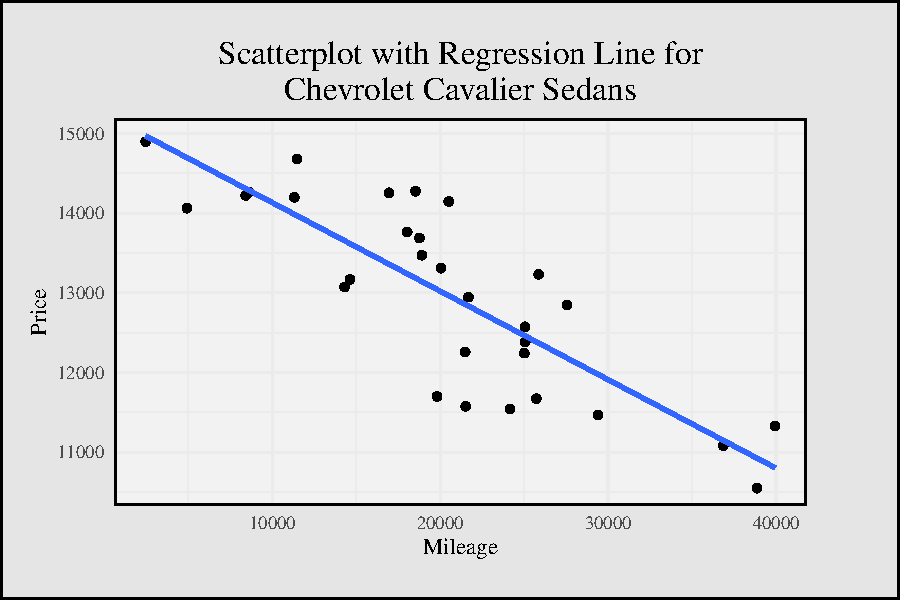
\includegraphics{Chap3_files/figure-latex/df_1-plot-1.pdf}
\caption{(\#fig:df\_1-plot)Scatterplot and regression line for Chevrolet Cavalier Sedans: Price = 15,244 - 0.111(Mileage).}
\end{figure}

Using our highlighted observation (11,488, 14,678.1), we see that
\begin{equation}
y_i - \bar{y} = (y_i - \hat{y}_i) + (\hat{y}_i - \bar{y}) \notag
\end{equation}
\begin{equation}
14{,}678.1 - 12{,}962 = (14{,}678.1 - 13{,}967.68) + (13{,}967.68 - 12{,}962) \notag
\end{equation}
\begin{equation}
1716.1 = 710.42 + 1005.68 \notag
\end{equation}

Squaring both sides of Equation (3.7) and then summing over all observations results in

\begin{align}
\sum_{i=1}^n (y_i - \bar{y})^2 \notag
  &= \sum_{i=1}^n (y_i - \hat{y}_i)^2
  + \sum_{i=1}^n (\hat{y}_i - \bar{y})^2
  + 2 \sum_{i=1}^n (\hat{y}_i - \bar{y})(y_i - \hat{y}_i) \\[6pt] \tag{3.8}
  &= \sum_{i=1}^n (y_i - \hat{y}_i)^2 + \sum_{i=1}^n (\hat{y}_i - \bar{y})^2 \\[6pt] \notag
\end{align}

The key point of the previous calculations is to show that the total variability in the response, \(\sum_{i=1}^n (y_i - \bar{y})^2\), can be decomposed into the following:

\begin{equation}
\text{Total sum of squares (SST) = Residual sum of squares (SSE) + Regression sum of squares (SSR)} \notag
\end{equation}

MATHEMATICAL NOTE\\
To show that Equation (3.8) is true, we can write
\begin{equation}
2 \sum_{i=1}^n (y_i - \hat{y}_i)(\hat{y}_i - \bar{y})
  = 2 \sum_{i=1}^n \hat{y}_i (y_i - \hat{y}_i)
  - 2 \bar{y} \sum_{i=1}^n (y_i - \hat{y}_i) \notag
\end{equation}

\begin{quote}
\textbf{MATHEMATICAL NOTE}\\
Recall that the sum of residuals, \(\sum_{i=1}^n (y_i - \hat{y}_i)\), equals zero. In addition, it can be shown that the sum of the residuals, weighted by the corresponding predicted value, always sums to zero: \(\sum_{i=1}^n \hat{y}_i (y_i - \hat{y}_i) = 0.\) (See Questions 25 through 29.)
\end{quote}

\hypertarget{extended-activity-a-closer-look-at-least-squares-regression-equations}{%
\subsection*{Extended Activity: A Closer Look at Least Squares Regression Equations}\label{extended-activity-a-closer-look-at-least-squares-regression-equations}}
\addcontentsline{toc}{subsection}{Extended Activity: A Closer Look at Least Squares Regression Equations}

Data set: \(Cavalier\)\\
Note that calculus is required for Activity Questions 25 through 29.

\begin{enumerate}
\def\labelenumi{\arabic{enumi}.}
\setcounter{enumi}{21}
\tightlist
\item
  Create a regression model to predict Price from Mileage for the Cavalier data. Calculate the total sum of squares (SST), residual sum of squares (SSE), and regression sum of squares (SSR). Verify that SST = SSE + SSR.\\
\item
  Show that \(\sum_{i=1}^n (y_i - \hat{y}_i)(\hat{y}_i - \bar{y}) = 0\) for the model given in the previous question.\\
\item
  Using your final model in Question 21, calculate the total sum of squares (SST), residual sum of squares (SSE), and regression sum of squares (SSR). Verify that SST = SSE + SSR.\\
\item
  Set the partial derivative of the residual sum of squares with respect to \(b_0\) to zero, to show that \(b_0 n + b_1 \sum_{i=1}^n x_i = \sum_{i=1}^n y_i.\)
\item
  Set the partial derivative of the residual sum of squares with respect to \(b_1\) to zero, to show that \(b_0 \sum_{i=1}^n x_i + b_1 \sum_{i=1}^n x_i^2 = \sum_{i=1}^n x_i y_i.\)
\item
  The equations in Questions 25 and 26 are called the normal equations for simple linear regression. Use the normal equations to derive the least squares regression coefficients, \(b_0\) and \(b_1\).\\
\item
  Use the fact that \(\sum_{i=1}^n (y_i - \hat{y}_i) = 0\) and \(\hat{y}_i = b_0 + b_1 x_i\) to show that
  \begin{equation}
  \sum_{i=1}^n \hat{y}_i (y_i - \hat{y}_i)
    = b_1 \Bigl(\sum_{i=1}^n x_i y_i - b_0 \sum_{i=1}^n x_i - b_1 \sum_{i=1}^n x_i^2\Bigr). \notag
  \end{equation}
\item
  Use Questions 26 and 28 to show that \(\sum_{i=1}^n \hat{y}_i (y_i - \hat{y}_i) = 0.\)
\end{enumerate}

\hypertarget{the-analysis-of-variance-table}{%
\subsection{The Analysis of Variance Table}\label{the-analysis-of-variance-table}}

The objective of regression is to create a model that best fits the observed points. Least squares regression models define a ``best fit'' as a model that minimizes the sum of squared residual values, \(\sum_{i=1}^n (y_i - \hat{y}_i)^2\).

The coefficient of determination, \(R^2\), is the percentage of variation in the response variable that is explained by the regression line:

\begin{quote}
\textbf{KEY CONCEPT}\\
The coefficient of determination, \(R^2\), is a measure of the usefulness of the explanatory variables in the model. If the explanatory variables are useful in predicting the response, the residual sum of squares, \(\sum_{i=1}^n (y_i - \hat{y}_i)^2\), is small compared to the total spread of the responses, \(\sum_{i=1}^n (y_i - \bar{y})^2\). In other words, the amount of variability explained by the regression model, \(\sum_{i=1}^n (\hat{y}_i - \bar{y})^2\), is a large proportion of the total variability of the responses.
\end{quote}

The sum of squares calculations are often summarized in an analysis of variance (ANOVA) table, as shown in Table 1.

\begin{table}

\caption{\label{tab:anova-table}ANOVA table for a least squares regression model, where n is the number of observations and p is the number of terms in the model (including the constant term).}
\centering
\begin{tabular}[t]{l|c|c|c|c}
\hline
Source & df & SS & MS & F.Statistic\\
\hline
Regression & $\quad p - 1$ & $\displaystyle SSR = \sum_{i=1}^n (\hat{y}_i - \bar{y})^2$ & $MS_{Regr} = \tfrac{SSR}{df_{Regr}}$ & $F = MS_{Regr}/MSE$\\
\hline
Error & $\quad n - p$ & $\displaystyle SSE = \sum_{i=1}^n (y_i - \hat{y}_i)^2$ & $MSE = \tfrac{SSE}{df_{Error}} = \hat{\sigma}^2$ & \\
\hline
Total & $\quad n - 1$ & $\displaystyle SST = \sum_{i=1}^n (y_i - \bar{y})^2$ &  & \\
\hline
\end{tabular}
\end{table}

\hypertarget{testing-the-significance-of-a-regression-model}{%
\subsection{Testing the Significance of a Regression Model}\label{testing-the-significance-of-a-regression-model}}

Once a model has been developed, we are often interested in testing if there is a relationship between the response and the set of all explanatory terms in the model. To conduct an overall test of model adequacy, we test the following null and alternative hypotheses:

Notice that the \(\beta_0\) term in our regression model is not included in the null or the alternative hypothesis. Table 1 provides the details for the calculation of the F-statistic:
\begin{equation}
F = \frac{MS_{Regr}}{MSE}
  = \frac{SSR/(p - 1)}{SSE/(n - p)}
\tag{3.11}
\end{equation}

This statistic follows an \(F_{p-1,\,n-p}\) distribution, where \(n\) is the number of observations and \(p\) is the number of terms in the model (including \(\beta_0\)). The same assumptions about the error terms, \(\epsilon_i \overset{\mathrm{iid}}{\sim}N(0,\sigma^2)\), need to be checked before conducting the hypothesis test.

NOTE\\
There are no model assumptions needed about the error terms to calculate estimates of the coefficients. However, all the model assumptions should be checked before conducting a hypothesis test.

\hypertarget{the-extra-sum-of-squares-f-test}{%
\subsection{\texorpdfstring{The Extra Sum of Squares \(F\)-Test}{The Extra Sum of Squares F-Test}}\label{the-extra-sum-of-squares-f-test}}

We are often interested in testing the contribution of a particular variable (or subset of variables) to the regression sum of squares. The \textbf{extra sum of squares \(F\)-test} can test the contribution of a specific set of variables by comparing the residuals of a full and a reduced model.

Suppose a model has been fit with \(k\) terms---we call this a \textbf{full model}. We may hypothesize that only \(p < k\) terms really contribute to the regression model---we call this smaller model the \textbf{reduced model}. In this situation, we want to test whether

The previous ANOVA \(F\)-test can be modified to provide an \(F\)-test for this hypothesis. Notice that this hypothesis test makes no assumptions about the other terms, \(\beta_0, \beta_1, \dots, \beta_{p-1}\), in the model. In addition, \emph{every term in the reduced model must also be in the full model}.

This statistic follows an F-distribution with \(k-p\) and \(n-k\) degrees of freedom. The extra sum of squares \(F\)-test determines whether the difference between the sum of squared residuals in the full and reduced
models is so large that it is unlikely to occur by chance.

\hypertarget{extended-activity-testing-multiple-coefficients}{%
\subsection*{Extended Activity: Testing Multiple Coefficients}\label{extended-activity-testing-multiple-coefficients}}
\addcontentsline{toc}{subsection}{Extended Activity: Testing Multiple Coefficients}

Data set: \(Cavalier\)
Consider the Cavalier data set and the regression model \(y = \beta_0 + \beta_1(Mileage) + \beta_2(Cruise) + \epsilon\)\\
30. Submit the ANOVA table, \(F\)-statistic, and \(p\)-value to test the hypothesis \(H_0: \beta_1 = \beta_2 = 0\) versus \(H_a\): at least one of the coefficients is not 0.\\
31. Conduct an extra sum of squares test to determine if \(Trim\) is useful. More specifically, use the reduced model in the previous question and the full model
\begin{equation}
y = \beta_0 + \beta_1(\text{Mileage}) + \beta_2(\text{Cruise}) + \beta_3(\text{LS Sport Sedan 4D}) + \beta_4(\text{Sedan 4D}) \notag
\end{equation}
to test the hypothesis \(H_0: \beta_3 = \beta_4 = 0\) versus \(H_a\): at least one of the coefficients is not 0.

\begin{center}\rule{0.5\linewidth}{0.5pt}\end{center}

\hypertarget{developing-a-model-to-confirm-a-theory}{%
\section{3.9 Developing a Model to Confirm a Theory}\label{developing-a-model-to-confirm-a-theory}}

If the goal is to confirm a theoretical relationship, statisticians tend to go through the following steps to identify an appropriate theoretical model.

\(\bullet\) Verify that the response variable provides the information needed to address the question of interest. What are the range and variability of responses you expect to observe? Is the response measurement precise enough to address the question of interest?
\(\bullet\) Investigate all explanatory variables that may be of importance or could potentially influence your results. Note that some terms in the model will be included even though the coefficients may not be significant. In most studies, there is often prior information or a theoretical explanation for the relationship between explanatory and response variables. Nonstatistical information is often essential in developing good statistical models.\\
\(\bullet\) For each of the explanatory variables that you plan to include in the model, describe whether you would expect a positive or negative correlation between that variable and the response variable.\\
\(\bullet\) Use any background information available to identify what other factors are assumed to be controlled within the model. Could measurements, materials, and the process of data collection create unwanted variability? Identify any explanatory variables that may influence the response; then determine if information on these variables can be collected and if the variables can be controlled throughout the study. For example, in the Kelley Blue Book data set, the condition of the car was assumed to be the same for all cars. The data were collected for GM cars with model year 2005. Since these cars were relatively new and the cars were considered to be in excellent condition, any model we create for these data would not be relevant for cars that had been in any type of accident.\\
\(\bullet\) What conditions would be considered normal for this type of study? Are these conditions controllable? If a condition changed during the study, how might it impact the results?

After a theoretical model is developed, regression analysis is conducted one time to determine if the data support the theories.

KEY CONCEPT\\
The same data should not be looked at both to develop a model and to test it.

\hypertarget{extended-activity-testing-a-theory-on-cars}{%
\subsection*{Extended Activity: Testing a Theory on Cars}\label{extended-activity-testing-a-theory-on-cars}}
\addcontentsline{toc}{subsection}{Extended Activity: Testing a Theory on Cars}

Data set: \(Cars\)\\
Assume that you have been asked to determine if there is an association between each of the explanatory
variables and the response in the \(Cars\) data set.

\begin{enumerate}
\def\labelenumi{\arabic{enumi}.}
\setcounter{enumi}{31}
\item
  Use any background information you may have (not the \emph{Cars} data set) to predict how each explana-
  tory variable (except \(Model\) and \(Trim\)) will influence \(TPrice\). For example, will \(Liter\) or \(Mileage\)
  have a positive or negative association with \(TPrice\)? List each \(Make\) and identify which will impact
  \(TPrice\) most and in which direction.
\item
  Identify which factors are controlled in this data set. Can you suggest any factors outside the pro-
  vided data set that should have been included? If coefficients are found to be significant (have small
  \(p\)-values), will these relationships hold for all areas in the United States? Will the relationships hold for 2004 or 2001 cars?
\item
  Run a regression analysis to test your hypothesized model. Which variables are important in your model? Did you accurately estimate the direction of each relationship? Note that even if a variable is not significant, it is typically kept in the model if there is a theoretical justification
  for it.
\end{enumerate}

\begin{center}\rule{0.5\linewidth}{0.5pt}\end{center}

\hypertarget{interaction-and-terms-for-curvature}{%
\subsection{Interaction and Terms for Curvature}\label{interaction-and-terms-for-curvature}}

In addition to using the variables provided in a data set, it is often beneficial to create new variables that are functions of the existing explanatory variables. These new explanatory variables are often quadratic (\(X^2\)), cubic (\(X^3\)), or a product of two explanatory variables (\(X_1*X_2\)), called interaction terms.

An \textbf{interaction} is present if the effect of one variable, such as \(Mileage\), depends on a second variable, such as \(Cyl\). If an interaction exists, the influence of \(Cyl\) changes for different \(Mileage\) values, and also the influence of \(Mileage\) will depend on \(Cyl\).

The data set \(4-8Cyl\) includes several four- and eight-cylinder cars from the original Cars data. Figure 2 shows a scatterplot and regression line to predict \(Price\) using both \(Mileage\) and \(Cyl\). The regression model in Figure 2 has no interaction term. The parallel lines show that the estimated impact of changing cylinder size does not depend on mileage. Thus, for any given number of miles, when the number of cylinders changes from four to eight, we expect an increase in Price of \(4 \times 3443 = 13{,}772\).

In the same way, the \(Mileage\) coefficient states that holding \(Cyl\) constant, we expect \(Price\) to decrease by \(0.20\) for each additional mile on the car.

\begin{figure}
\centering
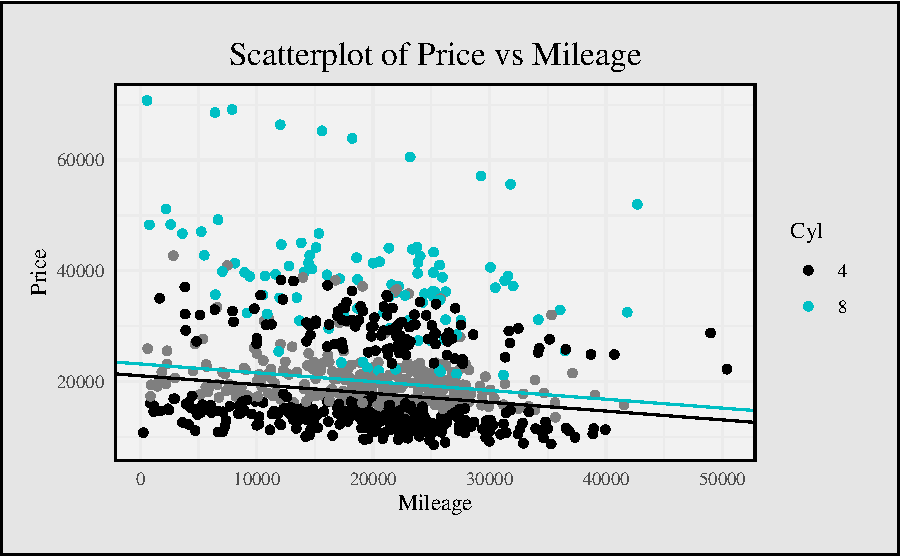
\includegraphics{Chap3_files/figure-latex/df_2-plot-1.pdf}
\caption{(\#fig:df\_2-plot)Scatterplot and least squares regression line: Price = 15,349 - 0.20(Mileage) + 3443(Cyl). For each cylinder size, an increase of one mile is expected to reduce price by \$0.20.}
\end{figure}

Figure 3 shows a scatterplot and regression line to predict \(Price\) using \(Mileage\), \(Cyl\), and a \(Mileage*Cyl\) interaction term (called \(MileCyl\)). The lack of parallel lines in the regression model \(\text{Price} = 4533 + 0.340(\text{Mileage}) + 5431(\text{Cyl}) - 0.0995(\text{MileCyl})\) indicates an interaction effect.

Caution should be used in interpreting coefficients when interaction terms are present. The coefficient for \(Mileage\) can no longer be globally interpreted as reducing \(Price\) by \(0.20\) for each additional mile. Now, when there are four cylinders, \(Price\) is reduced by \(0.058\ [0.340(1) - 0.0995(1 \times 4) = -0.058]\) with each additional mile. When there are eight cylinders, \(Price\) is reduced by \(0.456\ [0.340(1) - 0.0995(1 \times 8) = -0.456]\) with each additional mile. Thus, an additional mile impacts \(Price\) differently depending on the second variable, \(Cyl\).

\begin{figure}
\centering
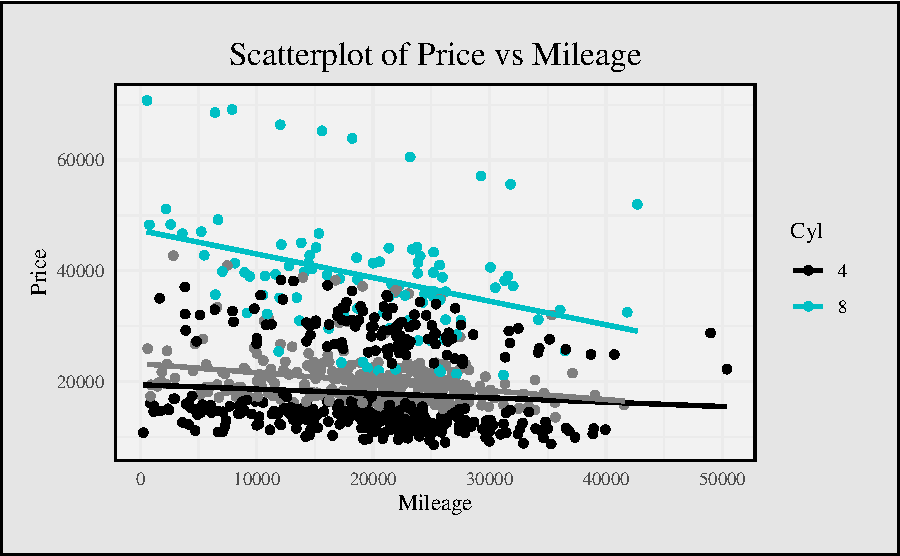
\includegraphics{Chap3_files/figure-latex/df_3-plot-1.pdf}
\caption{(\#fig:df\_3-plot)Scatterplot and and least squares regression line: Price = 4533 + 0.340(Mileage) + 5431(Cyl) + 0.0995(MileCyl). If the interaction term (MileCyl) is important, we expect to have regression lines that are not parallel.}
\end{figure}

\vspace*{2cm}

\hypertarget{extended-activity-understanding-interaction-terms}{%
\subsection*{Extended Activity: Understanding Interaction Terms}\label{extended-activity-understanding-interaction-terms}}
\addcontentsline{toc}{subsection}{Extended Activity: Understanding Interaction Terms}

Data set: \(4-8Cyl\)

\begin{enumerate}
\def\labelenumi{\arabic{enumi}.}
\setcounter{enumi}{34}
\tightlist
\item
  Use the \(4-8Cyl\) data set to calculate the two regression equations shown in Figures 2 and 3.
\end{enumerate}

\begin{enumerate}
\def\labelenumi{\alph{enumi}.}
\tightlist
\item
  Does the \(R^2_{\text{adj}}\) value increase when the interaction term is added? Based on the change in \(R^2_{\text{adj}}\), should the interaction term be included in the model?
\item
  For both models, calculate the estimated price of a four-cylinder car when \(Mileage\) = 10,000.
\item
  Assuming \(Mileage\) = 10,000, for both models explain how increasing from four to eight cylinders will impact the estimated price.
\item
  Conduct an extra sum of squares test to determine if the \(MileCyl\) interaction term is important to the model.
\end{enumerate}

\begin{enumerate}
\def\labelenumi{\arabic{enumi}.}
\setcounter{enumi}{35}
\tightlist
\item
  Use the \(4-8Cyl\) data set to calculate the regression line \(Price = \beta_0 + \beta_1(Mileage) + \beta_3(Cadillac) + \beta_4(SAAB)\). You will need to create indicator variables for \(Make\) before calculating the regression line.
\end{enumerate}

\begin{enumerate}
\def\labelenumi{\alph{enumi}.}
\tightlist
\item
  Create a scatterplot with \(Mileage\) as the explanatory variable and \(Price\) as the response. Overlay a second graph with \(Mileage\) as the explanatory variable and \(\hat y\) as the response. Notice that the predicted values (the \(\hat y\) values) form two separate lines. Do the parallel lines (no interaction model) look appropriate?
\item
  Conduct one extra sum of squares test to determine if interaction terms (\(MileCadillac\) and \(MileSAAB\)) are important to the model (i.e., test the hypothesis \(H_0: \beta_5 = \beta_6 = 0\) versus \(H_a\): at least one of the coefficients is not 0, where \(\beta_5\) and \(\beta_6\) are the coefficients for the two interaction terms). Create a scatterplot with the full regression model to explain the results of the hypothesis test.
\end{enumerate}

\hypertarget{quadratic-and-cubic-terms}{%
\subsection{Quadratic and Cubic Terms}\label{quadratic-and-cubic-terms}}

If a plot of residuals versus an explanatory variable shows curvature, the model may be improved by including a quadratic term. Is the relationship between mileage and retail price linear or quadratic for the Kelley Blue Book data? To test this, a quadratic term \(Mileage*Mileage\) can be created and included in a regression model.

\begin{quote}
\textbf{MATHEMATICAL NOTE}\\
Even though models with quadratic (\(x^2\)) or cubic (\(x^3\)) terms are not linear functions of the original explanatory variables, the mean response is linear in the regression coefficients (\(\beta_0, \beta_1, \beta_2, \dots\)). For example \(y = \beta_0 + z_1 \beta_1 + z_2 \beta_2 + \epsilon\) would be considered a linear regression model when \(z_1 = x\) and \(z_2 = x^2\).
\end{quote}

\hypertarget{extended-activity-understanding-quadratic-terms}{%
\subsection*{Extended Activity: Understanding Quadratic Terms}\label{extended-activity-understanding-quadratic-terms}}
\addcontentsline{toc}{subsection}{Extended Activity: Understanding Quadratic Terms}

Data set: \(MPG\)
The MPG data compare the miles per gallon of several cars against the speed the car was going as well as displacement. Displacement is a measure of the volume of all the cylinders within an engine. The larger the displacement, the more quickly fuel can move through an engine, giving the vehicle more power.

\begin{enumerate}
\def\labelenumi{\arabic{enumi}.}
\setcounter{enumi}{36}
\tightlist
\item
  Use the \(MPG\) data to create a regression model to predict \(MPG\) from \(Speed\) and \(Displacement\): \(\mathrm{MPG} = \beta_0 + \beta_1(\mathrm{Speed}) + \beta_2(\mathrm{Displacement}).\)
\end{enumerate}

\begin{enumerate}
\def\labelenumi{\alph{enumi}.}
\tightlist
\item
  What are the regression equation and \(R^2\) value?
\item
  Look at residual versus \(Speed\) and residual versus \(Displacement\) plots. Describe any patterns you see.
\item
  What does the residual normal probability plot show?
\end{enumerate}

\begin{enumerate}
\def\labelenumi{\arabic{enumi}.}
\setcounter{enumi}{37}
\tightlist
\item
  Create a regression model to predict \(MPG\) from Speed: \(\mathrm{MPG} = \beta_0 + \beta_1(\mathrm{Speed}).\)
\end{enumerate}

\begin{enumerate}
\def\labelenumi{\alph{enumi}.}
\tightlist
\item
  What are the regression equation and \(R^2\) value?
\item
  Look at residual versus \(Speed\) and residual versus \(Displacement\) plots. Describe any patterns in the residual plots.
\item
  Describe any patterns in the residual normal probability plot.
\item
  Is \(Displacement\) an important explanatory variable? Use the residual plots and \(R^2\) to give an intuitive explanation.
\end{enumerate}

\begin{enumerate}
\def\labelenumi{\arabic{enumi}.}
\setcounter{enumi}{38}
\tightlist
\item
  Create a model using displacement to predict \(MPG\): \(\mathrm{MPG} = \beta_0 + \beta_1(\mathrm{Displacement}).\)
\end{enumerate}

\begin{enumerate}
\def\labelenumi{\alph{enumi}.}
\tightlist
\item
  What are the regression equation and \(R^2\) value?
\item
  Look at residual versus \(Speed\) and residual versus \(Displacement\) plots. Describe any patterns in the residual plots.
\end{enumerate}

\begin{enumerate}
\def\labelenumi{\arabic{enumi}.}
\setcounter{enumi}{39}
\tightlist
\item
  Create a (\(\mathrm{Speed}\))\^{}2 term (called \(Speed_Sq\)) and incorporate that term into your regression model to predict \(MPG\): \(\mathrm{MPG} = \beta_0 + \beta_1(\mathrm{Speed}) + \beta_2(\mathrm{Displacement}) + \beta_3(\mathrm{Speed\_Sq}).\)
\end{enumerate}

\begin{enumerate}
\def\labelenumi{\alph{enumi}.}
\tightlist
\item
  What are the regression equation and \(R^2\) value?
\item
  Look at residual versus \(Speed\) and residual versus \(Displacement\) plots. Describe any changes when (\(\mathrm{Speed}\))\^{}2 is added to the model.
\item
  What does the residual normal probability plot show?
\end{enumerate}

\hypertarget{extended-activity-creating-new-terms-to-predict-the-retail-price-of-cars}{%
\subsection{Extended Activity: Creating New Terms to Predict the Retail Price of Cars}\label{extended-activity-creating-new-terms-to-predict-the-retail-price-of-cars}}

Data set: \(Cars\)
The potential outliers identified in Question 11 can provide an interesting demonstration of an interaction. Figure 3.12 shows that the slope to predict \(Price\) from \(Mileage\) for the ten Cadillac XLR-V8s is much steeper than the slope found when using the other cars. This shows that depreciation for these high-end cars is almost 50 cents a mile, as opposed to 15 cents a mile on average for all car types combined.

\begin{figure}
\centering
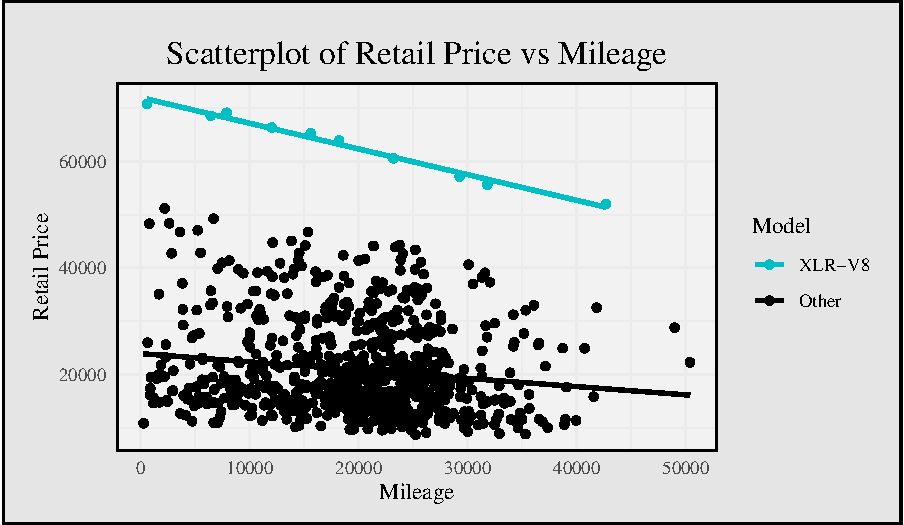
\includegraphics{Chap3_files/figure-latex/df_4-plot-1.pdf}
\caption{(\#fig:df\_4-plot)Scatterplot and regression lines: For the Cadillac XLR-V8, the regression line is Price = 71,997 - 0.4827(Mileage). This is a much steeper line than the regression line for all other cars: Price = 23,894 - 0.1549(Mileage).}
\end{figure}

\begin{enumerate}
\def\labelenumi{\arabic{enumi}.}
\setcounter{enumi}{40}
\tightlist
\item
  Create a quadratic mileage term. Create two models to predict \(TPrice\), one with only \(Mileage\) and another with both \(Mileage\) and \((Mileage)^2\) (called \(MileSq\)).
\end{enumerate}

\begin{enumerate}
\def\labelenumi{\alph{enumi}.}
\tightlist
\item
  How much does the \(R^2\) value increase if a quadratic term is added to the model \(TPrice = \beta_0 + \beta_1(Mileage)\)?
\item
  Look at plots of residuals versus \(Mileage\) in both models. Did the addition of the \(MileSq\) term improve the residual plots?
\end{enumerate}

\begin{enumerate}
\def\labelenumi{\arabic{enumi}.}
\setcounter{enumi}{41}
\item
  Create an interaction term \(Mileage*Cyl\) (called \(MileCyl\)). Use \(Mileage\), \(Cyl\), and \(MileCyl\) to predict \(Price\). Does this interaction term appear to improve the model? Use residual plots and \(R^2\) to justify your answer.\\
  While there is no ``best'' model, many final models developed by students in Question 21 tend to include the terms \(Cadillac\), \(Convertible\), and \(Liter\). Since each of these terms is related to the Cadillac XLR-V8, it may be helpful to include an interaction term for \(Mileage*Cadillac\), \(Mileage*Convertible\), or \(Mileage*Liter\). Other \(Mileage\), \(Make\), or \(Type\) interactions may also be helpful additions to the model.
\item
  Develop additional quadratic and interaction terms. Determine if they improve the regression model in Question 42.
\item
  Submit a new regression model that best predicts \(TPrice\). Does including quadratic or interaction terms improve your model from what was developed in Question 21?
\end{enumerate}

Unless there is a clear reason to include them, researchers typically do not create interaction terms and test whether they should be included in a model. Most of the researcher's effort should be spent on determining whether the original explanatory variables provided in the data set are related to the response. If an interaction term (\(X_i * X_j\)) is included in a final model, it is common practice to include each of the original terms (\(X_i\) and \(X_j\)) in the model as well (even if the coefficients of the original terms are close to zero).

\begin{center}\rule{0.5\linewidth}{0.5pt}\end{center}

\hypertarget{a-closer-look-at-variable-selection-criteria}{%
\section{3.11 A Closer Look at Variable Selection Criteria}\label{a-closer-look-at-variable-selection-criteria}}

The growing number of large data sets as well as increasing computer power has dramatically improved the ability of researchers to find a \textbf{parsimonious model} (a model that carefully selects a relatively small number of the most useful explanatory variables). However, even with intensive computing power, the process of finding a ``best'' model is often more of an art than a science.

As shown earlier, stepwise procedures that use prespecified conditions to automatically add or delete variables can have some limitations:

\(\bullet\) When explanatory variables are correlated, stepwise procedures often fail to include variables that are useful in describing the results.\\
\(\bullet\) Stepwise procedures tend to overfit the data (fit unhelpful variables) by searching for any terms that explain the variability in the sample results. This chance variability in the sample results may not be reflected in the entire population from which the sample was collected.\\
\(\bullet\) The automated stepwise process provides a ``best'' model that can be easily misinterpreted, since it doesn't require a researcher to explore the data to get an intuitive feel for the data. For example, stepwise procedures don't encourage researchers to look at residual plots that may reveal interesting patterns within the data.

\#\#\$ Adjusted \(R^2\)

While \(R^2\) is useful in determining how well a particular model fits the data, it is not very useful in variable selection. Adding new explanatory variables to a regression model will never increase the residual sum of squares; thus, \(R^2\) will increase (or stay the same) even when an explanatory variable does not contribute to the fit.

The \textbf{adjusted} \(R^2\) (\(R^2_{adj}\)) increases only if the improvement in model fit outweighs the cost of adding an additional term in the model:
\begin{equation}
R^2_{adj} = 1 - \left(\frac{n - 1}{n - p}\right)\frac{\sum_{i=1}^n (y_i - \hat{y}_i)^2}{\sum_{i=1}^n (y_i - \bar{y})^2}
= 1 - \left(\frac{n - 1}{n - p}\right)(1 - R^2)
\tag{3.13}
\end{equation}
where \(n\) is the sample size and \(p\) is the number of coefficients in the model (including the constant term).

\begin{quote}
\#\#MATHEMATICAL NOTE\#\#\\
Intuitively, each additional term in a regression model means that one additional parameter value must be estimated. Each parameter estimate costs an additional degree of freedom. Thus, \(R^2_{adj}\) is an \(R^2\) value that is adjusted for degrees of freedom and can be written as
\begin{equation}
R^2_{adj} = 1 - \frac{\text{MSE}}{\text{SST}/(n - 1)} \notag
\end{equation}
\(R^2_{adj}\) measures the spread of the residuals using MSE, while \(R^2\) measures the spread of the residuals using SSE.
\end{quote}

\hypertarget{mallows-c_p}{%
\subsection{\texorpdfstring{Mallows' \(C_p\)}{Mallows' C\_p}}\label{mallows-c_p}}

Another approach to variable selection is to use Mallows' \(C_p\) statistic:
\begin{equation}
C_p = (n - p)\left(\frac{\hat{\sigma}^2}{\hat{\sigma}^2_{Full}}\right) + (2p - n)
= (n - p)\left(\frac{MSE}{MSE_{Full}}\right) + (2p - n)
\tag{3.14}
\end{equation}

where \(n\) is the sample size, \(p\) is the number of coefficients in the model (including the constant term), \(\hat{\sigma}^2\) estimates the variance of the residuals in the model, and \(\hat{\sigma}^2_{Full}\) estimates the variance of the residuals in the full model (i.e., the model with all potential explanatory variables in the data set).

If the current model lacks an important explanatory variable, \(\hat{\sigma}^2\) is much larger than \(\hat{\sigma}^2_{Full}\) and \(C_p\) tends to be large. For any models where \(\hat{\sigma}^2\) is similar to \(\hat{\sigma}^2_{Full}\), \(C_p\) provides a penalty, \(2p - n\), to favor models with a smaller number of terms. For a fixed number of terms, minimizing \(C_p\) is equivalent to minimizing SSE, which is also equivalent to maximizing \(R^2\).

The \(C_p\) statistic assumes that \(\hat{\sigma}^2_{Full}\) is an unbiased estimate of the overall residual variability, \(\sigma^2\). If the full model has several terms that are not useful in predicting the response (i.e., several coefficients are essentially zero), then \(\hat{\sigma}^2_{Full}\) will overestimate \(\sigma^2\) and \(C_p\) will be small.*

When the current model explains the data as well as the full model, \(\hat{\sigma}^2 / \hat{\sigma}^2_{Full} = 1\). Then \(C_p = (n - p)(1) + 2p - n = p\) Thus, the objective is often to find the smallest \(C_p\) value that is close to p.

\hypertarget{akaikes-information-criterion-aic-and-bayes-information-criterion-bic}{%
\subsection{Akaike's Information Criterion (AIC) and Bayes' Information Criterion (BIC)}\label{akaikes-information-criterion-aic-and-bayes-information-criterion-bic}}

Two additional model selection criteria are the Akaike information criterion (AIC) and the Bayesian information criterion (BIC).† Both of these criteria are popular because they are also applicable to regression models fit by maximum likelihood techniques (such as logistic regression), whereas \(R^2\) and \(C_p\) are appropriate only for least squares regression models.

Calculations for these two criteria are provided below. These statistics also include a measure of the variability of the residuals plus a penalty term:
\begin{equation}
AIC = n[\log(\hat{\sigma}^2)] + 2p \notag
\end{equation}
\begin{equation}
BIC = n[\log(\hat{\sigma}^2)] + p[\log(n)] \notag
\end{equation}

where \(n\) is the sample size, \(p\) is the number of coefficients in the model, and \(\hat{\sigma}^2\) estimates the variance of the residuals in the model.

AIC and BIC are identical except for their penalties, \(2p\) and \(p[\log(n)]\), respectively. Thus, AIC and BIC will tend to select slightly different models based on \(n\). AIC and BIC both select models that correspond to the smallest value.

KEY CONCEPT\\
No individual criterion (\(R^2_{adj}\), \(C_p\), AIC, or BIC) is universally better than the other selection criteria. While these tools are helpful in selecting models, they do not produce a model that is necessarily ``best.''

\hypertarget{model-validation}{%
\subsection{Model Validation}\label{model-validation}}

Often our goal is not just to describe the sample data, but to generalize to the entire population from which the sample was drawn. Even if a regression model is developed that fits the existing sample data very well and satisfies the model assumptions, there is no guarantee that the model will accurately predict new observations.

Variable selection techniques choose variables that account for the variation in the response. When there are many explanatory variables, it is likely that at least some of the terms selected don't explain patterns seen in the entire population; they are included simply because of chance variability seen in the sample.

To validate that a regression model is useful for predicting observations that were not used to develop
the model, do the following:

\(\bullet\) Collect new data from the same population as the original data. Use the new data to determine the
predictive ability of the original regression model.\\
\(\bullet\) Split the original data. For example, randomly select 75\% of the observations from the original data
set, develop a model, and check the appropriate model assumptions. Test the predictive ability of the
model on the remaining 25\% of the data set. This is often called \textbf{cross-validation}.\\
\(\bullet\) When the data set is not large enough to split, try \textbf{jackknife validation}. Hold out one observation at
a time, develop a model using the \(n-1\) remaining observations, and then estimate the value of the observation that was held out. Repeat this process for each of the n observations and calculate a predictive \(R^2\) value to evaluate the predictive ability of the model.\\
\(\bullet\) Use theory and prior experience to compare your regression model with other models developed with
similar data.

\hypertarget{chapter-summary__needs-several-tables}{%
\section{Chapter Summary\_\_{[}{[}{[}NEEDS SEVERAL TABLES{]}{]}{]}}\label{chapter-summary__needs-several-tables}}

In this chapter, we discussed techniques to describe, predict, and test hypotheses about the relationship
between a quantitative response variable and multiple explanatory variables. The goals of a regression model
will influence which techniques should be used and which conclusions can be drawn. The Cars activities
in this chapter focused on developing a model that could describe the relationship between the explanatory
variables and response variable as well as predict the value of the response based on a function of the explanatory variables.

Iterative techniques such as best subsets regression are often very useful in identifying which terms should be included in a model. The process of selecting explanatory variables to include in a model often involves iterative techniques, in which numerous models are created and compared at each step in the process. Iterative techniques should not be used when the goal of multiple regression is to test hypotheses. Stepwise regression is used to find the model with the highest R2 value; however, it does not provide much useful information about the model. For example, important variables (such as Liter in our investigation) are often not included in the stepwise regression models. Best subsets regression is a more useful iterative technique
because it allows the researcher to better identify important explanatory variables, even if multicollinearity (highly correlated explanatory variables) exists. Table 3.3 lists the key measures used in variable selection.

No individual criterion (\$\emph{\{R\^{}2\}}\{adj\}, \(C_p\), \(AIC\), or \(BIC\)) is universally better than the other selection criteria. These tools are helpful in selecting models, but they do not produce a model that is necessarily ``best.''

While iterative techniques are useful in reducing a large number of explanatory variables to a more manageable set, a researcher should ask the following questions to evaluate the resulting model:

\begin{itemize}
\tightlist
\item
  Were the techniques used to create the model appropriate based on the goals of the regression model?
\item
  Do the coefficients make sense? Are the magnitudes of the coefficients reasonable? If the coefficients have the opposite sign than expected, multicollinearity may be present, the range of the explanatory variables may be too small, or important explanatory variables may be missing from the model.
\item
  Do the residual plots identify any outliers or patterns that indicate unexplained structure that should be included in the model?
\end{itemize}

If the goal is to use hypothesis testing to determine how each of the explanatory variables impacts the response, iterative techniques are not appropriate. In addition, hypothesis tests about specific explanatory variables are not reliable when multicollinearity or lack of normality exists.

Model assumptions need to be met if the goal is to test hypotheses. While least squares regression models can be calculated without checking model assumptions, identifying patterns in residual plots that may indicate heteroskedasticity, autocorrelation, outliers, or lack of normality is important to creating a good model.

If a pattern exists in any of the residual plots, it is likely that another model exists that better explains the response variable. Researchers need to be somewhat creative in deciding which graphs to create and how to adapt a model based on what they see.

{[}{[}{[}Table 3.3{]}{]}{]}

\#\#\#\#\#CHAPTER 2\#\#\#\#\#\#\#\#\#\#\#\#\#\#\#\#\#

\begin{quote}
\textbf{Note}
Throughout this chapter, \(\bar{y}_{1.} = \bar{y}_{1}\) and \(\bar{y}_{2.} = \bar{y}_{2}\). The dot notation is often used with more complex models
to indicate that the average was taken over all values of that subscript. For example, \(bar{y}_{2.}\) averages over all
\(j = 1, 2, 3, ... , n_2\), observations from the standard game sample results.
\end{quote}

The effect of the color distracter game, \(\alpha_1\) , can be estimated by \(\hat{\alpha}_1 = \bar{y}_{1.} - \bar{y}_{..}\). Similarly, \(\hat{\alpha}_2 = \bar{y}_{2.} - \bar{y}_{..}\)
estimates the standard game effect, \(\alpha_2\). As in regression and the two-sample t-test, each residual \(\hat{\epsilon}_{ij}\) is the
difference between an observed value and the corresponding mean response.

R2 \(R^2\)
X1 \(X_1\)
X2 \(X_2\)
p-values \(p\)-values
m1 \(\mu_1\)
m2 \(\mu_2\)
a1 \(\alpha_1\)
s2 \(\sigma^2\)

\hypertarget{the-design-and-analysis-of-factorial-experiments-microwave-popcorn}{%
\chapter{The Design and Analysis of Factorial Experiments: Microwave Popcorn}\label{the-design-and-analysis-of-factorial-experiments-microwave-popcorn}}

However beautiful the strategy, you should occasionally
look at the results.
--- Winston Churchill

Statistics ought to be viewed as a whole: understanding the process of formulating questions, properly designing a study, actively collecting meaningful data, and then deciding
how to properly organize and draw conclusions from the data. Advancements in technology have made data collection and computationally intensive statistical techniques much more
feasible. At one time, many statisticians had narrowly defined roles and were considered as
primarily ``number crunchers.'' Today, statisticians characteristically work on interdisciplinary
teams that emphasize scientific inference and understanding data in context.
Instead of emphasizing formulas, computation, and mathematical theory, this chapter
uses a simple popcorn experiment to demonstrate the numerous challenges that can occur in
designing experiments and collecting data.

The activities in this chapter will discuss the following:\\
\(\bullet\) Key features of a well-designed experiment and proper data collection.\\
\(\bullet\) Proper determination of response variables, experimental factors, and levels.\\
\(\bullet\) Building on the one-way ANOVA discussed in Chapter 2 to describe multivariate factorial designs.\\
\(\bullet\) Evaluating multiple hypotheses based on main effects and interaction terms.\\
\(\bullet\) Calculating each of the between-group and within-group variances needed in ANOVA tables for balanced factorial designs.\\
\(\bullet\) Calculating effects and developing mathematical models.\\
\(\bullet\) Using multiple comparison tests with ANOVA tables.

\hypertarget{investigation-which-microwave-popcorn-is-the-best}{%
\chapter{4.1 Investigation: Which Microwave Popcorn Is the Best?}\label{investigation-which-microwave-popcorn-is-the-best}}

Popcorn is a staple for many college students. While many students like popcorn because it is inexpensive
and easy to prepare, it is also a whole grain food that's low in fat and calories. According to The Popcorn
Institute, Americans consume an average of 54 quarts of popcorn a year per person.

Two popcorn lovers, who also happened to be taking a statistics course, decided to test whether there is a
difference in quality between microwave popcorn brands. Yvonne and Tue wanted to know if a cheaper brand
of popcorn was just as good as more expensive popcorn. These students could have chosen to conduct a study
that could be analyzed with a two-sample t-test if they had simply compared two brands of popcorn. However,
if they did a two-sample t-test, they would need to hold many factors constant, such as the type of microwave,
cooking time, and storage procedures. Since Yvonne and Tue believed that some of these factors could also
impact the quality of the popcorn, they decided to include some of these additional factors in their study.

Modeling real-world phenomena often requires more than just one factor to explain changes in the
response. \textbf{Factorial designs} are any statistical designs that are structured to use factors (i.e., explanatory
variables) to organize meaningful groups of treatment conditions. A two-sample t-test can be considered a
special case of a factorial design that has just one factor (popcorn brand in this case) and two levels (Brand A
and Brand B). Factorial designs are very powerful statistical tools because they allow a researcher to simul-
taneously test the effects of multiple factor-level combinations on a response of interest.

KEY CONCEPT\\
In factorial designs, each explanatory variable is called a \textbf{factor} and specific conditions within each
factor are called \textbf{levels}. In any study, these factor-level combinations are called \textbf{conditions}; in experi-
ments, they are often called \textbf{treatments}. Factorial designs are often used to test the effects of multiple
factors simultaneously, where each factor has two or more levels.

\hypertarget{elements-of-a-well-designed-experiment}{%
\chapter{4.2 Elements of a Well-Designed Experiment}\label{elements-of-a-well-designed-experiment}}

Unfortunately, many people mistakenly believe that statistics is only a process of performing mathematical
calculations on data in order to examine the validity of a hypothesis. Proper experimental design is just as
important as, if not more important than, the choice of statistical calculations. In fact, designing experi-
ments and collecting appropriate data are often the most difficult and time-consuming aspects of conducting
experiments.

KEY CONCEPT\\
A good design attempts to answer the question(s) of interest as clearly and efficiently as possible. Any
statistical analysis is only as good as the quality of the data.

An \textbf{experiment} is defined as a study in which purposeful changes are made to controlled conditions in
order to identify changes in a response. An experiment imposes a treatment on subjects or experimental units,
while an \textbf{observational study} simply collects data under varying conditions without imposing any changes.

Well-designed experiments are conducted under controlled conditions to make it easier to isolate the impact
of each treatment combination. In observational studies, the conditions in the study are rarely the only char-
acteristic that makes the two (or more) populations different. Thus, unknown factors that may bias the results
are unfortunately built into an observational study.

KEY CONCEPT\\
Both experiments and observational studies use sample data to draw conclusions about a larger
population, process, or system. It is often much easier to show cause and effect relationships in a
well-designed experiment because conditions are controlled.

NOTE
Some texts state that only experiments can be used to show cause and effect relationships. However, poorly
designed experiments should not be used to show causation. In addition, observational studies (such as
those testing a relationship between smoking and lung cancer) can be used to show causation if (1) there is
a strong association between the explanatory and response variables, (2) higher doses are associated with
stronger responses (e.g., more cigarettes increase the likelihood of getting cancer), (3) there are consistent
results across many studies, and (4) there are credible explanations for the cause and effect relationship.

\textbf{Experimental design} is the process of planning an experiment that collects the right amount and type
of data to answer a question of interest. Several decisions need to be made about how an experiment is to be
constructed and executed to ensure that the experimental results are valid. Taking the time to properly design
an experiment will improve the precision of answers to research questions. In addition, well-designed experi-
ments often are much more efficient and obtain stronger conclusions than other studies.

The first step in designing an experiment is to clearly define a problem and state the objectives of the
experiment. This is often much more difficult than it first appears. Before any data are collected, it is essential
that everyone involved understand the objectives of the experiment, what measurements will be taken, what
material is needed, and what procedures will be used. Good experimental design typically involves gaining
background knowledge outside the field of statistics.

There are many possible ways to conduct an experiment to determine the effect of brand on the quality
of popcorn. While microwave popcorn is something these students were quite familiar with, they needed to
determine which brands to compare, the appropriate cooking time (which could vary by microwave), and how
to define and measure ``good'' popcorn.

\hypertarget{identifying-a-response-variable}{%
\section{Identifying a Response Variable}\label{identifying-a-response-variable}}

Many possible measurements could be taken on microwave popcorn. Yvonne and Tue could have created a
taste rating or a texture rating, measured the volume of the kernels, counted the number of popped kernels, or
calculated the percentage of ``old maids,'' the kernels that did not pop after the bag had been cooked.

Identifying the response variable corresponds to determining what measurements should be taken. Each
experiment should ensure that the response variable provides the information needed and that the response
measurement is precise enough to address the question of interest. Yvonne and Tue determined that their
definition of ``quality'' popcorn would be popcorn that had the highest percentage of popped kernels per bag.
Notice that if Yvonne and Tue had counted only the popped kernels, and not the unpopped kernels, they might
have gotten a distorted response, since some brands may tend to have more kernels per bag.

Yvonne and Tue initially discussed randomly sampling 20 kernels from each popped bag and calculating the percentage of popped kernels. However, the size and shape differences between popped and
un-popped kernels would have made it rather difficult to simply pull out a random sample. Thus, in order
to ensure their counts were as accurate as possible, they decided to count every kernel in every bag of their
experiment.

It is also useful to discuss the range and variability of responses expected to be observed. For example,
if we conducted a study under conditions that typically gave only two outcomes, either 0\% or 100\%, the
response would be categorical (such as yes/no or popped/not popped), and then an analysis based on cat-
egorical response variables should be used. Studies with categorical response variables can be analyzed
with techniques such as the chi-square test or logistic regression, which are discussed in Chapters 6 and 7,
respectively.

The percentage of popped kernels was considered a quantitative response variable in this experiment.
Background research showed that some popcorn companies expected between 94\% and 97\% popped kernels,
but based on their prior popctorn eating experience, Yvonne and Tue expected the percentage to be a little
lower. In Yvonne and Tue's study, they roughly estimated that responses should be between 60\% and 99\%
popped kernels, with an average close to 90\%.

KEY CONCEPT\\
Care needs to be taken before a study is conducted to ensure that the response measurement is accu-
rate and applicable to the research question.

\hypertarget{identifying-the-factors-and-levels}{%
\section{Identifying the Factors and Levels}\label{identifying-the-factors-and-levels}}

The next step in designing an experiment is to investigate any factors that may be of importance or may
potentially bias the results. Yvonne and Tue had two microwaves that they typically used to make popcorn,
one in their dorm lounge and one in their room. The lounge microwave had a ``popcorn'' setting, which cooked
for 1 minute 45 seconds, though the package instructions for each brand suggested varying cooking times.
Most microwaves also have power settings. Should popcorn always be popped at the highest power setting?

With a little research, these students found that the quality of popcorn can also be affected by how it is
stored. Popcorn stored in a moisture-rich environment, such as a refrigerator, tends to have a higher percentage
of popped kernels. However, too much moisture may cause the popcorn to have a gummy texture. Finally,
Yvonne and Tue wanted to compare a relatively expensive brand of popcorn (Pop Secret) to a relatively
inexpensive brand (Fastco). Each of these brands also has a variety of flavors, such as butter, kettle corn, and
caramel.

Notice that the discussion of factors and potential levels is based not on statistical calculations, but on
nonstatistical knowledge. Nonstatistical knowledge is often essential in choosing factors, determining factor
levels, and interpreting the results of a study.

Yvonne and Tue decided on three factors of interest, factors that would be included in the study to
determine if different levels impact the results:\\
Factor 1: popcorn Brand at two levels, Fastco and Pop Secret\\
Factor 2: Microwave at two levels, Lounge and Room\\
Factor 3: cooking Time at two levels, 105 seconds and 135 seconds

It can sometimes be difficult to identify a reasonable range for each factor. Yvonne and Tue had noticed
that some brands of popcorn tended to burn at around 150 seconds (2.5 minutes). Even though cooking pop-
corn longer than 135 seconds might increase the percentage of popped kernels, Yvonne and Tue decided to
avoid cooking times likely to cause burning.

Yvonne and Tue then listed suspected extraneous variables, other factors that need to be controlled
during the experiment to eliminate potential biases. Yvonne and Tue decided to hold some extraneous vari-
ables constant. In particular, they used only the highest power setting on each microwave, they stored all
the popcorn on a shelf in their room, and they used only the butter flavor of each brand. There were other
variables they could not control, such as age of the popcorn, which manufacturing plant prepared each bag
of popcorn, and how different retail stores had stored the popcorn. To account for the extraneous variables
they could not control (or had not even thought of ), it would be best to randomly select bags of popcorn from
the entire population. Instead, Yvonne and Tue did their best to randomly select several bags of Fastco and
Pop Secret butter popcorn from a variety of stores in town. This was not a true random sample, and Yvonne
and Tue had to be careful in making any statements about how the results of their study extended to a larger
population. In addition, when possible, each bag of popcorn in the study was randomly allocated to a factor-
level combination. While bags of popcorn can be randomly assigned to a cooking time and microwave, they
cannot be randomly assigned to a popcorn brand.

KEY CONCEPT\\
A good design controls for known extraneous variables (often by holding them constant throughout
the study) and then uses random sampling and random allocation to control for any other unknown or
uncontrollable extraneous variables.

\hypertarget{choosing-a-design}{%
\section{Choosing a Design}\label{choosing-a-design}}

In addition to determining what conditions to test and what measurements to take, in order to create a good
experimental design, a researcher must properly define units and determine how units are structured. An
experimental unit is the smallest part of experimental material that is assigned (randomly, if possible) to a
factor-level combination within a study. Since Yvonne and Tue counted every kernel of popcorn, some may
incorrectly assume that each kernel is a unit. In an experiment, units are randomly assigned to treatments.
In this study, each kernel was not randomly assigned to a condition, but each bag of popcorn was randomly
assigned to be popped in a particular microwave for a particular length of time. Thus, bags of popcorn are
considered the units for Yvonne and Tue's study.

KEY CONCEPT\\
If (1) units are as similar as possible, (2) units are randomly assigned to treatment combinations, and
(3) large enough sample sizes are used, then we can conclude that statistically significant differences
in the response can be explained by the different treatment combinations.

This chapter will focus on \textbf{completely randomized factorial designs}. In completely randomized designs,
each unit is assigned to exactly one factor-level combination. Only one measurement is collected for each
unit. In the following section, we will use Yvonne and Tue's data to simultaneously test for the effects of two
brands, two cooking times, and two microwaves on the percentage of popped kernels.

NOTE\\
While this chapter focuses only on completely randomized factorial designs, it is important to recognize
the difference between completely randomized, \textbf{block} and \textbf{split-plot} or \textbf{(repeated measures) designs}.
If each unit is assigned to only one factor-level combination, it is appropriate to use a completely rand-
omized design. If each unit is assigned to several conditions or multiple measurements are taken on each
unit, a more complex design structure, such as a block or split-plot (repeated measures) design, may be
needed.
Block and split-plot (repeated measures) designs also work with different types of factors. The factors
of interest in this chapter all have fixed effects. \textbf{Fixed effects} correspond to factors where each level is
selected because it is of specific interest to the researcher. \textbf{Random effects} correspond to factors where
the levels are randomly selected from a larger population. All factors in a completely randomized design
are also \textbf{crossed}; this means that every level of each factor can be tested in combination with every
level of every other factor. Alternatively, \textbf{nested factors} are factors for which some levels cannot occur
simultaneously with other factor levels. Random effects and nested factors can be analyzed with block
and split-plot (repeated measures) designs; they are described in Chapter 5.

KEY CONCEPT\\
If possible, a straightforward design and analysis are usually better than a complex design and analy-
sis. If the design is too complicated and the data are not collected properly, even the most advanced
statistical techniques may not be able to draw appropriate conclusions from an experiment.

\hypertarget{determining-sample-sizes-for-completely-randomized-designs}{%
\section{Determining Sample Sizes for Completely Randomized Designs}\label{determining-sample-sizes-for-completely-randomized-designs}}

When more units are tested, it is more likely that the statistical analysis will identify true differences between
conditions. However, every unit tested has a cost, and it is important to carefully determine how many units are
practical to test. Is it worth testing additional units to gain a better understanding of the unit-to-unit variability?

Yvonne and Tue estimated that they could each count the kernels in one bag (popped and unpopped) in
10 to 15 minutes. They also thought that they could get a few close friends to count a few bags in exchange
for free popcorn. Care should always be taken when measuring results. If the result is a subjective measure-
ment (such as the taste of popcorn or the quality of artwork), very clear procedures should be written and, if
possible, the same people should record each measurement. In this popcorn study, counting the percentage of
popped kernels per bag is an objective measurement. As long as Yvonne and Tue have trustworthy friends,
there should be no problem in having several people help count popcorn kernels.* They estimated that they
could conduct 32 tests in about four hours.

The choice of 32 tests, instead of a round number like 30, is also related to a well-designed experiment.
Yvonne and Tue found that, based on their choice of factors and levels, there were a total of eight treatment
combinations. Table 4.1 lists the eight possible treatment conditions that can be ``assigned'' to each bag of
popcorn. Yvonne and Tue wanted to have a balanced design, a design where the same number of units is
assigned to (or randomly selected from) each condition. Balanced designs are often easier to analyze and more
likely to identify true differences in the effects of different conditions.3 If Yvonne and Tue wanted to conduct
a balanced design, they needed to conduct tests in a multiple of 8 (16, 24, etc.).

\hypertarget{table-4.1-treatment-combinations}{%
\subsection{Table 4.1: Treatment Combinations}\label{table-4.1-treatment-combinations}}

\begin{table}

\caption{(\#tab:table4.1)Table 4.1 All possible treatment conditions for the three‐factor popcorn study.}
\centering
\begin{tabular}[t]{cllr}
\toprule
Treatment Combination & Popcorn Brand & Microwave Location & Cooking Time\\
\midrule
1 & Fastco & Lounge & 105\\
2 & Pop Secret & Lounge & 105\\
3 & Fastco & Room & 105\\
4 & Pop Secret & Room & 105\\
5 & Fastco & Lounge & 135\\
\addlinespace
6 & Pop Secret & Lounge & 135\\
7 & Fastco & Room & 135\\
8 & Pop Secret & Room & 135\\
\bottomrule
\end{tabular}
\end{table}

MATHEMATICAL NOTE\\
Table 4.1 lists the variables in standard order. Listing conditions in \textbf{standard order} is a simple technique
that ensures that each factor combination is listed exactly once. The first variable alternates levels every
row. For the second variable, levels alternate every other row. The third variable alternates every fourth
row. This same process can work for multiple factors with multiple levels. If there were four factors, each
with two levels, the fourth column would alternate every eight rows. For studies with more than two levels,
simply ensure that the current variable lists each level exactly once for all prior combinations

\hypertarget{activity-determining-the-number-of-treatment-combinations}{%
\subsection{Activity: Determining the Number of Treatment Combinations}\label{activity-determining-the-number-of-treatment-combinations}}

\begin{enumerate}
\def\labelenumi{\arabic{enumi}.}
\tightlist
\item
  Assume we want to use three cooking times for popping the popcorn instead of two. List the possible
  treatment combinations that can be assigned. How many are there?\\
\item
  Without listing all possibilities, calculate how many treatment combinations would exist for a design
  that tested five brands with three microwaves at four cooking times.
\end{enumerate}

\hypertarget{analyzing-a-two-way-factorial-design}{%
\section{4.3 Analyzing a Two-Way Factorial Design}\label{analyzing-a-two-way-factorial-design}}

Since several factors are included in this experiment, there are also several hypotheses to be tested. Yvonne and Tue actually had six research questions, which will be discussed in Section 4.4. But to keep the calculations simple, in this section we will assume that only two factors were tested (\emph{Brand} and \emph{Time}). This leads to three hypotheses corresponding to the \emph{Brand} and \emph{Time} factors:

\begin{enumerate}
\def\labelenumi{\arabic{enumi}.}
\item
  \(H_{01}: \mu_{\text{Fastco}} = \mu_{\text{PopSecret}}\), there is no difference in the mean response (\emph{PopRate}) between the two \emph{Brands}.
  \(\quad H_{a1}: \mu_{\text{Fastco}} \neq \mu_{\text{PopSecret}}\), the two \emph{Brand} means are different.
\item
  \(H_{02}: \mu_{105} = \mu_{135}\), there is no difference in the mean \emph{PopRate} between the two \emph{Times}.
  \(\quad H_{a2}: \mu_{105} \neq \mu_{135}\), the two \emph{Time} means are different.
\item
  \(H_{03}:\) \emph{Brand} has no influence on how \emph{Time} affects \emph{PopRate}. This is equivalent to stating \(H_{03}:\) Time has no influence on how Brand affects PopRate or \(H_{03}:\) the effect of Time is the same for both Brands or \(H_{03}:\) there is no interaction between Time and Brand.\\
  \(H_{a3}:\) \emph{Brand} influences how \emph{Time} affects \emph{PopRate} or \(H_{a3}:\) there is an interaction between \emph{Brand} and \emph{Time}).
\end{enumerate}

\begin{quote}
\emph{This is often written as} \(H_{0,1}:\) no \emph{Time} × \emph{Brand} interaction (\(\alpha_{105} - \alpha_{135} = 0\)), \emph{where} \(\alpha\) \emph{is called the effect size. For example,} \(\alpha_{105} = \mu_{105\,.} - \mu_{\,..}\), \emph{where} \(\mu\) \emph{is the overall grand mean of the responses.}
\end{quote}

Factorial designs are efficient because much more information can be calculated, such as p-values for
multiple hypothesis tests, without requiring more experimental units than for the typical two-sample t-test.
Factorial designs are very beneficial in situations where experimental units are expensive or difficult to obtain.
The next sections will discuss how to organize and draw conclusions for each of the above hypotheses in a
factorial design with two factors, also called a \textbf{two-way factorial design}.

\hypertarget{visualizing-the-data}{%
\section{Visualizing the Data}\label{visualizing-the-data}}

Before any formal analysis is done, we will carry out an informal analysis by looking at a graph. An \emph{individual value plot} of the data is shown in Figure 4.1.

\hypertarget{activity-visualizing-and-summarizing-data}{%
\subsection{Activity: Visualizing and Summarizing Data}\label{activity-visualizing-and-summarizing-data}}

\begin{enumerate}
\def\labelenumi{\arabic{enumi}.}
\setcounter{enumi}{2}
\tightlist
\item
  Use Figure 4.1 to compare the \emph{PopRate} for each of the four factor-level combinations. Do the four groups appear to have similar means or similar standard deviations? Are there any outliers (extreme observations that don't seem to fit the rest of the data)? Describe any patterns you see in the data.\\
\item
  Calculate the average \emph{PopRate} for each \emph{Brand} and each \emph{Time}. Calculate the overall average \emph{PopRate}.\\
\item
  Use the data set labeled \emph{Popcorn} to calculate appropriate summary statistics (the median, mean, standard deviation, range, etc.) for each of the four groups. For the Fastco brand, calculate the difference between the average \emph{PopRate} for the two cooking times. Do the same for the Pop Secret brand.
\end{enumerate}

\hypertarget{notation-for-multiple-explanatory-variables}{%
\section{Notation for Multiple Explanatory Variables}\label{notation-for-multiple-explanatory-variables}}

Table 4.2 shows the \emph{Popcorn} data set organized by the \emph{Brand} and \emph{Time} factors. Each of the four treatment combinations has eight observations. The data are also provided in the file \emph{Popcorn}.

{[}{[}{[}Figure 4.1 goes here{]}{]}{]}

\begin{table}

\caption{(\#tab:table4.2)Table 4.2 Popcorn study data: the PopRate for each bag of popcorn with sample mean corresponding to each factor‐level combination.}
\centering
\begin{tabular}[t]{lrrrr}
\toprule
\multicolumn{1}{c}{ } & \multicolumn{4}{c}{Microwave Popcorn Brand} \\
\cmidrule(l{3pt}r{3pt}){2-5}
\multicolumn{1}{c}{ } & \multicolumn{2}{c}{Fastco} & \multicolumn{2}{c}{Pop Secret} \\
\cmidrule(l{3pt}r{3pt}){2-3} \cmidrule(l{3pt}r{3pt}){4-5}
\multicolumn{1}{c}{ } & \multicolumn{2}{c}{Microwave Cooking Time} & \multicolumn{2}{c}{Microwave Cooking Time} \\
\cmidrule(l{3pt}r{3pt}){2-3} \cmidrule(l{3pt}r{3pt}){4-5}
  & Fastco105 & Fastco135 & PopSecret105 & PopSecret135\\
\midrule
1 & 82.60 & 81.07 & 77.70 & 91.41\\
2 & 87.50 & 90.80 & 72.54 & 83.78\\
3 & 75.30 & 84.06 & 65.98 & 79.70\\
4 & 80.20 & 71.50 & 72.56 & 90.05\\
5 & 73.80 & 81.34 & 74.51 & 78.71\\
\addlinespace
6 & 77.60 & 92.60 & 80.83 & 90.56\\
7 & 88.50 & 74.30 & 88.97 & 94.28\\
8 & 83.56 & 83.36 & 70.44 & 82.90\\
Mean Response & 81.13 & 82.38 & 75.44 & 86.42\\
\bottomrule
\end{tabular}
\end{table}

Table 4.3 is useful in visualizing the differences and similarities among the meaningful groups within this
data set: the overall average, the two Brand groups, the two Time groups, and the four factor-level combinations. Table 4.3 also includes mathematical notation representing each mean. For example, y11. represents the
mean of the 8 responses from the first Brand, Fastco, and the first Time group, 105 seconds y2.. represents
the mean of the 16 responses from the second Brand group, Pop Secret. y\ldots{} represents the overall mean of
all 32 responses

\begin{table}

\caption{(\#tab:table4.3)Table 4.3 Popcorn study sample means: the mean PopRate (per 100 kernels) for each of the nine meaningful groups of sample data.}
\centering
\begin{tabular}[t]{lrrr}
\toprule
\multicolumn{1}{c}{ } & \multicolumn{2}{c}{\makecell[c]{Factor-Level Group Means\\Cooking Time}} & \multicolumn{1}{c}{ } \\
\cmidrule(l{3pt}r{3pt}){2-3}
Brand & 105 seconds & 135 seconds & Brand Means\\
\midrule
Fastco & 81.13250 & 82.37875 & 81.75562\\
Pop Secret & 75.44125 & 86.42375 & 80.93250\\
Cooking Time Means & 78.28687 & 84.40125 & 81.34406\\
\bottomrule
\end{tabular}
\end{table}

MATHEMATICAL NOTE\\
The dot in the subscript indicates that the average was taken over all values of that subscript. The key is to recognize that groups are identified by their subscripts. Brand is the first subscript, and Time is the second. Each individual observation for each Brand and Time factor-level combination is represented by the third subscript. For example, the 4th observation in Table 4.2 for the Fastco brand (brand 1) and the 135-second time (time 2) group is \(y_{1,2,4} = 71.50\). The average of the 8 observations in the Fastco brand (brand 1) and 135-second time group is represented by \(\bar y_{1,2,.} = 82.38\). In addition, \(\bar y_{1..}\) is the average response of all 16 of the Fastco brand (brand 1 observations), while \(\bar y_{.1.}\) is the average response of all 16 of the 105-second times (time 1 observations). \(\bar y_{...}\) is the overall average PopRate, averaged over all observations for both Brand and cooking time. That is, \(\bar y_{...}\) is the overall average PopRate.

\hypertarget{activity-understanding-notation}{%
\subsection{Activity: Understanding Notation}\label{activity-understanding-notation}}

\begin{enumerate}
\def\labelenumi{\arabic{enumi}.}
\setcounter{enumi}{5}
\tightlist
\item
  Which notation would be used to describe the sample average of the 135-second group?
\item
  Explain the difference between \(\bar y_{21.}\) and \(\bar y_{12.}\).
\end{enumerate}

\hypertarget{comparing-variances}{%
\section{Comparing Variances*}\label{comparing-variances}}

Figure 4.1 and Table 4.3 indicate that the difference between the \emph{Time} means is much larger than the difference between the \emph{Brand} means. In addition, the difference between \emph{Time} means is much larger for the Pop Secret brand than for the Fastco brand. In this section, we will conduct an analysis, called analysis of variance, to find p-values for testing each of the three hypotheses stated earlier about the underlying mean responses.

\textbf{Analysis of variance (ANOVA)} is conducted by comparing the variability between groups to the variability within groups. For example, does the variability between Brand means (between groups) appear to be large compared to the variation of responses within the two Brand levels (within groups)? In ANOVA, these measures of variability are called mean squares. For example, the variability between brands is called mean square brand and is denoted \(MS_{Brand}\). In actual practice, the following ANOVA calculations are done
with computer software instead of by hand. The reason for working through these equations in detail is to
better illustrate the logic behind using ANOVA to determine if between group variability is significant (i.e.,
to determine whether we can reject any of the null hypotheses).

\textbf{Between-Group Variability} To create a measure of the variability between Brand means (\(MS_{Brand}\)), calculate the weighted variance of the Brand group means, using the size of each group as the weight. The weighted variance of the Brand group means is calculated with the following equation:

\begin{equation}
\mathrm{MS}_{\mathrm{Brand}}
= \frac{\sum_{i=1}^2 n_{i.} \times (\bar y_{i..} - \bar y_{...})^2}{2 - 1}
= \frac{16\times(81.8 - 81.3)^2 + 16\times(80.9 - 81.3)^2}{2 - 1}
\tag{4.1}
\end{equation}

where \(n_{i.}\) is the number of observations for brand \(i\). In this study, \(n_{i.} = 16\). Notice that Equation (4.1) looks similar to a typical variance calculation:

\(\bullet\) There are two observed group means: 81.8 and 80.9.\\
\(\bullet\) The spread is measured by summing the squared distance between each observed group mean and the overall mean and then dividing by the number of group means minus one.

As with any variance calculation, we are finding an average squared distance (mean squared distance,
denoted \(MS_{Brand}\)). The difference between this calculation and a typical variance calculation is the use of weights:

\(\bullet\) Each observed mean is based on a group of size 16; this group sample size (\(n_{i.} = 16\)) is multiplied
by each squared distance.

MATHEMATICAL NOTE\\
In our study, we have a balanced design (equal sample sizes). However, the formulas allow for unbalanced designs.

The calculation of the variability between the Time means (\(MS_{Time}\)) is very similar to Equation (4.1):

\begin{equation}
\mathrm{MS}_{\mathrm{Time}}
= \frac{\sum_{j=1}^2 n_{.j} \times (\bar y_{.j.} - \bar y_{...})^2}{2 - 1}
\tag{4.2}
\end{equation}

The first two hypotheses at the beginning of this section correspond to questions about main factors
incorporated into the experiment, Brand and Time. The third hypothesis focuses on whether the impact of
one variable (Time) depends on a second variable (Brand). This is called an \textbf{interaction effect}.

Table 4.3 provides some evidence of interaction between Brand and Time. For the Fastco brand popcorn,
the longer cooking time increases the percentage of popped kernels by \(\bar y_{12.}\) - \(\bar y_{11.}\) = 82.38 - 81.13 = 1.25,
while the increase for the Pop Secret brand is many times larger: \(\bar y_{22.}\) - \(\bar y_{21.}\) = 86.42 - 75.44 = 10.98.

To test for an interaction effect (the third hypothesis), we first measure the variability between all four
groups (each Brand and Time combination) and then subtract the squared values for the main factors.

\begin{equation}
\mathrm{MS}_{\mathrm{Brand}\times\mathrm{Time}}
= \frac{\sum_{i=1}^2 \sum_{j=1}^2 n_{ij}(\bar y_{ij\,.} - \bar y_{..})^2
    - \sum_{i=1}^2 n_{i.}(\bar y_{i..} - \bar y_{...})^2
    - \sum_{j=1}^2 n_{.j}(\bar y_{.j.} - \bar y_{...})^2}
{4 - 1 - 1 - 1}
\tag{4.3}
\end{equation}

The key aspect of Equation (4.3) is that it calculates the squared distance between the four factor-level
group means and the overall mean after accounting for the main factor group means. Thus, this calculation is an
estimate of how spread out the four group means are after accounting for any influence of the main factor means.

The denominator of the mean square for interaction is based on the denominators from \(\mathrm{MS}_{\mathrm{Brand}}\) in Equation
(4.1) and \(\mathrm{MS}_{\mathrm{Time}}\) in Equation (4.2). In this example, there are four factor-level group means. Thus, the denomina-
tor is calculated as 4 - 1- (denominator from \(\mathrm{MS}_{\mathrm{Brand}}\)) - (denominator from \(\mathrm{MS}_{\mathrm{Time}}\)) = 4 - 1 - 1 - 1.
Details for deriving mean squares are provided in the extended activities.

KEY CONCEPT\\
The interaction term is not simply a measure of the spread between the four factor-level group means.
It measures the remaining spread of the means after adjusting for differences between the main factor
means.

\textbf{Within-Group Variability} The best estimate of the variability within each group (MSE) is simply a
weighted average of the sample variances within each of the four factor-level groups:

\begin{equation}
\mathrm{MSE}
= \frac{\sum_{i=1}^2 \sum_{j=1}^2 (n_{ij} - 1)s_{ij}^2}
{(n_{11}-1) + (n_{12}-1) + (n_{21}-1) + (n_{22}-1)}
= \frac{(8-1)s_{11}^2 + (8-1)s_{12}^2 + (8-1)s_{21}^2 + (8-1)s_{22}^2}
{4\times(8-1)}
\tag{4.4}
\end{equation}

where \(s_{ij}^2\) is the sample variance for the group representing brand i and time j. The implicit assumption here is
that the variances of the possible responses with each of the four group populations are all the same, so it makes
sense to ``pool'' the sample variances into a single estimate of overall response variability. This \textbf{equal variance assumption}
is key to the validity of the ANOVA statistical method. If the variability within each group is quite
different, the MSE may not be an appropriate estimate. It is often useful to create individual value plots or side-by-side
boxplots of the groups to check if the spreads of the sample groups are roughly similar.

MATHEMATICAL NOTE\\
If groups of data from each factor-level combination have very different sample sizes and at least one
group has a small sample size (e.g., less than 5 units per group), then ANOVA may not be appropriate. If
the group(s) with the smallest sample size (s) has an unusually high variance, the MSE is likely to underes-
timate the true variance and ANOVA is likely to incorrectly reject the null hypothesis (conclude that there
are differences when there really are no differences between group means). If the group(s) with the smallest
sample size(s) has an unusually small variance, the MSE is likely to overestimate the true variance. The
larger MSE may cause us to incorrectly fail to reject the null hypothesis (fail to detect true differences).

Equation (4.4) is often called the \textbf{mean square error (MSE)} of the responses, because ``error'' represents the
unit-to-unit variability in the response that can't be explained by any of the main factors or interactions. We are
now ready to calculate a test statistic corresponding to each of the three hypotheses at the beginning of this section.

\textbf{The F-Statistic} The F-statistic is a ratio of the between-group variability (variation between factor-level
averages) to the within-group variability (pooled estimate of variability within each factor-level combina-
tion): (MS for factor)/MSE. Mathematical theory proves that if the assumptions of the ANOVA model hold,
the F-statistic follows an F-distribution with degrees of freedom corresponding to the denominators of the
MS for the factor being tested and the MSE. The \textbf{p-value} gives the likelihood of observing an F-statistic at
least this large, assuming that the true population factor has equal level means. Thus, when the p-value is
small, we conclude that there is a difference between the level means. Additional details are provided in the
extended activities at the end of the chapter.

KEY CONCEPT\\
An F-statistic is simply the ratio of between-group variability to within-group variability.

\hypertarget{activity-calculating-f-statistics}{%
\subsection{Activity: Calculating F-Statistics}\label{activity-calculating-f-statistics}}

\begin{enumerate}
\def\labelenumi{\arabic{enumi}.}
\setcounter{enumi}{7}
\item
  Use Equation (4.1) to estimate \(\mathrm{MS}_{\mathrm{Brand}}\), the variability between Brand means.
\item
  Calculate the variability between Time means, \(\mathrm{MS}_{\mathrm{Time}}\). Explain the key differences between Equation (4.1) and Equation (4.2).
\item
  Use Equation (4.3) to estimate \(\mathrm{MS}_{\mathrm{Brand}\times\mathrm{Time}}\).
\item
  Calculate the \(F\)-statistics corresponding to the three hypothesis tests:
  \(F_1 = \frac{\mathrm{MS}_{\mathrm{Brand}}}{\mathrm{MSE}},\quad F_2 = \frac{\mathrm{MS}_{\mathrm{Time}}}{\mathrm{MSE}},\quad F_3=\frac{\mathrm{MS}_{\mathrm{BrandTime}}}{\mathrm{MSE}}\)
\item
  What do you think are the largest and smallest possible values of any \(F\)-statistic?
\item
  Use the technology instructions provided on the CD to check your answers. Submit the software output. Note that a \(p\)-value for each \(F\)-statistic is provided. State your conclusions about each of the three hypotheses based on these \(p\)-values.
\end{enumerate}

Don't be surprised if your hand calculations in Question 11 differ somewhat from the software
output here. The data in Table 4.3 were rounded to one decimal place, so calculations in Questions 8
through 11 are not as accurate as statistical software

\begin{enumerate}
\def\labelenumi{\arabic{enumi}.}
\setcounter{enumi}{13}
\tightlist
\item
  Explain why a large \(F\)-statistic corresponds to a small \(p\)-value by referring to the definition of an \(F\)-statistic: a ratio of between-group variability to within-group variability.\\
\item
  \textbf{Checking Assumptions} As described in Chapter 2, assumptions need to be checked to ensure that the \(p\)-value for each ANOVA \(F\)-test is reliable:
\end{enumerate}

\(\bullet\) The observations within each group (each factor-level combination) are independent and identically distributed.\\
\(\bullet\) Each group has equal variances.\\
\(\bullet\) The residual values follow a normal distribution with a mean of zero.

\begin{enumerate}
\def\labelenumi{\alph{enumi}.}
\item
  Examine the individual value plot in Figure 4.1 and comment on the assumptions for these hypothesis tests. Is there evidence of any skewness or outliers that may cause us to doubt the normal
  assumption for the PopRate within each factor-level combination of Brand and Time?
\item
  Does Figure 4.1 indicate that the spread of each group appears roughly similar, so the equal variance
  assumption seems reasonable? Another informal check of the equal variance assumption can
  be done by calculating the ratio of the maximum sample standard deviation to the minimum sample
  standard deviation. If this ratio is less than two, we can generally assume that there is not strong
  evidence against the equal variance assumption. Compare the standard deviations of the four treat-
  ment level combinations to determine if\\
  \[
   \frac{\max(s_{ij})}{\min(s_{ij})} < 2.
   \]
\item
  Create a normal probability plot or histogram of the residuals from Question 13. Does it appear that
  the residuals follow a normal distribution?
\end{enumerate}

CAUTION\\
Some statisticians will reject the equal variance assumption when the ratio of standard deviations is
greater than 3 instead of 2. Others recommend that formal tests be used to test for equal variances.
However, some tests, such as Bartlett's test, are very sensitive to nonnormality. Box criticized using
Bartlett's test as a preliminary test for equal variances, saying ``To make the preliminary test on variances
is rather like putting to sea in a rowing boat to find out whether conditions are sufficiently calm
for an ocean liner to leave port.'' Levene's test of homogeneity of variance is less sensitive to departures
from normality.

\hypertarget{interpreting-interaction-terms}{%
\section{Interpreting Interaction Terms}\label{interpreting-interaction-terms}}

In Question 13, the p-value corresponding to the third hypothesis test listed at the beginning of this section
was 0.04. This demonstrates an \textbf{interaction}: the effect of one variable (Time) on the response depends on a
second variable (Brand). Figure 4.2 provides a side-by-side boxplot and an interaction plot of the Popcorn
data. An \textbf{interaction plot} is simply a plot of the four factor-level group means shown in Table 4.3. These plots
show that for both brands, the average PopRate increases when the cooking time changes from 105 to 135
seconds. However, the change in means for the Fastco brand is very small compared to the change observed
in the Pop Secret brand.

{[}{[}{[}Figure 4.2 goes here{]}{]}{]}

The interaction plot is helpful in visualizing how the effect of one factor can depend on another factor,
especially when there are multiple factors in the study. When the lines in an interaction plot are essentially
parallel, the effect of the first variable is not influenced by a second variable. Nonparallel lines indicate an
interaction between main factors (e.g., the effect of Time depends on Brand). However, the interaction plot
does not show the within group variability, so only the p-value from the ANOVA can be used to determine
if the interaction is significant. The p-value of 0.04 shows that the observed interaction effect is so large that
it is unlikely to have occurred just by chance. We conclude that \(H_{a3}\) is true: Brand influences the effect of
Time on PopRate.

\hypertarget{analyzing-a-three-way-factorial-design}{%
\section{4.4 Analyzing a Three-Way Factorial Design}\label{analyzing-a-three-way-factorial-design}}

One advantage of ANOVA is that the analysis can easily be extended to multiple factors with many levels. In this section, all three factors in the popcorn study (Brand, Time, and Microwave) will be simultaneously examined for their influence on PopRate with a three-way ANOVA (also called a three-
factor ANOVA).

Using only the 32 observations from the Popcorn data, a three-way ANOVA will allow us to simultaneously test the following six hypotheses:

\begin{enumerate}
\def\labelenumi{\arabic{enumi}.}
\tightlist
\item
  \(H_{01}: \mu_{\text{Fastco}} = \mu_{\text{PopSecret}}\)\\
  \(H_{a1}: \mu_{\text{Fastco}} \neq \mu_{\text{PopSecret}}\)\\
\item
  \(H_{02}: \mu_{105} = \mu_{135}\)\\
  \(H_{a2}: \mu_{105} \neq \mu_{135}\)\\
\item
  \(H_{03}:\) Brand has no influence on how Time affects PopRate\\
  \(H_{a3}:\) there is an interaction between Brand and Time\\
\item
  \(H_{04}: \mu_{\text{Room}} = \mu_{\text{Lounge}}\)\\
  \(H_{a4}: \mu_{\text{Room}} \neq \mu_{\text{Lounge}}\)\\
\item
  \(H_{05}:\) Microwave has no influence on how Brand affects PopRate\\
  \(H_{a5}:\) there is an interaction between Microwave and Brand\\
\item
  \(H_{06}:\) Microwave has no influence on how Time affects PopRate\\
  \(H_{a6}:\) there is an interaction between Microwave and Time
\end{enumerate}

NOTE\\
It is also reasonable to test for a three-way interaction, \(H_{a3}\); the size of the effect of Time for each level of Brand also depends on Microwave. In practice, the three-way interaction effect may be difficult to interpret, and some researchers choose not to include it in their analysis. The impacts of including additional tests are described in Chapter 5.

\hypertarget{activity-conducting-a-three-way-anova}{%
\subsection{Activity: Conducting a Three-Way ANOVA}\label{activity-conducting-a-three-way-anova}}

\begin{enumerate}
\def\labelenumi{\arabic{enumi}.}
\setcounter{enumi}{15}
\tightlist
\item
  Create individual value plots of the eight possible factor-level groups listed in Table 4.1.

  \begin{enumerate}
  \def\labelenumii{\alph{enumii}.}
  \tightlist
  \item
    Do you see any patterns in the PopRate among these groups?
  \item
    Does the spread of the responses within each group look roughly similar?
  \item
    Are there any outliers or unusual observations for any group(s)?
  \end{enumerate}
\item
  Calculate the eight group standard deviations. If the largest standard deviation is no more than two
  times the smallest standard deviation, it is typically appropriate to assume equal variances for the
  population of responses within each group. Is it appropriate to assume equal variances in this Popcorn
  study?
\item
  Use a statistical software package to simultaneously test all six hypotheses given at the beginning of
  this section.

  \begin{enumerate}
  \def\labelenumii{\alph{enumii}.}
  \tightlist
  \item
    Submit the appropriate software output.
  \item
    Create a normal probability plot (described in Chapter 2) or a histogram of the residuals. Are the
    residuals consistent with the assumption of a normal distribution?
  \item
    Use the p-value corresponding to each hypothesis to state your conclusions.
  \item
    Address how random sampling and random allocation influence your conclusions.
  \end{enumerate}
\item
  Determine whether \(\mathrm{MS}_{\mathrm{Brand}}\), \(\mathrm{MS}_{\mathrm{Time}}\), and \(\mathrm{MS}_{\mathrm{BrandTime}}\) are the same as in Question 13. Explain why these \(F\)-statistics have changed.
\end{enumerate}

In completely randomized designs, all F-statistics corresponding to the tests for each main factor and
interaction use the same denominator. The mean square for each main factor (\(\mathrm{MS}_{\mathrm{Brand}}\), \(\mathrm{MS}_{\mathrm{Time}}\) is a measurement of the variability between level means. Since this is a balanced design, when the level means
for a factor are farther apart, the corresponding mean square and F-statistics are larger. Thus, the main effects
plot shown in Figure 4.3 allows us to quickly see that the Time factor is the most significant (has the smallest
p-value) and the Brand factor is the least significant

{[}{[}{[}Figure 4.3 goes here{]}{]}{]}

Figure 4.3 also provides interaction plots corresponding to the three hypotheses tests about interactions.
Using the same logic, Figure 4.3 shows that the hypothesis test corresponding to the Brand and Time inter-
action will have the smallest p-value. While both the effect of Time and the effect of Brand are somewhat
influenced by Microwave, the effect of Time is most influenced by changing Brand.

\hypertarget{what-can-we-conclude-from-the-popcorn-study}{%
\chapter{4.5 What Can We Conclude from the Popcorn Study?}\label{what-can-we-conclude-from-the-popcorn-study}}

Yvonne and Tue's study illustrated how essential it is to carefully plan out a study before any data are col-
lected. If the data are not collected properly, typically there is no statistical analysis that can draw accurate
conclusions. When the study is well designed and the data are reliable, analysis is often straight forward with
statistical software.

The units in this study (Bags) were randomly assigned to Time and Microwave factor-level combina-
tions. The ANOVA results allowed us to conclude that Time causes a difference in PopRate. In addition, we
found evidence that there is a Brand and Time interaction.

The bags of popcorn in this study were not a true random sample of all popcorn produced by these two
brands. Thus, we need to be careful about making any conclusions that extend to a larger population. Because
of the efforts the students made to properly collect random samples from various stores around their college
town, the author of this chapter would feel fairly comfortable stating that the conclusions hold for these two
brands of butter-flavored microwave popcorn in their town at the time of this study.

\hypertarget{paper-towels-developing-a-statistical-model-for-a-two-way}{%
\chapter{4.6 Paper Towels: Developing a Statistical Model for a Two-Way}\label{paper-towels-developing-a-statistical-model-for-a-two-way}}

As a final project in an introductory statistics class, several students decided to conduct a study to test the
strength of paper towels. Several television advertisements had claimed that a certain brand of paper towel was
the strongest, and these students wanted to determine if there really was a difference. The students sampled
26 towels from two brands of paper towels, Comfort and Decorator.

NOTE\\
Recall that random sampling is needed to extend the results to a larger population. If the students ran-
domly sampled 26 towels from just one roll, the conclusions would hold only for that roll. Ideally they
should have randomly purchased 26 rolls of each brand from multiple locations and then randomly
selected one towel per roll

Before any data were collected, these students determined that the following conditions should be held as
constant as possible throughout the study:\\
\(\bullet\) Paper towels were selected that had the same size.\\
\(\bullet\) The towels were held at all four corners by two people.\\
\(\bullet\) Weights (10, 25, 50, 100, or 250 grams) were slowly added to the center of each towel by a third person until it broke.

In this study, there are two factors. One has two levels, Comfort (Brand C) or Decorator (Brand D), and
the other has three levels (0, 5, or 15 drops of water applied to the center of the paper towel). This leads to
\(2 \times 3 = 6\) conditions, called \textbf{factor-level combinations} or \textbf{factorial combinations}:
Brand C \& 0 drops of water\\
Brand C \& 5 drops of water\\
Brand C \& 15 drops of water\\
Brand D \& 0 drops of water\\
Brand D \& 5 drops of water\\
Brand D \& 15 drops of water

Twenty-six sheets were tested at each of the six factor-level combinations. Thus, there are 156 experimental
units used in this study. The response variable is the breaking strength of each paper towel in grams. Breaking
strength is defined as the total weight that each towel successfully held. The next additional weight caused
the towel to break.

The three null hypotheses corresponding to this two-factor design are as follows:

\begin{enumerate}
\def\labelenumi{\arabic{enumi}.}
\item
  \(H_{01}:\) there is no difference in mean strength between the two brands of paper towel
  \(H_{a1}:\) the two brand means are different
\item
  \(H_{02}:\) there is no difference in mean strength when 0, 5, or 15 drops of water are used\\
  \(H_{a2}:\) the mean strength of at least one water amount group is different from the others
\item
  \(H_{03}:\) the amount of water has no influence on how brand affects strength\\
  or \(H_{03}:\) the effect of the amount of water on strength is the same for both brands\\
  or \(H_{03}:\) there is no interaction between brand and water\\
  \(H_{a3}:\) there is an interaction between brand and water
\end{enumerate}

Table 4.4 represents some of the data for the paper towel study. Each of the six cells has 26 observations.
The complete data set is in the file PaperTowels. While not all observations are shown, Table 4.4 helps us
understand the data structure. After the data have been collected, the averages for all meaningful groups of
the data can be calculated as shown in Table 4.5.

\hypertarget{extended-activity-algebraic-notation}{%
\subsection{Extended Activity: Algebraic Notation}\label{extended-activity-algebraic-notation}}

Data set: PaperTowels\\
20. What values in Table 4.4 are represented by \(\bar y_{213}\) and \(\bar y_{122}\)?\\
21. Give the proper algebraic notation for the observation representing the 3rd paper towel with Brand D and 15 drops of water.\\
22. What are the values of \(\bar y_{.3.}\) and \(\bar y_{21.}\)?\\
23. Complete Table 4.5 by calculating the three missing averages.

\begin{table}[!h]
\centering
\caption{(\#tab:table4.4)Table 4.4 Strength of paper towels (grams of weight added before the towel broke). The Brand factor has two levels: $i=1$ represents Comfort and $i=2$ represents Decorator towels. The Water factor has three levels: $j=1,2,3$ represent 0 drops, 5 drops, and 15 drops of water, respectively.}
\centering
\begin{tabular}[t]{lrrr}
\toprule
\multicolumn{1}{c}{ } & \multicolumn{3}{c}{Amount of Water} \\
\cmidrule(l{3pt}r{3pt}){2-4}
Brand of Towel & 0 drops (j=1) & 5 drops (j=2) & 15 drops (j=3)\\
\midrule
Comfort, Brand C (i = 1) & 3200 & 2000 & 375\\
 & 3400 & 1800 & 475\\
 & 2800 & 1700 & 500\\
 & ... & ... & ...\\
 & 3100 & 1800 & 325\\
\addlinespace
Decorator, Brand D (i = 2) & 2400 & 875 & 400\\
 & 2400 & 600 & 450\\
 & 2000 & 825 & 325\\
 & ... & ... & ...\\
 & 1700 & 700 & 300\\
\bottomrule
\end{tabular}
\end{table}

\begin{table}[!h]
\centering
\caption{(\#tab:table4.5)Table 4.5 Average Strength of paper towels (grams).}
\centering
\begin{tabular}[t]{lllll}
\toprule
\multicolumn{1}{c}{ } & \multicolumn{3}{c}{Amount of Water} & \multicolumn{1}{c}{Brand Average} \\
\cmidrule(l{3pt}r{3pt}){2-4} \cmidrule(l{3pt}r{3pt}){5-5}
Brand of Towel & 0 drops & 5 drops & 15 drops & Brand Average\\
\midrule
Brand C & $\bar y_{11\cdot} = 3205.8$ &  &  & $\bar y_{1\cdot\cdot} = 1772.8$\\
Brand D & $\bar y_{21\cdot} = 2219.2$ & $\bar y_{22\cdot} = 704.8$ & $\bar y_{23\cdot} = 446.2$ & $\bar y_{2\cdot\cdot} = 1123.4$\\
Water Average & $\bar y_{\cdot1\cdot} = 2712.5$ & $\bar y_{\cdot2\cdot} = 423.6$ & $\bar y_{\cdot3\cdot} = 1448.1$ & $\bar y_{\cdot\cdot\cdot} = 1488.1$\\
\bottomrule
\end{tabular}
\end{table}

\hypertarget{calculating-effects}{%
\section{Calculating Effects}\label{calculating-effects}}

As the data structure becomes more complex, a statistical model becomes more useful for describing the population(s) from which the data may have come. Generally, statistical models consist of a \textbf{mean response} and a \textbf{random error term} (details are provided in Chapter 2). The mean response describes the expected (mean) breaking strength. Figure 4.4 is useful in visualizing the meaningful groups within this model that contribute to the mean response of the model: the grand mean, the two brand groups, the three water amount groups, and the six factor-level combination groups.

The random error term follows an overall pattern that can be modeled with a probability distribution (e.g., the normal distribution). The error term incorporates the reality that observations will vary within each factor-level combination. Even when the same weights are applied to the same brand of paper towel, using the same water amount, the observed breaking strength may not be the same.

The labels (e.g., the grand mean, group effects, and random errors) and symbols in Figure 4.4 are described below:

\begin{itemize}
\tightlist
\item
  \(y_{ijk}\): the \(k\)th observed breaking strength (\(k = 1, 2, \dots, 26\)) for brand \(i\) and water amount \(j\)\\
\item
  \(\mu\): overall mean breaking strength of the entire population of paper towels across brands and water amounts (also called the grand mean)\\
\item
  \(\alpha_i\): brand effect (\(i = 1, 2\)), where \(\alpha_1\) is the effect of Brand C and \(\alpha_2\) is the effect of Brand D\\
\item
  \(\beta_j\): amount of water effect (\(j = 1, 2, 3\)), where \(\beta_1\) represents the effect of 0 drops of water\\
\item
  \((\alpha\beta)_{ij}\): interaction effect, where \((\alpha\beta)_{23}\) represents the Brand D/15 drops of water interaction effect\\
\item
  \(\varepsilon_{ijk}\): the random error---the difference between the \(k\)th observed value (\(k = 1, 2, \dots, 26\)) and the population mean breaking strength for brand \(i\) and water amount \(j\)
\end{itemize}

{[}{[}{[}Figure 4.4 goes here{]}{]}{]}

Notice that each of the \(2 \times 3 \times 26 = 156\) observed strength measurements represents one of the 156 equations in Figure 4.4. The structure of the data is now used to write down a statistical model for the data:
\[
y_{ijk} = \mu + \alpha_i + \beta_j + (\alpha\beta)_{ij} + \varepsilon_{ijk}
\quad\text{for } i = 1,2;\; j = 1,2,3;\; k = 1,2,\dots,26
\tag{4.5}
\]

KEY CONCEPT\\
Identifying the meaningful groups within each data set (the data structure) is the first step in developing a statistical model of the population(s) from which the data come.

Table 4.5 shows that the \emph{Strength} average changes from 1772.8 to 1123.4 with a change from Brand C to Brand D paper towels. This difference is smaller than the differences due to changes in the water amount. \textbf{Main effects} are calculated to measure the impact of changing the levels of each factor in the model. A main effect is the difference between the factor-level average and the grand mean. For example:

\[
\hat\alpha_1
= \text{effect of Brand C}
= \text{Brand C mean} - \text{grand mean}
= \bar y_{1\cdot\cdot} - \bar y_{\cdot\cdot\cdot}
= 1772.8 - 1448.1
= 324.7,
\]
\[
\hat\beta_3
= \text{effect of 15 drops of water}
= \text{15 drops mean} - \text{grand mean}
= \bar y_{\cdot\cdot3} - \bar y_{\cdot\cdot\cdot}
= 423.6 - 1448.1
= -1024.5
\tag{4.6}
\]

NOTE\\
\(\mu,\alpha_i,\beta_j,(\alpha\beta)_{ij}\) in Equation (4.5) are population parameters. Statistics such as \(\hat\alpha_1\) and \(\hat\beta_3\) in Equation (4.6) are used to estimate the population effect sizes.

\hypertarget{extended-activity-estimating-main-effects}{%
\subsection{Extended Activity: Estimating Main Effects}\label{extended-activity-estimating-main-effects}}

Data set: PaperTowels

\begin{enumerate}
\def\labelenumi{\arabic{enumi}.}
\setcounter{enumi}{23}
\item
  Use the PaperTowels data to estimate the effect of Brand D and explain any symmetry that you find with the effect of Brand C calculated above.
\item
  A main effects plot is a graph that plots the average response for each level of each factor. To properly compare the effect sizes, the vertical axis should be the same for each factor. Use statistical software to create a main effects plot. Identify and label the following values on the plot:\(\bar y_{1\cdot\cdot},\bar y_{\cdot\cdot3},\bar y_{\cdot\cdot\cdot}, \hat\alpha_1, \hat\beta_3.\)
\end{enumerate}

NOTE\\
This is still a balanced design, since \(n_{ij}\) is the same for each factor-level combination. However, since the sample sizes are not the same in every group level (78 towels for each Brand mean and 52 towels for each Water level), the factor with the largest difference between means does not necessarily correspond to the smallest \emph{p}-value.

In addition to determining the main effects for each factor, it is often critical to identify how multiple factors interact in affecting the results. An interaction occurs when one factor affects the response variable differently depending on a second factor. To calculate the effect of the brand and water interaction, take the average for a particular factor combination minus the grand mean and the corresponding main effects:

\begin{align}
\text{Interaction effect of Brand C and 15 drops of water}
  &= 
    \begin{aligned}[]
      \text{average of Brand C, 15 drops group}\\
      \quad
      -\bigl(\text{effect of Brand C}
             +\;\text{effect of 15 drops}
             +\;\text{grand mean}\bigr)
    \end{aligned}
    \nonumber
\\[6pt]
&= \bar y_{13\cdot} - \bigl[\hat\alpha_1 + \hat\beta_3 + \bar y_{\cdot\cdot\cdot}\bigr]
    \nonumber
\\[6pt]
&= \bar y_{13\cdot}
  - \bigl[(\bar y_{1\cdot\cdot}-\bar y_{\cdot\cdot\cdot})
         +(\bar y_{\cdot3\cdot}-\bar y_{\cdot\cdot\cdot})
         +\bar y_{\cdot\cdot\cdot}\bigr]
    \nonumber
\\[6pt]
&= 401.0 - \bigl[324.7 + (-1024.5) + 1448.1\bigr]
    \nonumber
\\[6pt]
&= -347.3
\tag{4.7}
\end{align}

The estimate of the Brand C and 15 drops of water interaction effect in Equation (4.7) tells us that the best
estimate of any paper towel strength from this group should be reduced by an additional 347.3 after we take
into account all other influencing factors (the grand mean and main effects).

\hypertarget{extended-activity-calculating-interaction-effects}{%
\subsection{Extended Activity: Calculating Interaction Effects}\label{extended-activity-calculating-interaction-effects}}

Data set: PaperTowels

\begin{enumerate}
\def\labelenumi{\arabic{enumi}.}
\setcounter{enumi}{25}
\item
  Show that \(\bar y_{ij\cdot} - \bar y_{i\cdot\cdot} - \bar y_{\cdot j\cdot} + \bar y_{\cdot\cdot\cdot}\) is equivalent to the \(ij\)th interaction effect.
\item
  Calculate the other five interaction effects. Hand draw Figure 4.4 and fill out the effect sizes with observed values (i.e., replace \(\mu, \alpha_i, \beta_j,\) and \((\alpha\beta)_{ij}\) with estimates from the data). Do not fill out the observations or the error terms (\(y_{ijk}\) or \(\varepsilon_{ijk}\)).
\item
  Create an interaction plot. Does there appear to be evidence of an interaction effect?
\item
  Draw a diagram similar to Figure 4.4 for a two-way factorial design with four levels of the first factor, three levels of the second factor, and two observations per factor-level combination in Equation (4.5).
\item
  Residuals, or observed random error terms, are defined as the observed responses, (y\_\{ij
\end{enumerate}

The effect for Brand C might be positive (Brand C has a higher average breaking strength than Brand D), but then the effect for Brand D must be negative and exactly the same size as the effect for Brand C. The two effects sum to zero. This is called a \textbf{restriction} on the model terms. The entire set of restrictions for the model in Equation (4.5) is provided below.

\[
\sum_{i=1}^2 \alpha_i = \alpha_1 + \alpha_2 = 0,
\quad
\sum_{j=1}^3 \beta_j = \beta_1 + \beta_2 + \beta_3 = 0,
\]
\[
\sum_{i=1}^2 (\alpha\beta)_{ij} = (\alpha\beta)_{1j} + (\alpha\beta)_{2j} = 0
\quad\text{for all } j,
\]
\[
\sum_{j=1}^3 (\alpha\beta)_{ij} = (\alpha\beta)_{i1} + (\alpha\beta)_{i2} + (\alpha\beta)_{i3} = 0
\quad\text{for all } i
\tag{4.8}
\]

More specifically, the restrictions state that the interaction effects involving Brand C must sum to zero
(i.e., \((\alpha\beta)_{11} + (\alpha\beta)_{12} + (\alpha\beta)_{13} = 0\)).
In the same way, all interactions corresponding to the 15 drops of
water groups must also sum to zero. All six restrictions corresponding to the interactions can be checked in
Question 27. The residual values sum to zero within each group of interest. This will always be true whenever
calculating effects. This is not surprising, since effects measure the deviation of a particular group mean from
the overall mean.

\hypertarget{paper-towels-the-relationship-between-effects-and-anova}{%
\chapter{4.7 Paper Towels: The Relationship Between Effects and ANOVA}\label{paper-towels-the-relationship-between-effects-and-anova}}

Each of the three hypothesis tests in the paper towel study is tested on a separate line in an ANOVA table. The F-statistics for an ANOVA were already calculated earlier in this chapter by comparing between-group and within-group variability. This section will show the relationship between calculating effects and the ANOVA table. For each null hypothesis, the statement ``the means are equal for all levels of a factor'' is equivalent to the statement ``factor effects are zero.''

The sum of squares (SS) for a main factor in the multi-factor ANOVA is identical to the one-factor SS described in Chapter 2. The sum of squares (the numerator of the mean square calculation) is the sum of all squared effects corresponding to that factor. For the Brand effect, this is written mathematically as

\[
SS_{\text{Brand}}
= \sum (\text{Brand effect on each of the 156 observations})^2
= \sum_{i=1}^{2} 78\,(\bar y_{i\cdot\cdot} - \bar y_{\cdot\cdot\cdot})^2.
\tag{4.9}
\]

This equation can be generalized. Instead of 78 elements in each Brand group, we can indicate \(n_i\) elements. Instead of 2 levels for Brand, we can indicate \(I\) levels. The first factor, Brand, can be labeled factor \(A\); the second factor, Water, can be labeled factor \(B\); etc. Then

\[
SS_{\text{Brand}} = SS_A = \sum_{i=1}^{I} n_i \,(\bar y_{i\cdot\cdot} - \bar y_{\cdot\cdot\cdot})^2
\quad\text{for } I = 2 \text{ (number of Brand levels)}.
\]

Similarly, \(SS_{\text{Water}} = SS_B\) is the sum of squares for the Water effect on each observation:

\[
SS_{\text{Water}}
= \sum (\text{Water effect on each of the 156 observations})^2
= \sum_{j=1}^{3} 52\,(\bar y_{\cdot j \cdot} - \bar y_{\cdot\cdot\cdot})^2
= \sum_{j=1}^{J} n_j \,(\bar y_{\cdot j \cdot} - \bar y_{\cdot\cdot\cdot})^2
\]
\[
\quad\text{for } J = 3 \text{ (number of Water levels)}.
\tag{4.10}
\]

The sum of squares for the interaction term, \(SS_{AB}\), is

\begin{align}
SS_{AB} \notag
  &= \sum (\text{interaction effect on each of the 156 observations})^2 \\[6pt] \notag
  &= \sum_{i=1}^{I}\sum_{j=1}^{J} n_{ij}\,(\text{ijth level effect})^2 \\[6pt] \notag
  &= \sum_{i=1}^{2}\sum_{j=1}^{3} 26\,(\bar y_{ij\cdot} - \bar y_{i\cdot\cdot} - \bar y_{\cdot j \cdot} + \bar y_{\cdot\cdot\cdot})^2. \\[6pt] \tag{4.11}
\end{align}

The error sum of squares (\(SS_{\text{Error}}\)) measures the spread of the observed residuals. Each residual is defined as an observed value minus the estimated value: \(\hat\varepsilon_{ijk} = y_{ijk} - \hat y_{ij\cdot}\). Then

\begin{align}
SS_{\text{Error}} \notag
  &= \sum (\text{each residual effect})^2 \\[6pt] \notag
  &= \sum_{i=1}^{I}\sum_{j=1}^{J}\sum_{k=1}^{n_{ij}} (y_{ijk} - \bar y_{ij\cdot})^2 \\[6pt] \notag
  &= \sum_{i=1}^{I}\sum_{j=1}^{J} [(n_{ij}-1)\,s_{ij}^2] \\[6pt] \notag
  &= 25\,s_{11}^2 + 25\,s_{12}^2 + 25\,s_{13}^2 + 25\,s_{21}^2 + 25\,s_{22}^2 + 25\,s_{23}^2. \\[6pt] \tag{4.12}
\end{align}

The total sum of squares (\(SS_{\text{Total}}\)) measures the overall spread of the responses in the full data set:

\begin{align}
SS_{\text{Total}} \notag
  &= \sum (\text{distance between each observation and the grand mean})^2 \\[6pt] \notag
  &= \sum_{i=1}^{I}\sum_{j=1}^{J}\sum_{k=1}^{n_{ij}} (y_{ijk} - \bar y_{\cdot\cdot\cdot})^2 \\[6pt] \notag
  &= (N-1)\,s^2. \\[6pt] \tag{4.13}
\end{align}

MATHEMATICAL NOTE\\
The variance within each factor-level group is calculated as\\
\[s_{ij}^2 = \frac{\sum_{k=1}^{n_{ij}} (y_{ijk} - \bar y_{ij\cdot})^2}{n_{ij}-1},\]\\
and the overall sample variance of the response variable is\\
\[s^2 = \frac{\sum_{i=1}^I\sum_{j=1}^J\sum_{k=1}^{n_{ij}} (y_{ijk} - \bar y_{\cdot\cdot\cdot})^2}{N-1},\]\\
where \(N = 156\) is the total sample size.

\hypertarget{degrees-of-freedom}{%
\section{Degrees of Freedom}\label{degrees-of-freedom}}

\textbf{Degrees of freedom (df)} are determined by how many ``free'' pieces of information are available when calculating effects. For example, Equation (4.8) shows that each of the main effects must sum to zero. Thus, knowing the effects of any two levels of Water forces a known effect for the last level. In our example, the effect of 0 drops of water increases the expected mean strength by 1264.4. Similarly, the effect of using 5 drops of water is --239.9. The effects must sum to zero: \(\hat\beta_1 + \hat\beta_2 + \hat\beta_3 = 1264.4 - 239.9 - 1024.5 = 0.\)

KEY CONCEPT\\
For any main factor with \(J\) levels, one effect is fixed if we know the other \(J-1\) effects. Thus, there are \(J-1\) degrees of freedom (free pieces of information).

\hypertarget{extended-activity-calculating-degrees-of-freedom-for-interaction-terms}{%
\subsection{Extended Activity: Calculating Degrees of Freedom for Interaction Terms}\label{extended-activity-calculating-degrees-of-freedom-for-interaction-terms}}

Data set: PaperTowels

\begin{enumerate}
\def\labelenumi{\arabic{enumi}.}
\setcounter{enumi}{30}
\tightlist
\item
  Table 4.6 is a table with two rows and three columns, similar to the interaction effect term in the two-way factorial diagram in Figure 4.4. However, for this question we will assume that only two effects are known: \((\alpha\beta)_{11}=2\) and \((\alpha\beta)_{12}=-5\).
\end{enumerate}

\begin{table}[!h]
\centering
\caption{(\#tab:tab4.6)Table 4.6 Interaction effects.}
\centering
\begin{tabular}[t]{lrrr}
\toprule
\multicolumn{1}{c}{ } & \multicolumn{3}{c}{Water (j)} \\
\cmidrule(l{3pt}r{3pt}){2-4}
Brand of Towel & 0 & 5 & 15\\
\midrule
Brand C & 2 & -5 & NA\\
Brand D & NA & NA & NA\\
\bottomrule
\end{tabular}
\end{table}

\begin{enumerate}
\def\labelenumi{\alph{enumi}.}
\item
  Equation (4.8) states that all the AB effects within Brand C add up to zero \([\;(\alpha\beta)_{11} + (\alpha\beta)_{12} + (\alpha\beta)_{13} = 0\;]\). Use this rule to calculate \((\alpha\beta)_{13}\).
\item
  Equation (4.8) also states that all the AB effects within 0 water amount add up to zero (the same for 5 and 15 drops of water). Use this rule to calculate \((\alpha\beta)_{21}\), \((\alpha\beta)_{22}\), and \((\alpha\beta)_{23}\).
\item
  Consider a different interaction table with two rows and three columns. Explain why it is not possible to have effects of \((\alpha\beta)_{11}=4\), \((\alpha\beta)_{13}=-4\), and \((\alpha\beta)_{22}=6\) and still follow the restrictions in Equation (4.8).
\item
  What are the degrees of freedom corresponding to any interaction term (in a balanced completely randomized design) with two levels of factor A and three levels of factor B? In other words, under the restrictions in Equation (4.8), what is the number of free pieces of information (the number of cells in Table 4.6 that are not fixed)?
\end{enumerate}

\begin{enumerate}
\def\labelenumi{\arabic{enumi}.}
\setcounter{enumi}{31}
\tightlist
\item
  Table 4.7 is another table of interaction effects, with five rows and three columns (five levels of factor A and three levels of factor B). Again, we will assume that only some of the effects are known.
\end{enumerate}

\begin{table}[!h]
\centering
\caption{(\#tab:tab4.7)Table 4.7 Interaction effects.}
\centering
\begin{tabular}[t]{rr}
\toprule
  &  \\
\midrule
3 & 1\\
-2 & 6\\
1 & 4\\
3 & 5\\
\bottomrule
\end{tabular}
\end{table}

\begin{enumerate}
\def\labelenumi{\alph{enumi}.}
\tightlist
\item
  Use Equation (4.8) to calculate the effect corresponding to each of the remaining cells.\\
\item
  In Table 4.7, eight cells are filled. If only seven cells were filled, would it be possible to calculate
  the effects corresponding to all remaining cells?\\
\item
  What are the degrees of freedom corresponding to any interaction term (in a balanced completely
  randomized design) with five levels of factor A and three levels of factor B? In other words, what is
  the minimum number of cells that must be filled in order to allow us to use Equation (4.8) to esti-
  mate all other effects?
\end{enumerate}

\begin{enumerate}
\def\labelenumi{\arabic{enumi}.}
\setcounter{enumi}{32}
\tightlist
\item
  Use the previous two questions to determine the degrees of freedom for an interaction term for a balanced completely randomized design with three levels of factor A and four levels of factor B.
\end{enumerate}

For the AB interaction term, there are I * J effects that are calculated. In the popcorn study, \(I \times J = 2 \times 3 = 6\). Each effect represents one piece of information. In addition:
\(\bullet\) All the AB effects within Brand C add up to zero {[}\(\hat{(\alpha\beta)}_{11} + \hat{(\alpha\beta)}_{12} + \hat{(\alpha\beta)}_{13}= 0\){]}. Within Brand C,
if two effects are known, the third will be fixed (the same holds for Brand D). Thus, these restrictions
eliminate \(I = 2\) free pieces of information (free cells in an interaction effects table).

\(\bullet\) Similarly, all the \(AB\) effects within 0 water amount add up to zero {[}\(\hat{(\alpha\beta)}_{11} + \hat{(\alpha\beta)}_{21} = 0\){]}. The same restriction holds for all other levels of factor \(B\) (for 5 and 15 drops of water). Thus, an additional \(J = 3\) pieces of information are no longer free. However, one piece of information is already fixed from the requirement that the sum of all brand effects is zero. Thus, only \(J - 1 = 3 - 1 = 2\) free pieces of information are taken for water amounts.

The degrees of freedom for the interaction effect are

\begin{align}
df_{AB} \notag
  &= \text{number of interaction effects} - [df_A + df_B + 1] \\[6pt] \notag
  &= IJ - [(I - 1) + (J - 1) + 1] \\[6pt] \notag
  &= IJ - I - J + 1 \\[6pt] \notag
  &= (I - 1)(J - 1) \\[6pt] \tag{4.14}
\end{align}

MATHEMATICAL NOTE\\
Calculating interaction degrees of freedom as \((I - 1)(J - 1)\) in Equation (4.14) is quite easy. However, the reason Equation (4.14) also shows interaction \(df = IJ - [(I - 1) + (J - 1) + 1]\) is that this follows the calculation of the interaction effect shown in Equation (4.7): \(\bar y_{ij\cdot} - \bigl[(\bar y_{i\cdot\cdot} - \bar y_{\cdot\cdot\cdot}) + (\bar y_{\cdot j \cdot} - \bar y_{\cdot\cdot\cdot})+ \bar y_{\cdot\cdot\cdot}\bigr].\)\\
The key point is to recognize that knowing how the effects are calculated drives formulas for both sum of squares and degrees of freedom. This is also true for more complex designs beyond the scope of this chapter.

KEY CONCEPT\\
For each term in a model, degrees of freedom represent the number of cells in a factor diagr

\begin{table}[!h]
\centering
\caption{(\#tab:tab4.8)Table 4.8 Two‐way ANOVA table.}
\centering
\begin{tabular}[t]{lcccc}
\toprule
Source & df & SS & MS & F‐Statistic\\
\midrule
A & $I - 1$ & $\sum_{i=1}^I n_i (\bar y_{i..} - \bar y_{...})^2$ & $MS_A = SS_A / df_A$ & $MS_A/ MSE$\\
B & $J - 1$ & $\sum_{j=1}^J n_j (\bar y_{.j.} - \bar y_{...})^2$ & $MS_B = SS_B / df_B$ & $MS_B/ MSE$\\
AB & $(I-1)(J-1)$ & $\displaystyle \sum_{i=1}^I \sum_{j=1}^J n_{ij}\bigl(\bar y_{ij.} - \bar y_{i..} - \bar y_{.j.} + \bar y_{...}\bigr)^2$ & $MS_{AB} = SS_{AB} / df_{AB}$ & $MS_{AB}/ MSE$\\
Error & $IJ(K-1)$ & $\displaystyle \sum_{i=1}^I \sum_{j=1}^J (n_{ij}-1) s^2_{ij}$ & $MSE = SSE / df_{Error}$ & \\
Total & $N-1$ & $\displaystyle \sum_{i=1}^I \sum_{j=1}^J \sum_{k=1}^K (y_{ijk}-\bar y_{...})^2$ &  & \\
\bottomrule
\end{tabular}
\end{table}

\hypertarget{extended-activity-analyzing-the-paper-towel-data}{%
\subsection{Extended Activity: Analyzing the Paper Towel Data}\label{extended-activity-analyzing-the-paper-towel-data}}

Data set: PaperTowels

\begin{enumerate}
\def\labelenumi{\arabic{enumi}.}
\setcounter{enumi}{33}
\tightlist
\item
  \textbf{Checking Assumptions} In the statistical model in Equation (4.5), the following assumptions need to be validated about the random error terms, \(\varepsilon_{ijk}\), before any formal hypothesis test can be developed:
  \(\bullet\) The error terms are independent and identically distributed.\\
  \(\bullet\) The error terms follow a normal probability distribution, denoted as \(\varepsilon \sim N(0,\sigma^2)\).
\end{enumerate}

Note that the second assumption includes an equal variance assumption about the random errors from the different factor-level groups:\\
\(\sigma^2_{11} = \sigma^2_{12} = \sigma^2_{13} = \sigma^2_{21} = \sigma^2_{22} = \sigma^2_{23}.\)

\begin{enumerate}
\def\labelenumi{\alph{enumi}.}
\item
  The independence assumption implies that there is no relationship between one observation and the next. The identically distributed assumption means that each observation sampled within each brand/water combination is from a population with the same mean and variance. If all 26 paper towels were sampled from one roll to assess the Brand C/5 drops factor combination, would you be concerned about violating the independence and/or the identically distributed assumption? Why or why not?
\item
  Calculate the sample means and standard deviations of all six factor-level combinations. Clearly, some groups have much larger variation than others. In addition, the variation within each group increases as the average breaking strength increases. To address this issue, a transformation of the data can often be used that will ``stabilize'' the variances so that the equal variance assumption is reasonable on this new scale. (Chapter 2 describes transformations in more detail.)
\item
  Transform the response variable using natural log (Strength) and \(\sqrt{\text{Strength}}\). Did both transformations improve the equal variance assumption?
\end{enumerate}

\begin{enumerate}
\def\labelenumi{\arabic{enumi}.}
\setcounter{enumi}{34}
\item
  Visualizing the Data Draw individual value plots or side-by-side boxplots of the square-root-transformed responses in the six factor-level groups.\\
  \hspace*{0.333em}\hspace*{0.333em}a. Is there any extreme skewness or outliers that would cause us to question the normality assumption?\\
  \hspace*{0.333em}\hspace*{0.333em}b. Without doing any statistical calculations, do you expect to reject the three null hypotheses for the paper towel study? Justify your answer by visually comparing the variation (i.e., the spread) in the strength between groups to the variation within groups.
\item
  Analyzing the Data Use computer software to conduct an analysis on the square-root transformed PaperTowels data to test for differences between brands, water levels, and interactions. Use the ANOVA as well as appropriate graphs to state your conclusions about the paper towel study.
\end{enumerate}

\hypertarget{contrasts-and-multiple-comparisons}{%
\chapter{4.8 Contrasts and Multiple Comparisons}\label{contrasts-and-multiple-comparisons}}

Chapter 2 describes a study where researchers tested whether a color distracter influenced the completion time of an online computer game. In addition to a color distracter, they were also interested in whether subjects could play the game more quickly with their right or left hand. Chapter 2 was restricted to one-factor ANOVAs. Thus, in that chapter the data were sorted into four groups: StandardRight, ColorRight, StandardLeft, and ColorLeft. Instead of testing for evidence against a general hypothesis test (\(H_0\): \(\mu_{SR} = \mu_{CR} = \mu_{SL} = \mu_{CL}\)), the two-way ANOVA allows us to test three more specific hypotheses of interest.

\hypertarget{extended-activity-comparing-one-way-and-two-way-anova}{%
\subsection{Extended Activity: Comparing One-Way and Two-Way ANOVA}\label{extended-activity-comparing-one-way-and-two-way-anova}}

Data set: Games2

\begin{enumerate}
\def\labelenumi{\arabic{enumi}.}
\setcounter{enumi}{36}
\item
  The data set Games2 shows a column Type2 with four types of games based on distracter and which hand was used. Conduct an ANOVA using Type2 (just one explanatory variable with four levels) to test for differences in completion time. What is the \(p\)-value corresponding to the null hypothesis \(H_0\): \(\mu_{SR} = \mu_{CR} = \mu_{SL} = \mu_{CL}\) versus the alternative \(H_a\): at least one mean is different from another?
\item
  Conduct a two-way ANOVA using Type, Hand, and the Type*Hand interaction to test for differences in completion time. List the three null and alternative hypotheses and provide a \(p\)-value for each test.
\item
  Since the same response variable is used for both Question 37 and Question 38, it should not be surprising that the total sum of squares is identical for both questions. Compare the other sums of squares in the ANOVAs from Questions 37 and 38. How is \(SS_{\text{Type2}}\) related to \(SS_{\text{Type}}\), \(SS_{\text{Hand}}\), and \(SS_{\text{TypeHand}}\)?
\end{enumerate}

Since Question 37 leads us to reject \(H_0\): \(\mu_{SR} = \mu_{CR} = \mu_{SL} = \mu_{CL}\), it seems reasonable to conduct a multiple comparisons test (conduct multiple tests to identify differences between each group mean and every other group mean).

NOTE\\
There are six possible comparisons when there are four group means. Chapter 1 discussed familywise type I error and comparisonwise type I error. The least-significant differences method is a technique using comparisonwise type I error: If the \(p\)-value is less than \(\alpha\), reject \(H_0\) in favor of \(H_a\). Assuming that a particular null hypothesis is true, the least-significant differences method has an \(\alpha\%\) chance of (incorrectly) rejecting that hypothesis. When multiple tests are conducted on the same data set, the least-significant differences method leads to type I errors: rejecting null hypotheses when they should not be rejected.

\textbf{Bonferroni's method} is an example of a technique that maintains familywise type I error: If the \(p\)-value is less than \(\alpha/K\) (where \(K\) is the number of pairs), reject \(H_0\) in favor of \(H_a\). With the familywise type I error = \(\alpha\), assuming that there really is no difference between any of the \(K\) pairs, there is only an \(\alpha\%\) chance that any test will reject \(H_0\). This leads to type II errors: failing to reject null hypotheses when they should be rejected. Chapter 1 describes the need for multiple comparison procedures and describes both the least-significant difference and the Bonferroni method in more detail.

Question 38 can be thought of as testing for orthogonal contrasts. An orthogonal contrast is a linear combination of treatment means where the coefficients add up to zero. For example, before they collected any data, the researchers in the game study were interested in several specific comparisons:

\begin{itemize}
\tightlist
\item
  Comparing standard to color games: \(H_{01}:\) \((1)\bar \mu_{SR} + (-1)\bar \mu_{CR} + (1)\bar \mu_{SL} + (-1)\bar \mu_{CL} = 0\). This is mathematically equivalent to \(H_{01}:\) \[(1/2)\bar \mu_{SR} + (-1)\bar \mu_{SL} = (1/2)\bar \mu_{CR} + (1/2)\bar\mu_{CL} \] or \(H_{01}: \mu_{SR} = \mu_{CR}\).
\item
  Comparing right to left hand: \(H_{02}:\) \((1)\bar y_{SR} + (1)\bar y_{CR} + (-1)\bar y_{SL} + (-1)\bar y_{CL} = 0\). This is mathematically equivalent to \(H_{02}: \mu_{R} = \mu_{L}\).
\item
  Testing for an interaction: \(H_{03}:\) \((1)\bar y_{SR} + (-1)\bar y_{CR} + (-1)\bar y_{SL} + (1)\bar y_{CL} = 0\).
\end{itemize}

Each of these linear combinations of population means can be estimated by a contrast:

Contrast 1 (C1) = \((1)\bar y_{SR} + (-1)\bar y_{CR} + (1)\bar y_{SL} + (-1)\bar y_{CL}\)\\
Contrast 2 (C2) = \((1)\bar y_{SR} + (1)\bar y_{CR} + (-1)\bar y_{SL} + (-1)\bar y_{CL}\)\\
Contrast 3 (C3) = \((1)\bar y_{SR} + (-1)\bar y_{CR} + (-1)\bar y_{SL} + (1)\bar y_{CL}\)

The coefficients of each of the linear combinations sum to zero:\\
Coefficients for contrast 1 = \(C_{11} + C_{21} + C_{31} + C_{41} = (1) + (-1) + (1) + (-1) = 0\)\\
Coefficients for contrast 2 = \(C_{12} + C_{22} + C_{32} + C_{42} = (1) + (1) + (-1) + (-1) = 0\)\\
Coefficients for contrast 3 = \(C_{13} + C_{23} + C_{33} + C_{43} = (1) + (-1) + (-1) + (1) = 0\)

KEY CONCEPT\\
For any null hypothesis test comparing \(G\) group means \(H_0\!: \mu_1 = \mu_2 = \dots = \mu_G\) versus the alternative \$H\_a!: \$ at least one group mean is different from another, a contrast is an estimate of a linear combination of the group means: Contrast 1 (C1) = \((C_{11})\bar y_1 + (C_{21})\bar y_2 + \dots + (C_{G1})\bar y_G\), where the coefficients sum to zero: \(C_{11} + C_{21} + \dots + C_{G1} = 0\).

MATHEMATICAL NOTE\\
Any set of \(G\) group means (four group means in our case; \(H_0: \mu_{SR} = \mu_{CR} = \mu_{SL} = \mu_{CL}\) being compared in a between-group sum of squares) can be used to create \(G - 1\) mutually orthogonal contrasts (\(H_{01}, H_{02}, H_{03}\)). Any two contrasts are said to be orthogonal if the dot product (sum of the cross products) of their coefficient vectors is zero. Contrasts must be orthogonal to ensure that they are independent. This independence allows us to partition the variation in ANOVA, so that the sum of squares corresponding to all \(G - 1\) contrasts will sum to the between-group sum of squares.

Often contrasts are incorporated into the ANOVA analysis. The F-statistic for a contrast is simply the mean square for a particular between-groups measure (for example, \(MS_{C1}\) is the mean square for C1) divided by the pooled within-group variances (MSE). We can write the mean square for a contrast as

\begin{align}
MS_{C1}
  &= \frac{(C1)^2}{\sum_{g=1}^G \frac{C_g^2}{n_g}}
  \tag{4.15}
\end{align}

where \(C_{g1}\) is the contrast coefficient and \(n_g\) is the sample size for each group. In the game study,

\[
C1 = (1)\bar y_{SR} + (-1)\bar y_{CR} + (1)\bar y_{SL} + (-1)\bar y_{CL}
   = (1)\,34 + (-1)\,36 + (1)\,37.1 + (-1)\,40.2
   = -5.1
\]

Thus, the mean square for contrast 1 (\(MS_{C1}\)) based on Question 37 is identical to the mean square for game type (\(MS_{\text{Type}}\)) in Question 38:

\begin{align}
MS_{C1}
  &= \frac{(-5.1)^2}{\frac{1^2}{10} + \frac{(-1)^2}{10} + \frac{1^2}{10} + \frac{(-1)^2}{10}}
  = \frac{(-5.1)^2}{0.4}
  = 65.025 
  = MS_{\text{Type}} \notag
\end{align}

\hypertarget{extended-activity-calculating-contrasts}{%
\subsection{Extended Activity: Calculating Contrasts}\label{extended-activity-calculating-contrasts}}

Data set: Games2

\begin{enumerate}
\def\labelenumi{\arabic{enumi}.}
\setcounter{enumi}{39}
\tightlist
\item
  Use Equation (4.15) to calculate \(MS_{C2}\) and \(MS_{C3}\). Show your work.\\
\item
  Compare \(MS_{C2}\) and \(MS_{C3}\), the mean squares found in Question 38.
\end{enumerate}

KEY CONCEPT\\
Orthogonal contrasts allow multiple comparisons of linear combinations of group means. The key advantage of contrasts is that they do not have inflated type I or type II errors. However, contrasts should always be determined before any data are collected. Looking at the data in order to develop contrasts will bias your results.

MATHEMATICAL NOTE\\
There are a few other common techniques for multiple comparisons. \textbf{Scheffé's method} produces simultaneous confidence intervals for any and all contrasts, including contrasts suggested by the data (this is often called post hoc data exploration). Instead of the traditional formula for confidence intervals, Scheffé suggested using a wider confidence interval (i.e., one less likely to reject the null hypothesis) to account for the multiple testing. This method often fails to reject null hypotheses even when there are differences between groups, but it can be useful when other pairwise comparison tests are not appropriate. Remember from your introductory statistics course: If zero is in the confidence interval, you fail to reject the corresponding hypothesis test; if zero is not in the confidence interval, you should reject the corresponding hypothesis test. \textbf{Tukey's honest significant difference (HSD)} uses a studentized range distribution instead of the \(F\)-distribution to create confidence intervals for differences between meaningful pairs. When there are a large number of pairwise comparisons, Tukey's method is typically preferred over Bonferroni's method.

\hypertarget{footnotes-and-citations}{%
\chapter{Footnotes and citations}\label{footnotes-and-citations}}

\hypertarget{footnotes}{%
\section{Footnotes}\label{footnotes}}

Footnotes are put inside the square brackets after a caret \texttt{\^{}{[}{]}}. Like this one \footnote{This is a footnote.}.

\hypertarget{citations}{%
\section{Citations}\label{citations}}

Reference items in your bibliography file(s) using \texttt{@key}.

For example, we are using the \textbf{bookdown} package \citep{R-bookdown} (check out the last code chunk in index.Rmd to see how this citation key was added) in this sample book, which was built on top of R Markdown and \textbf{knitr} \citep{xie2015} (this citation was added manually in an external file book.bib).
Note that the \texttt{.bib} files need to be listed in the index.Rmd with the YAML \texttt{bibliography} key.

The \texttt{bs4\_book} theme makes footnotes appear inline when you click on them. In this example book, we added \texttt{csl:\ chicago-fullnote-bibliography.csl} to the \texttt{index.Rmd} YAML, and include the \texttt{.csl} file. To download a new style, we recommend: \url{https://www.zotero.org/styles/}

The RStudio Visual Markdown Editor can also make it easier to insert citations: \url{https://rstudio.github.io/visual-markdown-editing/\#/citations}

\hypertarget{blocks}{%
\chapter{Blocks}\label{blocks}}

\hypertarget{equations}{%
\section{Equations}\label{equations}}

Here is an equation.

\begin{equation} 
  f\left(k\right) = \binom{n}{k} p^k\left(1-p\right)^{n-k}
  \label{eq:binom}
\end{equation}

You may refer to using \texttt{\textbackslash{}@ref(eq:binom)}, like see Equation \eqref{eq:binom}.

\hypertarget{theorems-and-proofs}{%
\section{Theorems and proofs}\label{theorems-and-proofs}}

Labeled theorems can be referenced in text using \texttt{\textbackslash{}@ref(thm:tri)}, for example, check out this smart theorem \ref{thm:tri}.

\begin{theorem}
\protect\hypertarget{thm:tri}{}\label{thm:tri}For a right triangle, if \(c\) denotes the \emph{length} of the hypotenuse
and \(a\) and \(b\) denote the lengths of the \textbf{other} two sides, we have
\[a^2 + b^2 = c^2\]
\end{theorem}

Read more here \url{https://bookdown.org/yihui/bookdown/markdown-extensions-by-bookdown.html}.

\hypertarget{callout-blocks}{%
\section{Callout blocks}\label{callout-blocks}}

The \texttt{bs4\_book} theme also includes special callout blocks, like this \texttt{.rmdnote}.

You can use \textbf{markdown} inside a block.

\begin{Shaded}
\begin{Highlighting}[]
\FunctionTok{head}\NormalTok{(beaver1, }\AttributeTok{n =} \DecValTok{5}\NormalTok{)}
\CommentTok{\#\textgreater{}   day time  temp activ}
\CommentTok{\#\textgreater{} 1 346  840 36.33     0}
\CommentTok{\#\textgreater{} 2 346  850 36.34     0}
\CommentTok{\#\textgreater{} 3 346  900 36.35     0}
\CommentTok{\#\textgreater{} 4 346  910 36.42     0}
\CommentTok{\#\textgreater{} 5 346  920 36.55     0}
\end{Highlighting}
\end{Shaded}

It is up to the user to define the appearance of these blocks for LaTeX output.

You may also use: \texttt{.rmdcaution}, \texttt{.rmdimportant}, \texttt{.rmdtip}, or \texttt{.rmdwarning} as the block name.

The R Markdown Cookbook provides more help on how to use custom blocks to design your own callouts: \url{https://bookdown.org/yihui/rmarkdown-cookbook/custom-blocks.html}

\hypertarget{sharing-your-book}{%
\chapter{Sharing your book}\label{sharing-your-book}}

\hypertarget{publishing}{%
\section{Publishing}\label{publishing}}

HTML books can be published online, see: \url{https://bookdown.org/yihui/bookdown/publishing.html}

\hypertarget{pages}{%
\section{404 pages}\label{pages}}

By default, users will be directed to a 404 page if they try to access a webpage that cannot be found. If you'd like to customize your 404 page instead of using the default, you may add either a \texttt{\_404.Rmd} or \texttt{\_404.md} file to your project root and use code and/or Markdown syntax.

\hypertarget{metadata-for-sharing}{%
\section{Metadata for sharing}\label{metadata-for-sharing}}

Bookdown HTML books will provide HTML metadata for social sharing on platforms like Twitter, Facebook, and LinkedIn, using information you provide in the \texttt{index.Rmd} YAML. To setup, set the \texttt{url} for your book and the path to your \texttt{cover-image} file. Your book's \texttt{title} and \texttt{description} are also used.

This \texttt{bs4\_book} provides enhanced metadata for social sharing, so that each chapter shared will have a unique description, auto-generated based on the content.

Specify your book's source repository on GitHub as the \texttt{repo} in the \texttt{\_output.yml} file, which allows users to view each chapter's source file or suggest an edit. Read more about the features of this output format here:

\url{https://pkgs.rstudio.com/bookdown/reference/bs4_book.html}

Or use:

\begin{Shaded}
\begin{Highlighting}[]
\NormalTok{?bookdown}\SpecialCharTok{::}\NormalTok{bs4\_book}
\end{Highlighting}
\end{Shaded}


  \bibliography{book.bib,packages.bib}

\end{document}
